%%%%%%%%%%%%%%%%%%%%%%% file template.tex %%%%%%%%%%%%%%%%%%%%%%%%%
%
% This is a general template file for the LaTeX package SVJour3
% for Springer journals.          Springer Heidelberg 2010/09/16
%
% Copy it to a new file with a new name and use it as the basis
% for your article. Delete % signs as needed.
%
% This template includes a few options for different layouts and
% content for various journals. Please consult a previous issue of
% your journal as needed.
%
%%%%%%%%%%%%%%%%%%%%%%%%%%%%%%%%%%%%%%%%%%%%%%%%%%%%%%%%%%%%%%%%%%%
%
% First comes an example EPS file -- just ignore it and
% proceed on the \documentclass line
% your LaTeX will extract the file if required
%\begin{filecontents*}{example.eps}
%!PS-Adobe-3.0 EPSF-3.0
%%BoundingBox: 19 19 221 221
%%CreationDate: Mon Sep 29 1997
%%Creator: programmed by hand (JK)
%%EndComments
%gsave
%newpath
%  20 20 moveto
%  20 220 lineto
%  220 220 lineto
%  220 20 lineto
%closepath
%2 setlinewidth
%gsave
%  .4 setgray fill
%grestore
%stroke
%grestore
%\end{filecontents*}
%
\RequirePackage{fix-cm}
%
%\documentclass{svjour3}                     % onecolumn (standard format)
%\documentclass[smallcondensed]{svjour3}     % onecolumn (ditto)
%\documentclass[smallextended]{svjour3}       % onecolumn (second format)
\documentclass[natbib,twocolumn]{svjour3}          % twocolumn
%
\smartqed  % flush right qed marks, e.g. at end of proof
%
\usepackage{graphicx}
%
% \usepackage{mathptmx}      % use Times fonts if available on your TeX system
%
% insert here the call for the packages your document requires
%\usepackage{latexsym}
% etc.
\usepackage{amsmath,amssymb,amsbsy}
\usepackage{algorithm}
\usepackage{graphicx}
\usepackage{epstopdf}
\usepackage{algorithmic}
\usepackage{stackengine}

%
% please place your own definitions here and don't use \def but
% \newcommand{}{}
\newcommand{\Ex}{\mathop{\mathbb E\/}}
\newcommand{\argmax}[1]{\underset{#1}{\operatorname{argmax}}\medspace}

% Insert the name of "your journal" with
% \journalname{myjournal}
%
\begin{document}

\title{Learning modular and transferable forward models of the motions of manipulated objects\thanks{Kopicki is identified as the first author, and Wyatt and Kopicki are identified as the primary authors. Wyatt is corresponding author. We gratefully acknowledge support of grant EU-FP7-IST-600918-PaCMan.}
}
%\subtitle{Do you have a subtitle?\\ If so, write it here}

\titlerunning{Learning Transferrable Models of Object Motion}        % if too long for running head

\author{Marek Kopicki  \and Sebastian Zurek \and Rustam Stolkin \and Thomas Moerwald \and Jeremy L. Wyatt
}

\authorrunning{Kopicki et al.} % if too long for running head

\institute{Kopicki, Wyatt et al.\at
              School of Computer Science \\
              University of Birmingham \\
              Edgbaston \\
              B15 2TT
              Tel.: +44-121-414-4788\\
              \email{\{msk,jlw\}@cs.bham.ac.uk}           \\
              \and
              Thomas Moerwald \at
              ACIN, TU Wien \\
              Gusshausstrasse 27-29 / E376
1040 Vienna, Austria \\
Tel.: +43 (1)58801 - 376631 \\
              \email{moerwald@acin.tuwien.ac.at}           %  \\
%             \emph{Present address:} of F. Author  %  if needed
}
\date{Received: date / Accepted: date}
% The correct dates will be entered by the editor
\maketitle

\begin{abstract}
An important skill in robotics is the ability to predict how objects behave during manipulation.  This is necessary to enable many manipulations to be planned. Models informed by mechanical theory are powerful, but are hard to tune so as to match the precise behaviour of particular objects.  An alternative explored here is to learn a model of the object's motion from data, to {\em learn to predict}. We study this for push manipulation. The paper begins by formulating a prediction problem for the case where forces and intrinsic parameters are not observable, and modelling kinematics is sufficient. Then we formulate the problem of learning to predict in two different machine learning frameworks: i) regression and ii) density estimation. Our learning approach is modular: many simple object and context specific predictors are learned. We show empirically that such object and context specific predictors typically outperform a rigid body dynamics engine tuned on the same data.  In addition, we show how to extend the density estimation approach using a product of experts. The paper gives first results on real objects. These show that this product of experts formulation allows transfer of learning to objects of novel shape, and to novel actions. With the right representation and machine learning method we further show that transfer learning can match the performance of a rigid body dynamics engine when making predictions about novel objects or actions.
\keywords{Transfer learning \and Manipulation \and Prediction \and Robot Learning}
% \PACS{PACS code1 \and PACS code2 \and more}
% \subclass{MSC code1 \and MSC code2 \and more}
\end{abstract}

\section{Introduction}\label{sec:Introduction}

Predicting what will happen next is central to intelligent behaviour \citep{craik1967nature}. If an agent cannot predict the effects of its actions it cannot autonomously plan a course of action to achieve its goals. Modelling a robot's interactions with the world, so that it can make useful predictions about the effects of its actions, is a challenging set of problems. This paper is about how to predict the motions of a rigid object when manipulated by a robot. While simple to pose, this problem is not easy to solve. This paper argues that predicting future behaviour on the basis of past experience is unavoidably a problem of learning. It also shows such predictors can be learned, and how the learned models can be transferred to new objects and actions. The paper focuses on kinematic models of object behaviour, since forces and masses are assumed to be unknown at prediction time. Within this scope the paper makes the following contributions. First it presents a {\em modular machine learning} solution to object motion prediction problems, and shows for the first time that when tuned for specific objects (or contexts) this outperforms physics simulation on a variety of real objects.  Second, it shows for the first time results for transfer learning on real objects. Transferring predictions to novel objects is a much harder problem than the first problem of context specific prediction. This generality is precisely what physics engines, such as rigid body simulators, are designed to achieve. In this paper, we show that learning -- if and only if good representations are chosen -- can be used to achieve transfer, and even approach the predictions of a rigid body simulation on novel objects.

This paper thus extends our previous work \citep{kopicki_prediction_2010,kopicki-etal-icra11}  where the core prediction algorithm was presented, and tested mostly in simulation.  This paper tests three specific hypotheses, all evaluated with respect to real objects. Hypothesis~1 is that a {\em modular learning} approach can outperform physics engines for prediction of rigid body motion.  Hypothesis~2 is that by factorising these modular predictors they can be transferred to make predictions about novel actions. Hypothesis~3 is that by factorising, learning can be transferred  to make predictions about novel shapes. For hypotheses 2 and 3 we suppose that only for some representations is learning transfer effective.

The paper is structured as follows.  Section~\ref{sec:motivation} describes why the general problem of prediction for manipulation is important, and also explains versions of it which are unsolved. Section~\ref{sec:schema} describes the specific problems tackled in this paper in an informal style, and argues for the benefits of a modular learning approach to solving it. Next, Section~\ref{sec:Representations} introduces representations of object motion, enabling a formal problem statement in Section~\ref{sec:PredictionProblem} and formulation in both regression and density estimation frameworks. Section~\ref{sec:InfoForPrediction} incorporates contact information, and Section~\ref{sec:Factors} describes how we can factor the learner by the contacts to achieve transfer learning. Section~\ref{sec:Implementation} gives implementation details, Section~\ref{sec:Experiment} the experimental method, and Section~\ref{sec:Results}
the corresponding results. Section~\ref{sec:Background} reviews related work.  We finish with a discussion in Section~\ref{sec:Discussion}.
\section{The Importance of Prediction for Manipulation}
\label{sec:motivation}
There is a large body of evidence that the human motor system uses predictive (or forward) models. These are models of the effects that motor actions have on sensory state \citep{flanagan03,flanagan06,mehta02,witney00,johansson92}. The predictions are used for a variety of purposes, including feedforward control, coordination of motor systems, action planning, and monitoring of action plan execution. Although these forward models are used in many motor systems, neuroscientists have highlighted their particular importance for human manipulation abilities:

\begin{quotation} the remarkable manipulative skill of the human hand is not the result of rapid sensorimotor processes, nor of fast or powerful effector mechanisms. Rather the secret lies in the way manual tasks are  organised and controlled by the nervous system. At the heart of this organization is prediction. Successful manipulation requires the ability both to predict the motor commands required to grasp, lift and move objects, and to predict the sensory events that arise as a consequence of these commands. --- \citep{flanagan06}
\end{quotation}

There is also evidence that predicting contact events is an essential part of the prediction process for human manipulation skills \citep{flanagan06}. This is because contact events during manipulation are used to assess intrinsic parameters of the manipulated object (friction, weight) as well as to monitor progress during the manipulative task. Each contact event also indicates the gain (loss) of a constraint on object motion. The motion behaviour of the object changes non-smoothly with such contacts. This means that, to manipulate skillfully, humans are likely to recruit and de-recruit forward models of object behaviour as contacts change.  Finally there is evidence that prediction is learned before control \citep{flanagan03}, suggesting that it is necessary to learn to predict object behaviour before learning to control it.

Predictive models also have great utility in robot manipulation. One approach is to build a model informed by theories of mechanics \citep{mason_manipulator_1982,lynch_mechanics_1992,lynchmason96,peshkin_motion_1988,cappelleri_designing_2006,mason_mechanics_2001,flickinger2015},  to make predictions of robot and object motion under contact. Various analytic models exist, some making the quasi-static assumption, and others modelling dynamics. These approaches are appealing in that proofs concerning the qualitative object motion can be obtained, particularly under quasi-static conditions \citep{mason1985robot,peshkin_motion_1988}. This led to methods for push planning that have some guarantees, such as completeness and optimality \citep{lynchmason96}. To make metrically precise, rather than qualitative predictions, these analytic models typically require explicit representation of intrinsic parameters of the object and its surroundings, such as friction, mass, mass distribution and coefficients of restitution. These are not trivial to estimate. Even if these parameters are correctly estimated, approximations in the predictive model can render predictions inaccurate. These two facts make the production of precise, metric predictions still beyond our reach for most cases. Despite the challenges, such a mechanics informed approach has promise, and much useful work on push planning uses either purely kinematic models \citep{stillman08ijrr}, quasi static models \citep{Dogar_2010,lynchmason96} or rigid body dynamics engines \cite{zitoetal-iros12,Cosgun2011}. 
\def\stackalignment{l}
\begin{figure*}[t]
\centerline{\stackinset{l}{0.47in}{t}{0.16in}{(a)}{\stackinset{l}{2.0in}{t}{0.16in}{(b)}{\stackinset{l}{4.3in}{t}{0.16in}{(c)}}}\includegraphics[width=0.85\textwidth]{three-prediction-problems}}
\caption{Three types of prediction problem. A robot finger is shown in blue, objects in black, and motions of the finger as dashed lines with arrows. Top row: training actions. Bottom row: an example test action. Each column represents a different problem. Sub-figure (a): Problem 1 - Action Interpolation. Subfigure (b): Problem 2 - Transfer to novel actions. Sub-figure (c): Problem 3 - Transfer to novel shapes. \label{fig:three-prediction-problems}}
\end{figure*}
Whatever the benefits and difficulties of using models informed by mechanics, since there is evidence that in humans the forward models are learned, it is an interesting question to ask whether machine learning can be used to acquire forward models of object behaviour. The principle has been understood for a long time \citep{JordanJacobs90,JordanRumelhart92}. There has also been application to robotics. There has, for example, been work on learning the observation effects, and the non-linear dynamics, of manipulators moving in free space \citep{Ting06,Boots14,dearden2005learning}. There has also been work on learning the qualitative motions of objects under pushing actions, and of the variables that influence the motion type \citep{montesano08,moldovan12,hermans11,fitzpatrick_learning_2003,ridge2010self,kroemer2014}. Finally there have recently been learned models of the metric motions of stable objects on a plane \citep{mericli2014}, of the motions of objects manipulated by tools \citep{Stoytchev_affordances_2008}, and of stable pushing locations \citep{hermans13}. These learning approaches all essentially learn the correlations of actions and observed effects. This is broadly the approach we take here, but we attempt to extend these statistical approaches to learning the full rigid body motions of objects in 3D space. A pushed object may twist, slide, topple, and/or contact another surface. Although there are many papers on learning forward models, none of the extant work in robotics concerns the general case of making precise (metric) predictions of object motion during manipulation, when the object can move in 3D space, and have changing contacts with the robot and environment. How can such contact constraints be incorporated into the learned model? Moreover, how can learning possibly hope to achieve the major benefit of physics simulation: generality? 

While we will not produce final solutions to these problems in this paper, we will make steps in the right direction. Specifically we will show how to learn metrically accurate models for specific objects, and how to learn models that have some capacity to be transferred to other, novel, objects and actions. To achieve this we propose a modular architecture inspired by models from computational neuroscience. We combine the insights of this architecture with frameworks and methods for supervised machine learning. 

\section{Three Prediction Problems	}
\label{sec:schema}

\def\stackalignment{l}
\begin{figure*}[t]
\centerline{\stackinset{l}{0.47in}{t}{0.16in}{(a)}{\stackinset{l}{2.0in}{t}{0.16in}{(b)}{\stackinset{l}{4.3in}{t}{0.16in}{(c)}}}\includegraphics[width=0.85\textwidth]{three-prediction-problems}}
\caption{Three types of prediction problem. A robot finger is shown in blue, objects in black, and motions of the finger as dashed lines with arrows. Top row: training actions. Bottom row: an example test action. Each column represents a different problem. Sub-figure (a): Problem 1 - Action Interpolation. Subfigure (b): Problem 2 - Transfer to novel actions. Sub-figure (c): Problem 3 - Transfer to novel shapes. \label{fig:three-prediction-problems}}

\end{figure*}

To understand hypotheses H1-H3 consider three corresponding prediction problems in Figure~\ref{fig:three-prediction-problems}(a)-(c): action interpolation (P1), action transfer (P2) and shape transfer (P3). Consider how each might be tackled using either: (i) rigid body simulator employing classical mechanics or (ii) statistical machine learning. Assume object and environment shape to be known.

\subsection{Action Interpolation (P1).} Suppose you have seen some pushes of an object (Figure~\ref{fig:three-prediction-problems} (a) top row). In some cases the object tipped, in some it slid. Now you are presented with a new push direction (bottom row, left column). The task is to predict the new object motion. To perform this using rigid body mechanics requires knowledge of object and environment parameters such as the mass and frictional coefficients. These could be inferred by fitting the previous motions via parameter estimation for the rigid body simulator. Thus, even for a classical mechanics approach, the problem involves learning. Alternatively generalisation across actions is feasible using semi- or non-parametric machine learning. This is because the experiences span the test case: there aren't any exactly similar actions, but there are many with similar features. Hence this problem involves {\em action interpolation}.

\subsection{Action Transfer (P2).} Figure~\ref{fig:three-prediction-problems} (b) depicts a harder problem since the test action (bottom row) now sits outside the range of training actions. Hence this problem is known as {\em action transfer}. Turning the object around, since it is not symmetric, means that the effects of actions are quite different to before. For example, pushing the top of the L-shaped object will no longer induce it to tip over. This is because the horizontal flap cannot pass through the table: it provides a {\em kinematic constraint} on the motion of the object. This makes action transfer problems challenging for tabula rasa machine learning. Such problems should, however, be no more challenging for rigid body simulation than problem P1, since once an object's parameters are estimated, the rigid body simulator can produce predictions for any action.

\subsection{Shape Transfer (P3).} Finally (Figure~\ref{fig:three-prediction-problems} (c) top row) requires generalising predictions about action effects to novel shapes. The training data consists of pushes of two objects of different shape. The test action is a push of a previously unseen object of quite different global shape to the training objects. This is challenging for tabula rasa machine learning because small changes in object shape can lead to large changes in behaviour. The problem is also challenging for an approach using a tuned rigid body simulator , since since estimation for mass and frictional coefficients for the test object, must be based on the estimates made from the training data, and will thus be sensitive to estimation errors.

\subsection{The case for modular prediction learning}

Rigid body simulation is an initially appealing solution to these problems. Rigid body simulators can produce precise, physically plausible predictions about the motion of an object, including predictions for objects of novel shape and for novel actions. Unfortunately it quickly becomes apparent that this creates as well as solves problems. First, rigid body simulators require knowledge of many parameters intrinsic to the object and environment: frictional coefficients, coefficients of restitution, mass, mass distribution etc. These must all be estimated quite precisely from training data to produce an accurate prediction. Thus rigid body simulation does not eliminate the need for learning. Worse, it requires estimation of parameters that are not easily measured by a robot. Finally, rigid body simulators necessarily use approximate models of phenomena such as friction, and this leads to inaccurate predictions. While this paper is concerned with rigid bodies only, these problems only become worse when the scope is widened to include deformable objects and liquids.
\begin{figure}[t]
\centerline{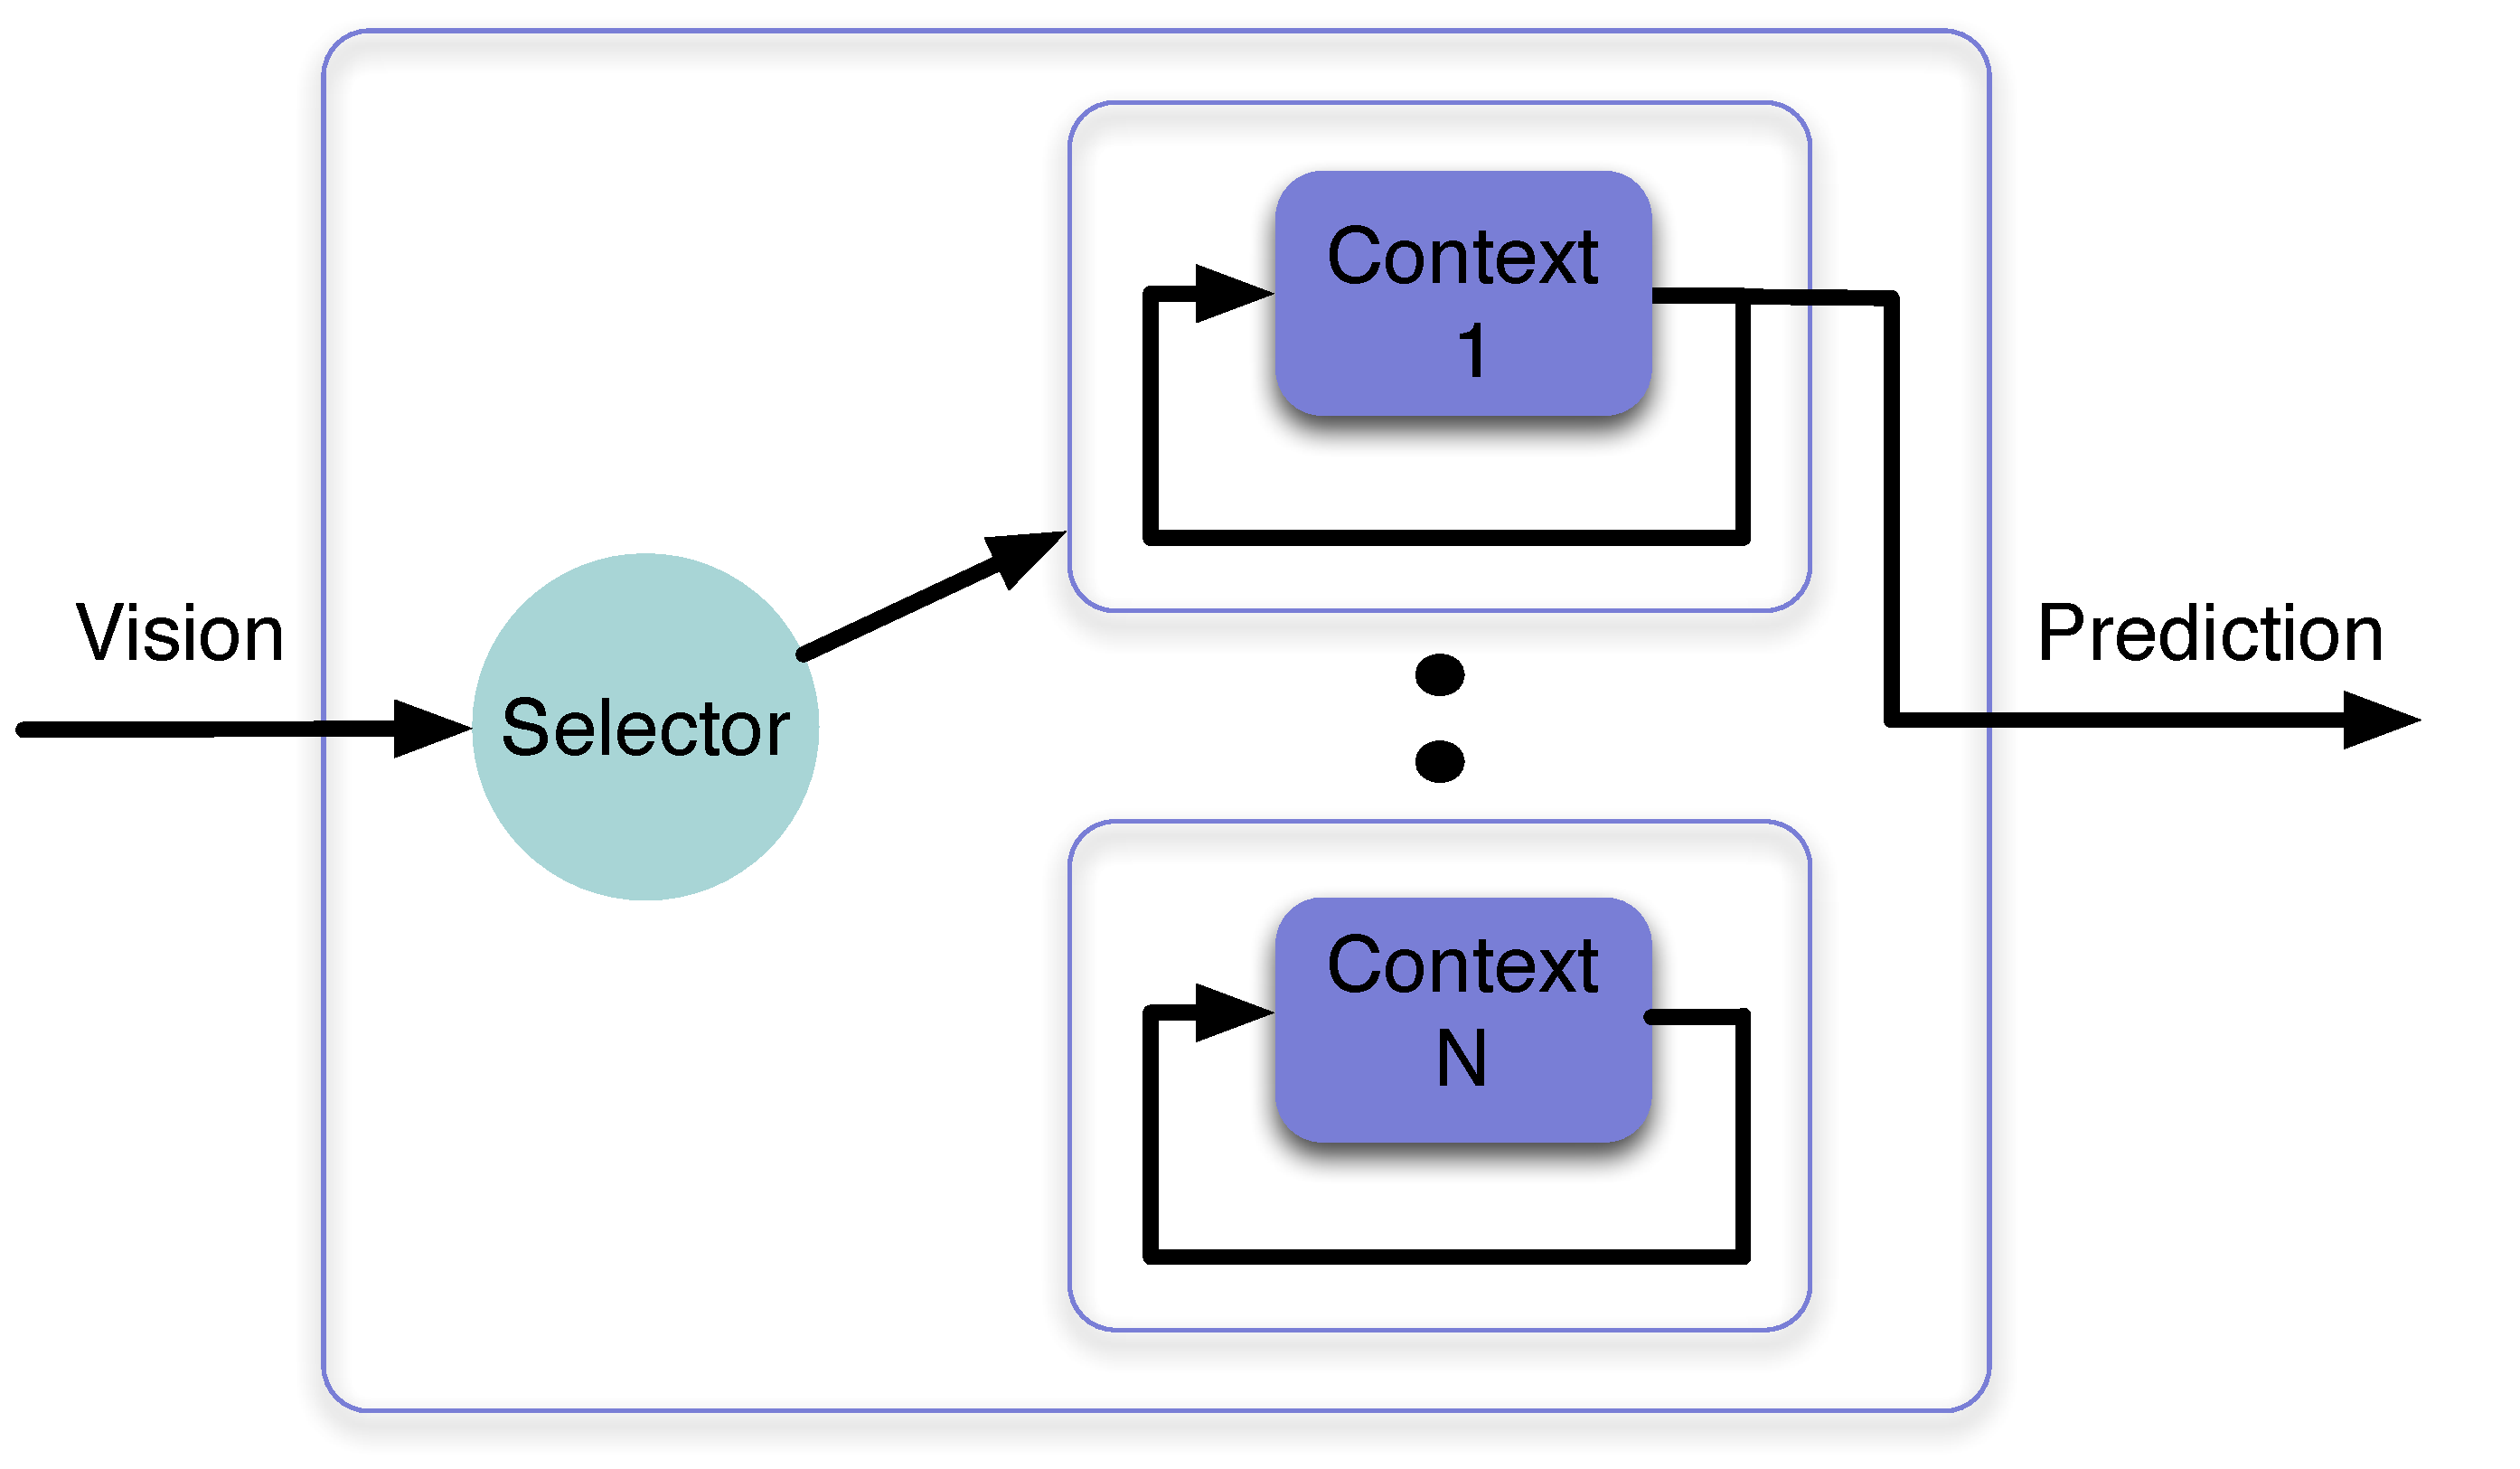
\includegraphics[width=0.9\columnwidth]{modular-schema}}
\caption{A modular prediction scheme for solving problem P1. Visual object identification selects a context/predictor, and gives it the object pose and intended finger trajectory as initial input. Prediction is fed back on itself to produce a multi-step prediction. \label{fig:modular-simple}}
\end{figure}
A different approach is required. Tabula rasa learning is one alternative, but there are problems.  To begin with suppose we try to learn a single predictor from data. The aim would be to predict action effects across a wide range of object shapes and materials. This is hard because the a great deal of variation and complexity must be captured in a single learner. A clue as to a different way to proceed instead comes from computational neuroscience, where models such as MOSAIC employ modular prediction \citep{Haruno_MOSAIC_2008}. Modular means that the overall prediction engine consists of many context specific predictors (Figure~\ref{fig:modular}), where a context is an object, or an object-environment combination. The first advantage of this is that it can be easier to solve many simple learning problems than one complex learning problem. Second, unobservable parameters (frictional coefficients, mass, mass distribution) need not be modelled explicitly but are instead captured implicitly by being associated with a particular context. Whereas MOSAIC couples control and prediction, it avoids real objects (working with simulated mass spring systems). Our work focuses on pure prediction, but for real objects. Our modular prediction scheme uses vision to distinguish the context, by identifying the object shape.

Having explained our overall scheme, we now turn to the mathematical details of how to model robot-object-environment interactions, which will lead in turn to posing the three prediction problems formally.

\begin{figure*}[t!]
\centerline{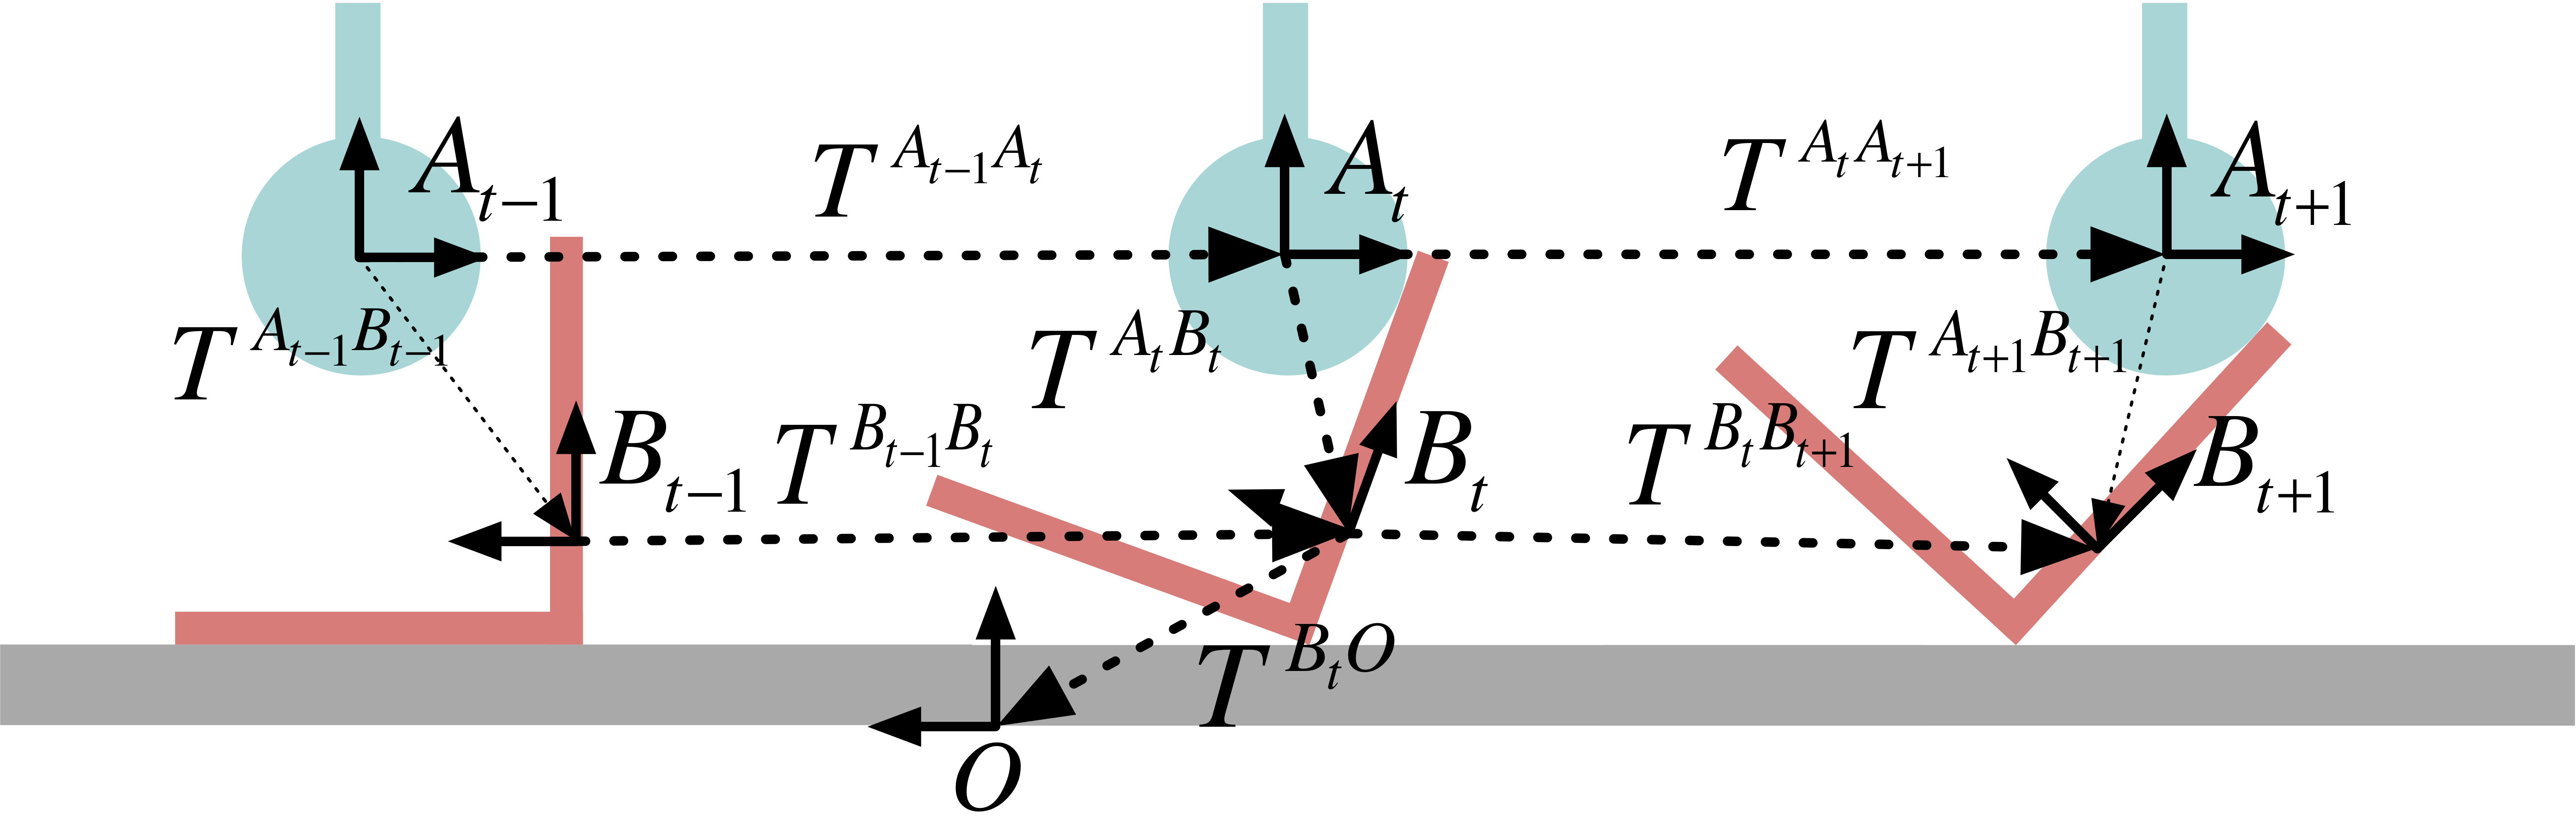
\includegraphics[width=0.8\textwidth]{sequential-frames}
%\includegraphics[width=0.34\textwidth]{similarity}
}
\caption[Setup1]{2D projection at time $t$ of a robotic finger with frame at time $t$ of $A_{t}$,
an object with frame $B_{t}$, and a ground plane with constant frame
$O$. The system can be described using six rigid body transformations %$T^{A_t, B_t}$, $T^{B_t, O}$, $T^{A_{t-1}, A_{t}}$, $T^{A_{t}, A_{t+1}}$, $T^{B_{t-1}, B_{t}}$, and $T^{B_{t}, B_{t+1}}$.
}
\label{fig:Learning.setup1}
\end{figure*}

\section{Encoding rigid body kinematics}
\label{sec:Representations}

In this section we set up the basic notation required to pose the
above prediction learning problems formally. Without loss of generality we explain the notation using an example from our application domain
(Figure~\ref{fig:Learning.setup1}). Three reference frames $A$, $B$
and $O$ sit in a $3$\nobreakdash-\hspace{0pt}dimensional Cartesian
space. Frame $A$ is attached to a robot finger which pushes an object with frame $B$, which in turn is placed on a table top with frame
$O$.\footnote{Although it is an abuse of notation for brevity we will
  use $A$, $B$ and $O$ to denote either the frame or the body to which  it is attached. So we will talk both of the frame $B$ and the object $B$.} While frame $O$ is fixed, $A$ and $B$ change in time and are observed at discrete time steps $..., t-1, t, t+1, ...$.  Frame $X$ at
time step $t$ is denoted $X_t$, and the rigid body transformation
between a frame $X$ and a frame $Y$ is denoted by $T^{X, Y}$.

From classical mechanics we know that in order to predict the change
in state of a rigid body, it is sufficient to know its mass, velocity
and a net force applied to the body.  Since our method will rely on
learning from object trajectories we cannot assume any knowledge of
the mass and applied forces. We can however, use the motion of a body over time to encode acceleration -- an effect of the applied net
force. We therefore use rigid body transformations $T^{X,Y}$ of the interacting bodies through time (Figure~\ref{fig:Learning.setup1}). Given the additional assumption that the net force and the body mass are constant, two subsequent rigid body transformations $T^{B_{t-1},
  B_{t}}$ and $T^{B_{t},B_{t+1}}$ give a complete description of the
state of some body B (here the object) at time step $t$ in the absence
of the other bodies.  Adding the transformation $T^{B_t, O}$ to give a
triple of transformations thus provides a complete description of the
state of body B in the fixed frame $O$ (the stationary elements of the
environment).  Similarly, a second triple of transformations $T^{A_t,
  O}$, $T^{A_{t-1}, A_{t}}$ and $T^{A_{t}, A_{t+1}}$ provides such a
description for some other body (here the finger) with frame $A$. 
The state of the overall system consisting of these two interacting
bodies with frames $A$ and $B$ and the fixed environment $O$ can
thus be adequately described by these six transformations.

In fact in our representation, we replace transformation $T^{A_t, O}$ by relative transformation $T^{A_t, B_t}$, thus also explicitly capturing the spatial relationship and thus any contacts between $A$ (finger) and $B$ (object). This gives us a representation consisting of the set of six transformations marked in bold dotted lines in Figure~\ref{fig:Learning.setup1}. The prediction problem, simply put, will thus be to predict the motion of the object $B$ in the next step: $T^{B_t,B_{t+1}}$ given these five other transformations. Before defining the problem formally, however, we need to think briefly about how best to store these transformations.

Specifically, since we are interested in learning, we need to express this set of transformations in a way that supports generalised predictions. In general the behaviours of interacting bodies described by frames from Figure~\ref{fig:Learning.setup1} are independent of any inertial frame \cite{kopicki_prediction_2010}. Unfortunately, a na\"{\i}ve representation of transformation $T^{A_{t}, A_{t+1}}$ as $A_{t+1}(A_{t})^{-1}$, or explicitly given inertial frame $I$,
% MAREK CHECK
\begin{equation}
T_{in}^{A_{t}, A_{t+1}} = T^{I, A_{t+1}} (T^{I, A_{t}})^{-1}
\label{eq:Learning.In1}
\end{equation}
\noindent makes the transformation in \eqref{eq:Learning.In1} dependent on the currently used inertial frame $I$ (see
Figure~\ref{fig:similarity}).  This would make the stored transformations poor from the point of view of generalisation. A better way is instead to store all the transformations in a body frame (at learning time) and convert to and from an inertial frame dependent transformation (at prediction time) using similarity transforms.

\begin{figure}[b]
\centerline{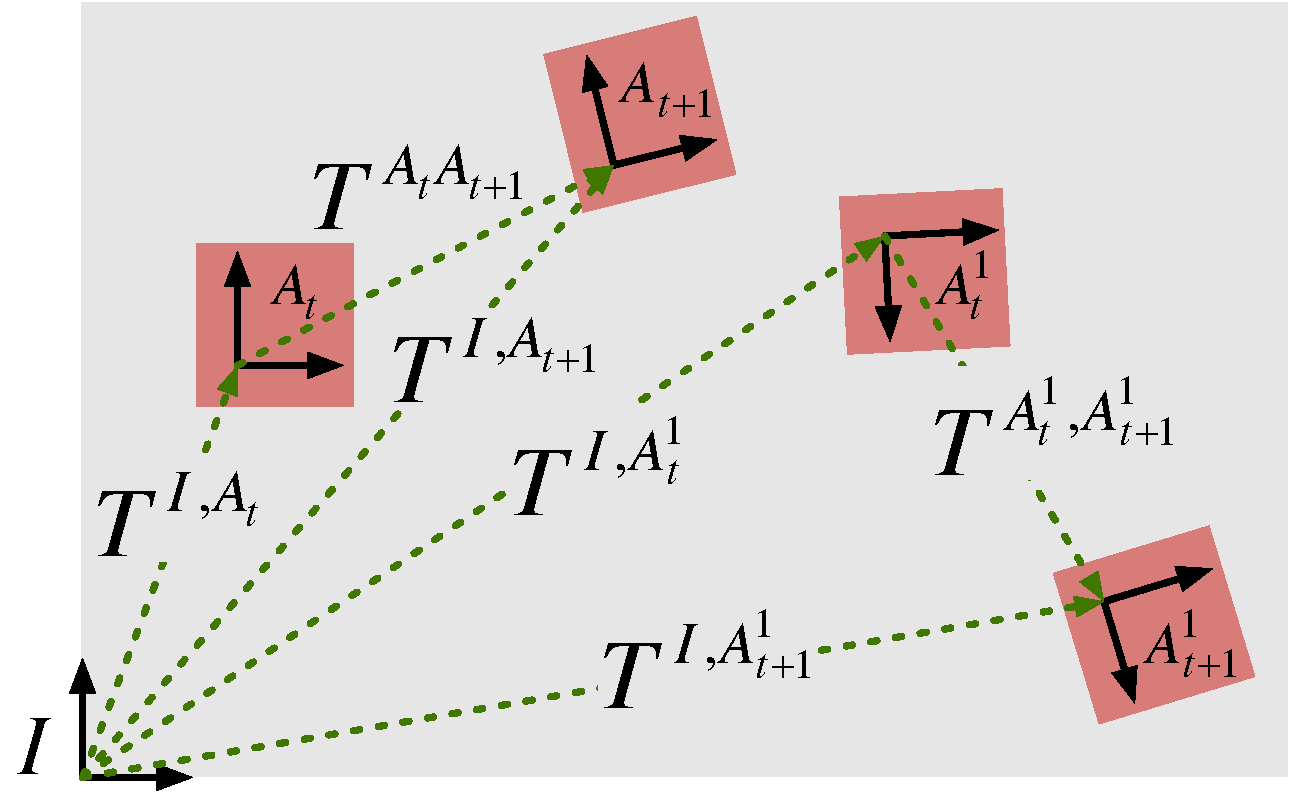
\includegraphics[width=\columnwidth]{similarity-new}}
\caption[Similarity]{ Overhead view of an object on a table starting in two different positions. In each case the motion from $t$ to $t+1$ is the same relative to the instantaneous object body frames $A$ and $A^{1}$. However because transformations $T^{I, A}$ and $T^{I, A^{1}}$ are different, the corresponding transformations in the inertial frame are also different, i.e.\ $T_{in}^{A_{t}, A_{t+1}} \neq T_{in}^{A^{1}_{t}, A^{1}_{t+1}}$.}
\label{fig:similarity}
\end{figure}
Intuitively these similarity transforms align the inertial and body frames, perform the required transformation and then invert the transformation required to align them. In this manner, given the instantaneous object frame $A_{t}$ at time $t$, and the inertial frame dependent transformation
$T_{in}^{A_{t}, A_{t+1}}$, one can obtain the body frame dependent
transformation $T_{body}^{A_{t}, A_{t+1}}$:
\begin{equation}
T_{body}^{A_{t}, A_{t+1}} = (T^{I, A_{t}})^{-1} T_{in}^{A_{t}, A_{t+1}} T^{I, A_{t}}
\label{eq:Learning.Body1}
\end{equation}
\noindent where $T^{I, A_{t+1}} =$ $T_{in}^{A_{t}, A_{t+1}} T^{I, A_{t}} =$ $T^{I, A_{t}} T_{body}^{A_{t}, A_{t+1}}$.

It is this body frame dependent transformation that will be stored during learning. Conversely, when a prediction is required, given a body frame dependent transformation, the object
frame $A_{t}$, and using Equation~\eqref{eq:Learning.Body1}, the
inertial frame dependent transformation $T_{in}^{A_{t}, A_{t+1}}$ is
recovered using:
\begin{equation}
T_{in}^{A_{t}, A_{t+1}} = T^{I, A_{t}} T_{body}^{A_{t}, A_{t+1}} (T^{I, A_{t}})^{-1}
\label{eq:Learning.Body2}
\end{equation}
This technique is critical to generalisation across inertial frames. In the rest of the paper we will retain subscripts $in$, but suppress subscripts $body$, and assume that all transformations $T^{X, Y}$ are transformations in the body frame $X$ related to the equivalent transform in some inertial frame using a similarity transform:
\begin{equation}
T^{X, Y} \equiv T_{body}^{X, Y} = ({T^{I, X}})^{-1} T_{in}^{X, Y} {T^{I, X}}
\label{eq:Learning.Similarity}
\end{equation}

\section{Formal statement: learning to predict}
\label{sec:PredictionProblem}

We now have the basics required to formally describe the one-step and then the multi-step prediction
problem in such a way that they become problems of learning to predict, and we can effectively tackle Problem 1 (Action Interpolation).

\subsection{One step prediction.} The one step prediction problem is formulated as follows: given that we observe the recent and current positions of the finger and object, and know the planned motion of the finger, $T^{A_{t},  A_{t+1}}$, predict the resulting immediate motion of the object,
$T^{B_{t}, B_{t+1}}$.  This is a problem of finding a function~$f$:
\begin{multline}
f:T^{A_t, B_t}, T^{B_t, O}, T^{A_{t-1}, A_{t}}, T^{B_{t-1}, B_{t}}, T^{A_{t}, A_{t+1}} \\ \longrightarrow T^{B_{t}, B_{t+1}}
\label{eq:Learning.long}
\end{multline}

The function $f$ is capable of describing the effects of interactions between rigid bodies $A$ and $B$, providing their physical properties and net forces are constant
in time,\footnote{A dynamic formulation could explicitly incorporate
net forces into the domain and codomain of \eqref{eq:Learning.long}.}
in the limit of infinitesimally small time steps.
Furthermore, it can be approximately learned from observations
for some small fixed time interval $\Delta t$ between time steps.

If robotic manipulations are performed slowly we can assume quasi-static conditions, and ignore all frames at time $t-1$.  This conveniently reduces the dimensionality of the problem, giving a simplified function~$f_{qs}$:
\begin{multline}
f_{qs}: T^{A_t, B_t}, T^{B_t, O}, T^{A_{t}, A_{t+1}} \longrightarrow T^{B_{t}, B_{t+1}}
\label{eq:Learning.short}
\end{multline}

\subsection{Multi-step prediction.} Having stated the one-step prediction problem it is possible to solve
the multi-step prediction problem. Given a predictor (either $f$ or
$f_{qs}$), the initial state of the finger $T^{A_{1}, O}$ and object
$T^{B_{1}, O}$, and knowing the trajectory of the finger $A_{1},
\ldots A_{T}$ over $T$ time steps, one can predict the complete
trajectory of the object $B_{1}, \ldots B_{T}$, by simply iterating
the predictions obtained from $f_{qs}$.  That is, the output of the
predictor at time~$t$ is used as the input to the predictor for the
next time step (Figure~\ref{fig:modular-simple}). While this is a well known approach, it is a hard problem to produce a predictor that will behave well over many time steps. Over time all predictors will diverge from reality. Thus an empirical question is whether for a particular domain and prediction scheme, predictions are reasonably close to reality for a suitable number of steps. It is precisely a multi-step prediction problem that is solved in this paper with the algorithms described below.

\subsection{Learning to predict as regression.} In principle it is straightforward to acquire a predictor $f$ or
$f_{qs}$ by learning it from data. Given sufficient experience of
object and finger trajectories we can perform a nonparametric
regression analysis by taking $T^{A_t, B_t}$, $T^{B_t, O}, T^{A_{t},
  A_{t+1}}$ as independent variables, and $T^{B_{t}, B_{t+1}}$
as the dependent variable.  Nonetheless a powerful regression
technique is needed since the domain of $f_{qs}$ has 18~dimensions
or more depending on the parameterisation of motion.

\subsection{Learning to predict as density estimation.} As an alternative to learning the mapping~\eqref{eq:Learning.short} by regression, we can recast $f_{qs}$ as a conditional probability density (CPD) $p_{qs}$ over possible object motions $T^{B_{t},B_{t+1}}$ \citep{kopicki_prediction_2009}:
\begin{equation}
p_{qs}(T^{B_{t}, B_{t+1}} | T^{A_t, B_t}, T^{B_t, O}, T^{A_{t}, A_{t+1}})
\label{eq:Learning.density1}
\end{equation}

The learning problem is then posed as one of density estimation, permitting the modelling of the probabilities of many possible outcomes. 

Either the regression or density estimation formulation can be used in a modular scheme. In that case a separate module is learned for each combination of agent, object, and environment . Each module interpolates over actions for its context, and thus the system solves problem P1: Action Interpolation for multiple contexts. There is not, however, enough information in the five transformations used as input, to solve either problem P2 (Action Transfer) or problem P3 (Shape Transfer). We now identify the additional information needed to solve these.

\section{Transfer Learning: Representing contacts}
\label{sec:InfoForPrediction}
\begin{figure}[t]
\centerline{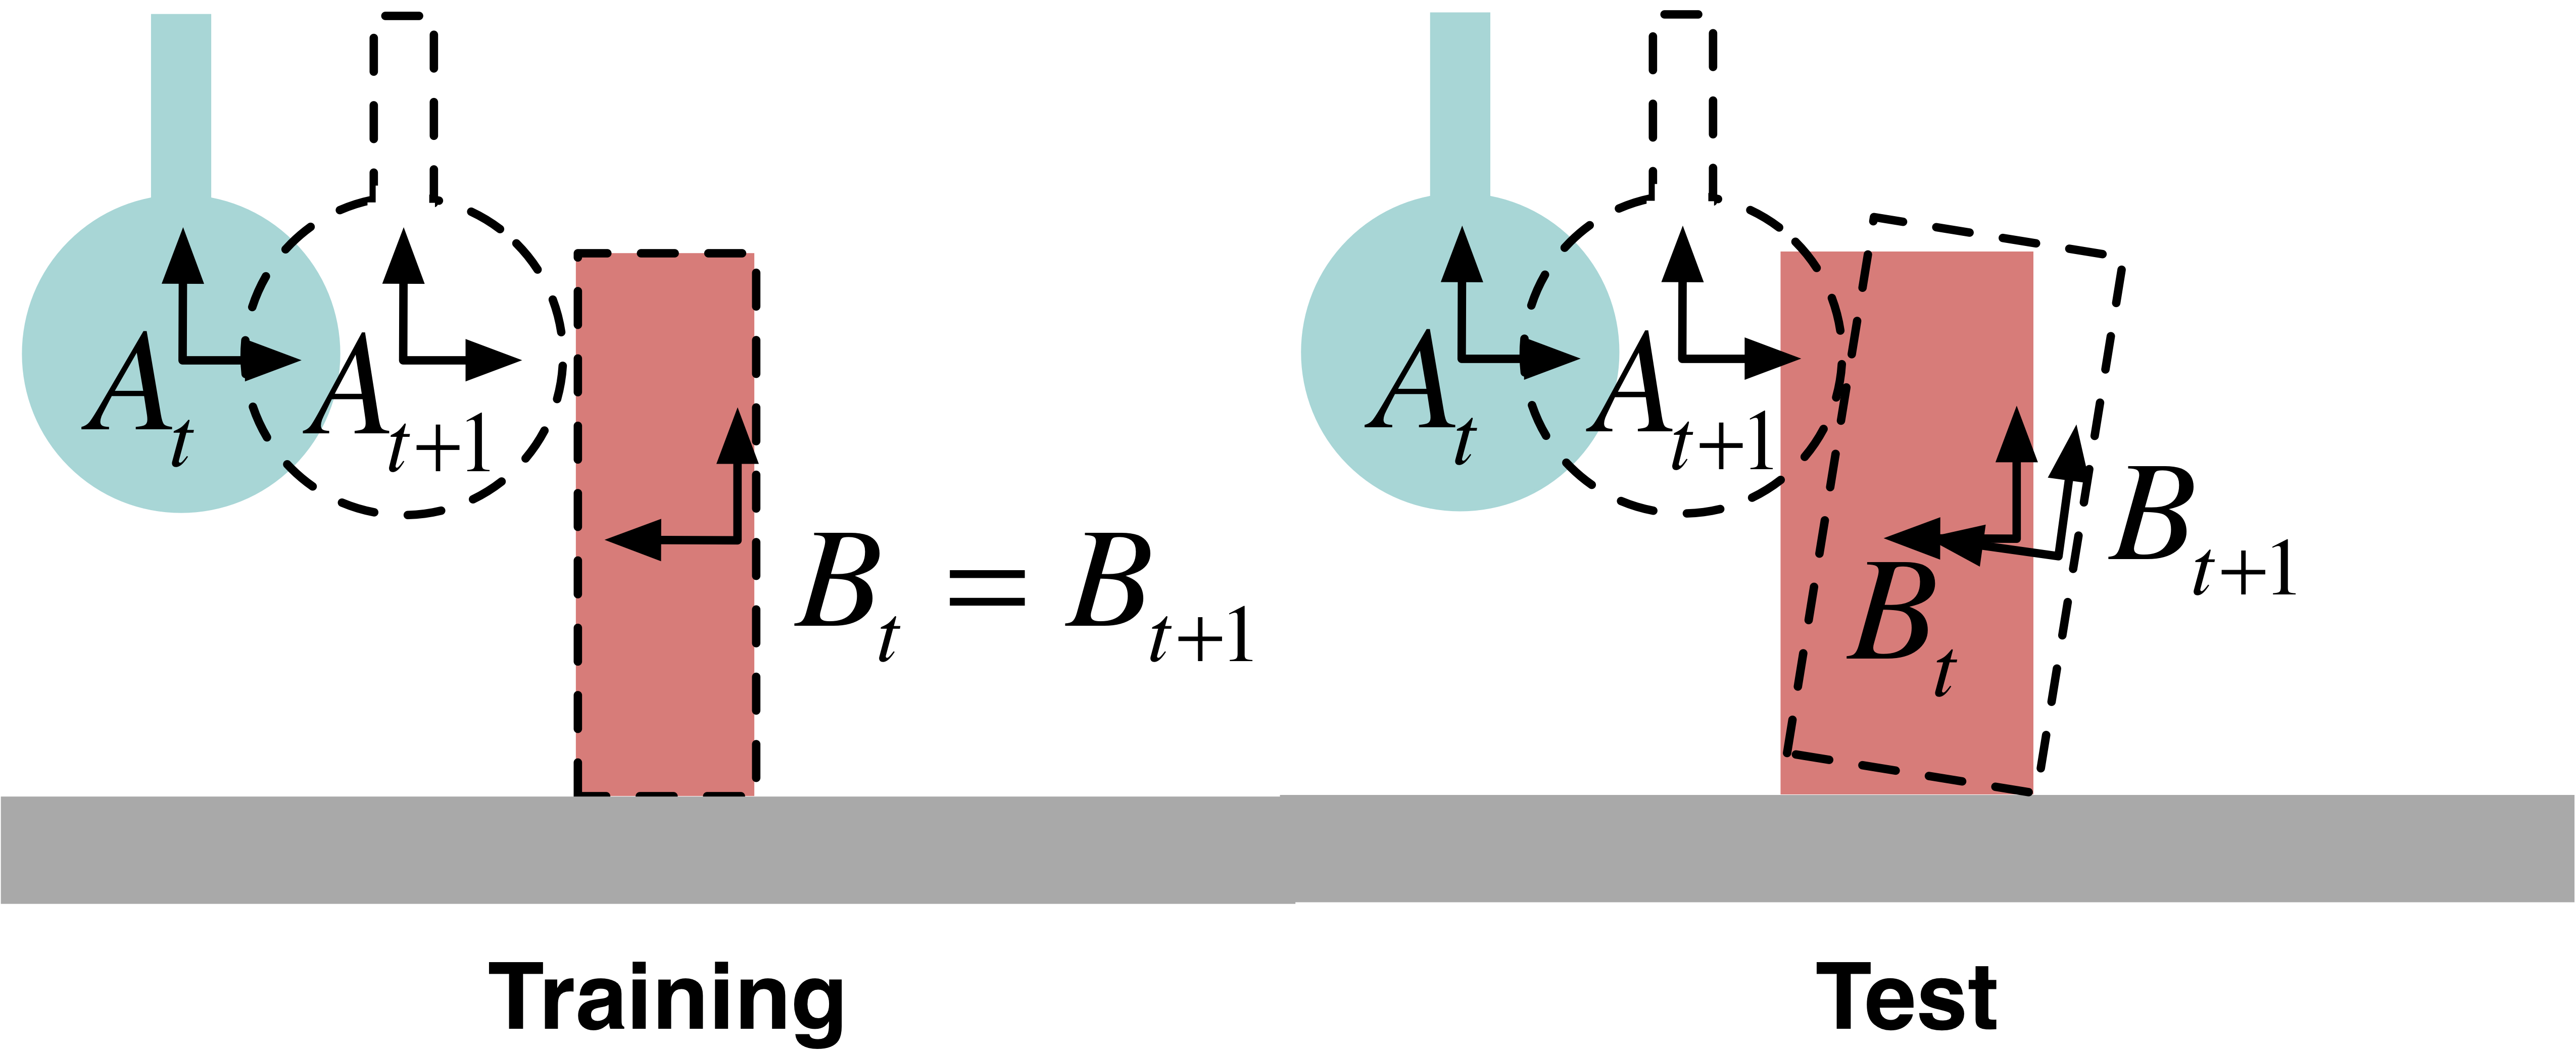
\includegraphics[width=\columnwidth]{shapes-colour}}
\caption[Shapes]{Two scenes (left and right),
each with an object on a tabletop. Only the shape of object $B$ differs between the scenes. Yet when finger A moves as shown by the dashed outline at time $t+1$, the resulting transformation of $B$ will be quite different.}
\label{fig:Learning.shapes}
\end{figure}
The input domains of $f$, $f_{qs}$, and $p_{qs}$ are insufficient to pose problems P2 (Action Transfer) or P3 (Shape Transfer). This is because they only capture the {\em global} relations between objects. To properly pose transfer learning the input domain must capture all the {\em local} contact relations between the object and its surroundings.  To see why, consider Figure~\ref{fig:Learning.shapes}. On the left is a training example. On the right is a test case, where the object is wider. Given the same placement of the frames on object and agent, and the same finger motion, the predicted behaviour using Equation~\eqref{eq:Learning.short} will be the same as for the training example. This is wrong. For the correct prediction to be transferred, additional information is needed on the contact between $A$ and $B$. This can be captured by attaching additional frames to $A$ and $B$ close to their point of contact (see Figure~\ref{fig:Learning.setup2}, centre panel).
\begin{figure*}[t]
\centerline{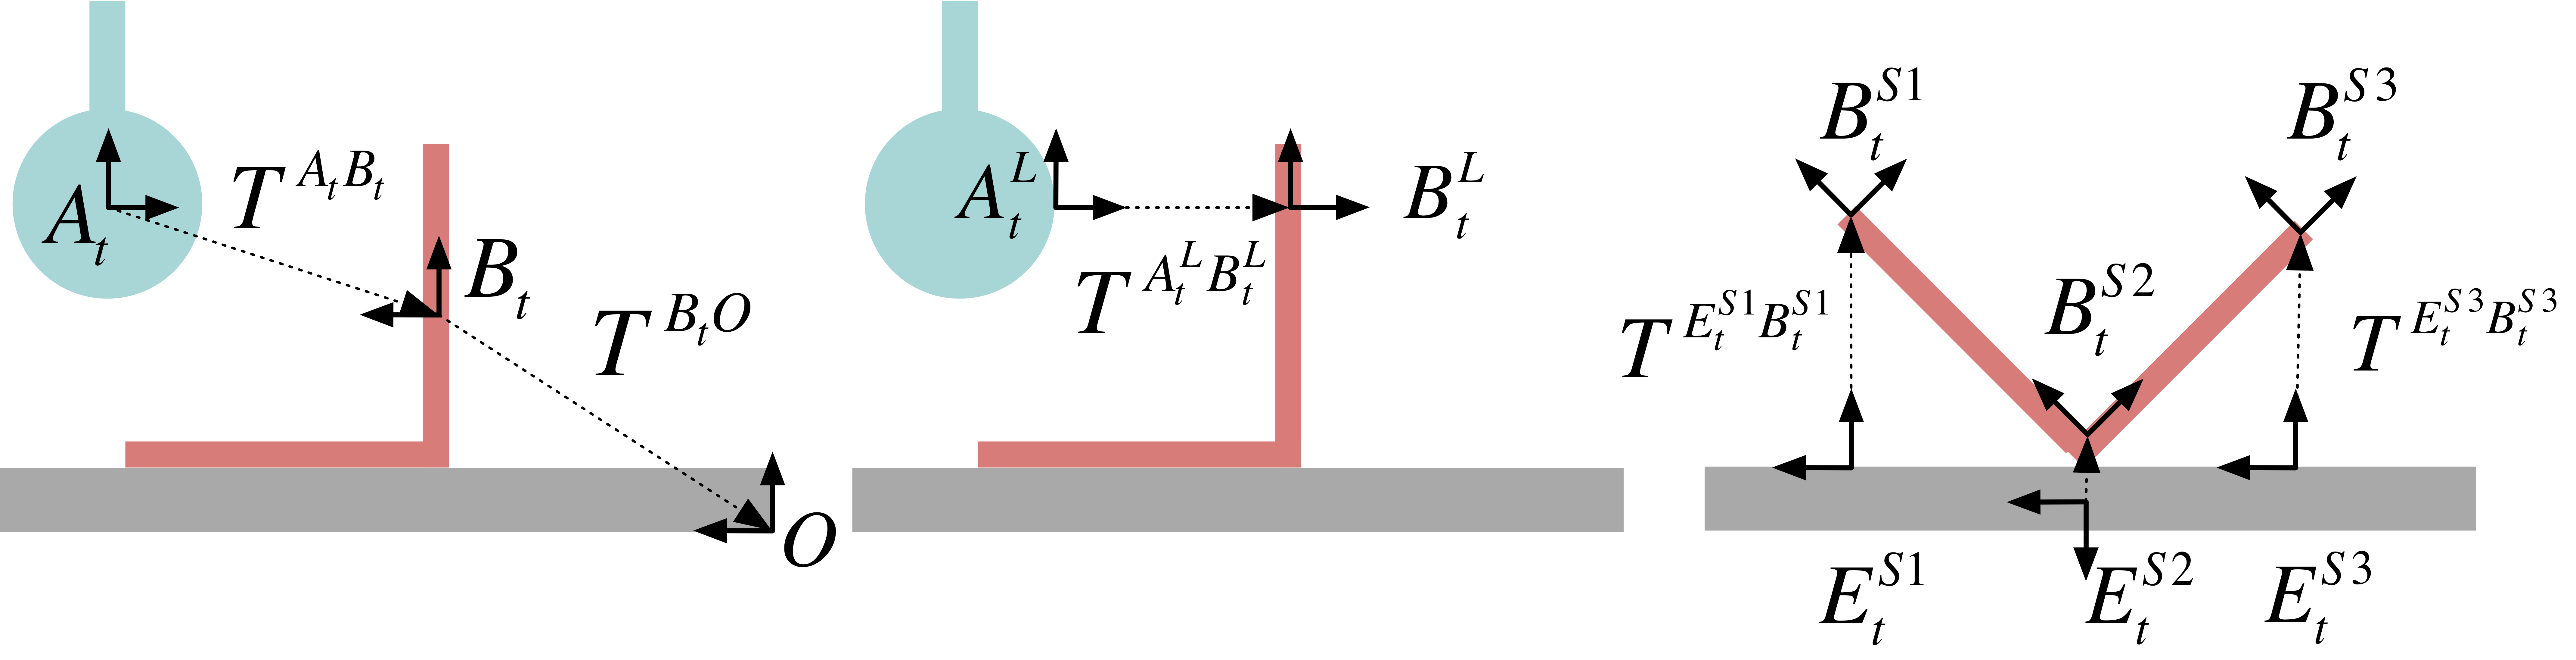
\includegraphics[width=\textwidth]{information}}
\caption{Three types of information useful in prediction problems. Left: (G - global) global frames of reference for the robot, object and the world. Centre: (A - agent) local frames of reference on the robot finger and the closest point on the object. Right (E - environment) local frames of reference on the object and the closest points on surfaces in the environment.}
\label{fig:Learning.setup2}
\end{figure*}
In general, an object has multiple contacts with the robot and the environment. Each of these contacts provides a kinematic constraint on the object's motion, and thus each one should be modelled. Rigid body simulators use just such contact information. 

We use a pair of local frames to encode each contact or near contact. Each pair encodes one transformation between part of the object $B$ and another body.  To distinguish these local frame pairs from what has gone before we henceforth refer to the main frame attached to a body (defined in Section~\ref{sec:Representations}) as that body's global frame. We define the local frame pairs as follows. Consider Figure~\ref{fig:Learning.setup2}  (left panel). We first define a pair of local frames capturing the finger-object contact as $A^{L}_{t}$ and $B^{L}_{t}$ (centre panel). These are spatially dynamic, i.e.\ at any time $t$ they are located at the points of closest proximity on the finger and object respectively.  We define the \textit{agent-object contact}
information as the transformations $T^{A^{L}_{t}, A^{L}_{t+1}}$ and $T^{A^{L}_t, B^{L}_t}$.

We also define local frame pairs to model object-environment contacts. One frame is attached to some point on the object ($B^{Sk}_t$), and one is attached to the nearest point in the environment $E^{Sk}_t$.  Thus the environment frame within each pair is spatially dynamic, changing its position as the object moves. If $N$ points on the object are chosen for modelling there will be $N$ pairs of local frames $B^{Sk}_t$ and $E^{Sk}_t$ to capture the object-environment contacts at time $t$, where ($k=1 \ldots N$) (Figure~\ref{fig:Learning.setup2} right panel). Using these frame pairs we then define the \textit{object-environment contact} information as the set of transformations $T^{E^{Sk}_t,B^{Sk}_t}$ for $k=1 \ldots N$. 

During training a single type of contact model is learned by pooling data from frames located at several points on the object. During transfer this single model is copied, creating several identical contact experts on the new object. An extension would be to condition a number of such contact models by the local shapes at the contacts, and this is an intended line of future work. We hypothesize that both data pooling and conditioning will be important elements in improving the transfer of predictions. Additionally, to obtain the results presented in this paper, the number and the locations of the frames $B^{Sk}_t$ on each different object were determined empirically.\footnote{This procedure could be automated.} Finally, we note that we have motivated these contact experts as enabling shape transfer, but they are equally applicable to action transfer. The top row of Figure~\ref{fig:ToyExample} shows a training and a test case for problem P2 (action transfer). The prediction for the test case requires encoding of the kinematic constraint imposed by the contact between the base of the L-shaped flap and the table. This constraint exists in the training push, but was not significant since the flap could rotate on its corner.

We can now consider the effects that different sets of information might have. A predictor possessed only
of global frames for each body we refer to as having global information (G). We add agent-object contact
information (G+A), and object-environment contact information (G+A+E). Now consider the possible predictions for the test case (Figure~\ref{fig:ToyExample} bottom row). A predictor using G will predict that the object will not move. A predictor using G+A has information from the training case that the object surface will move with the finger, so that the finger will not pass through it, but is also capable of predicting that the object rotates about the corner and into the table since it doesn't model the object-environment contact. A predictor using G+A+E will have information about the effect of the contact between the base of the flap and the table and so should avoid predicting a rotation into the table.
\begin{figure}[b]
\centerline{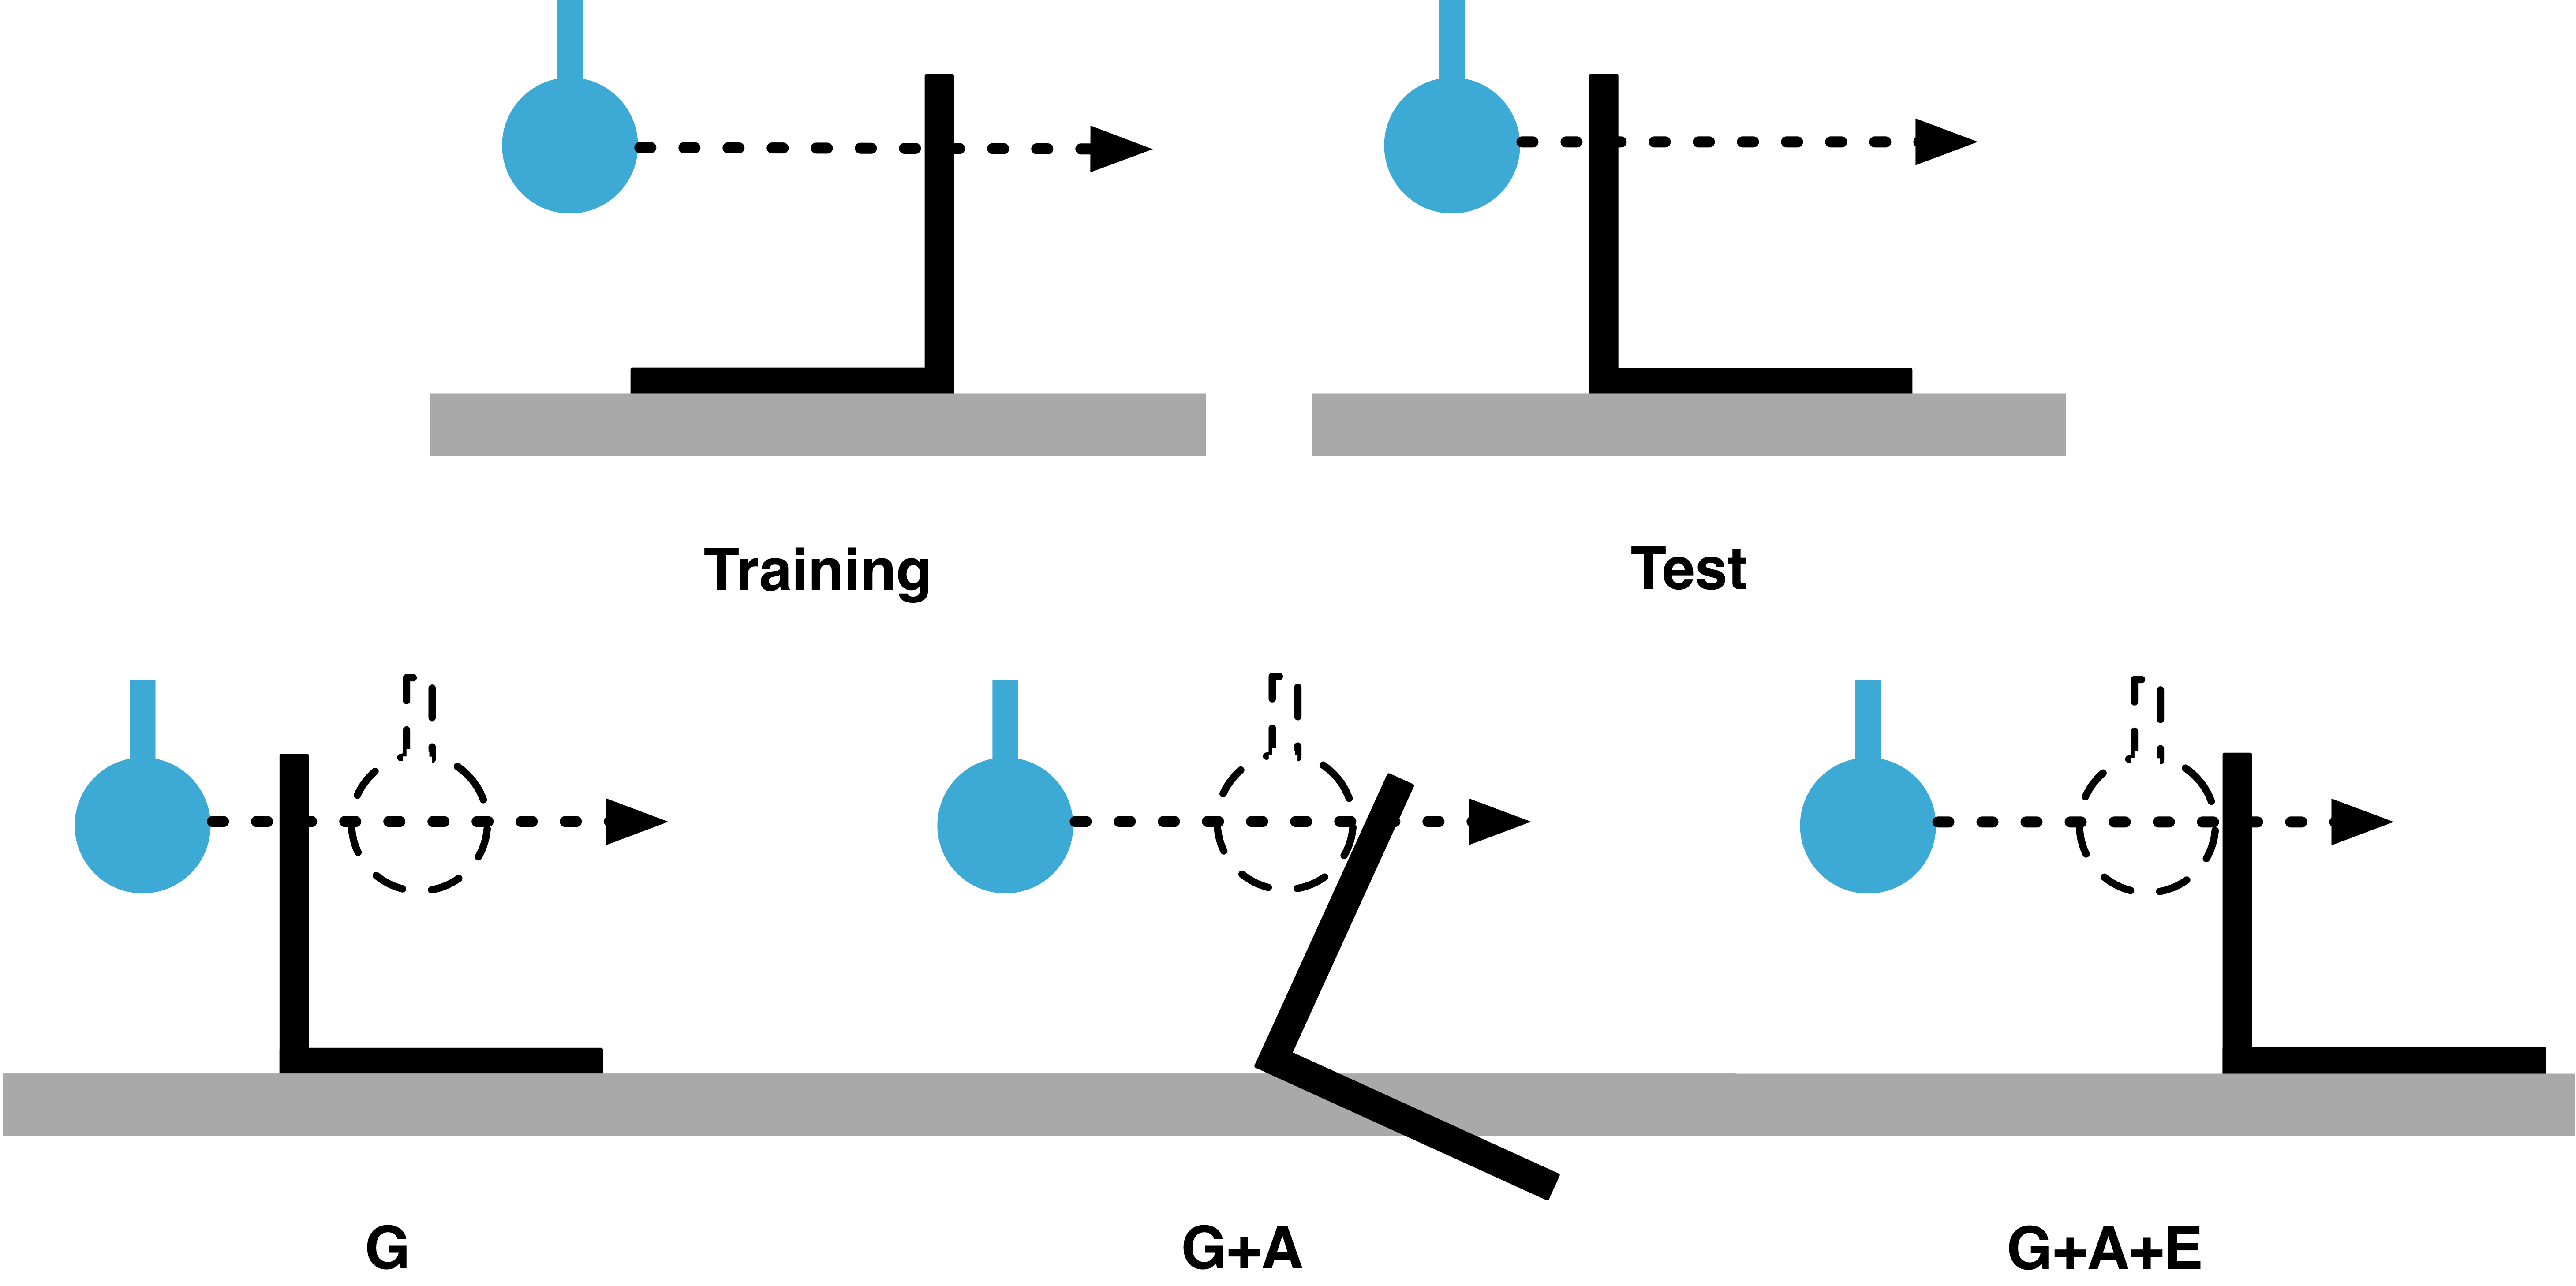
\includegraphics[width=\columnwidth]{BackPushToyExample}}
\caption[ToyExample]{Information for Action Transfer: an L-shaped object is pushed by a finger. Various predictors are trained solely on forward pushes (top left), but tested on backwards pushes (top right). The top panels show a training and a test push, whereas the bottom panels show predictions given different information (G, G+A and G+A+E) for the test push.}
\label{fig:ToyExample}
\end{figure}
One point is critical here: the above analysis only concerns what the information allows, it depends on the ability of the learner to
utilise it.  To test this we must incorporate the information into each learning framework. We can simply extend the regression and density
estimation frameworks to achieve this. For regression one way to incorporate the extra information $A^{L}_{t}$,$B^{L}_{t}$ and
$E^{Sk}_t$\hspace{-6pt}, $B^{Sk}_t$, provided by the agent and environment contacts, is simply to enlarge the domain of function~$f$
in Equation~\eqref{eq:Learning.short}, that is:
\begin{multline}
f'_{qs}: T^{A_t, B_t}, T^{B_t, O}, T^{A_{t}, A_{t+1}}, T^{A^{L}_t, B^{L}_t} \\ \{, T^{E^{Sk}_t,B^{Sk}_t}\}_{k=1 \ldots N} \longrightarrow T^{B_{t}, B_{t+1}}
\label{eq:Learning.augmented}
\end{multline}
\noindent Unfortunately, because the dimensionality of the domain of $f'_{qs}$ grows with the number of environment contacts $N$,
the difficulty of learning the mapping $f'_{qs}$ rapidly increases as environment contacts are added.

The conditional probability density (CPD) $p_{qs}$ over possible object motions $T^{B_{t}, B_{t+1}}$~\citep{kopicki_prediction_2009} is augmented as follows:
\begin{multline}
p_{qs}(T^{B_{t}, B_{t+1}} | T^{A_t, B_t}, T^{B_t, O}, T^{A_{t}, A_{t+1}}, T^{A^{L}_t, B^{L}_t} \\ \{, T^{E^{Sk}_t,B^{Sk}_t}\}_{k=1 \ldots N})
\label{eq:Learning.density}
\end{multline}

Again the dimensionality of the conditioning variables makes density estimation hard as the number of contacts grows. One way around this in the density estimation case is to factorize the density in a way that reflects the contact structure. We consider this in the next section. 

\section{Factorised density estimation}
\label{sec:Factors}

Both formulations give learning problems that increase in difficulty as further contacts are added. One question is whether either formulation can be recast so as to take advantage of the natural
problem structure. This section presents one such scheme for the
density estimation (or CPD) formulation, based on a product of experts.

Specifically the CPD formulation allows us to factorise the density
and approximate $p_{qs}$ by making a conditional independence
assumption. The unfactored CPD formulation gives a density over
possible one step motions of the object. We can
factorise this by breaking up the conditioning variables into groups
according to the contacts. This reflects the notion that the behaviour
at one contact is independent of the other contacts: each component of the
product is an expert encoding the likely object motions given a single
kinematic constraint. The product will be maximised by a
motion that best satisfies all the constraints simultaneously.

The computational advantage is that since the component
densities factorise the conditioning variables of $p_{qs}$ their
domains' dimensionalities are smaller, and so potentially they can
better manage the complexity of incorporating more information into
the predictor.  Furthermore, the subset of experts used in the product can be selected dynamically, depending for example on the current set of contacts. Schematically, for some normalisation constant~$C$ we propose the following factorisation:
\begin{equation}
p_{qs} \approx C\ p_{global}\ p_{agent}\ \mathop{\prod}_{k=1 \ldots N}{ p_{env,k}}
\label{eq:Learning.product}
\end{equation}
\noindent where
\begin{subequations}
\begin{align}
p_{global} &\equiv p_{global}(T^{B_{t}, B_{t+1}}|T^{A_{t}, A_{t+1}}, T^{A_t, B_t}, T^{B_t, O})
\label{eq:Learning.densityglobal} \\
p_{agent} &\equiv p_{agent}(T^{B^{L}_{t}, B^{L}_{t+1}}|T^{A^{L}_{t}, A^{L}_{t+1}}, T^{A^{L}_t, B^{L}_t})
\label{eq:Learning.densitylocal} \\
p_{env,k} &\equiv p_{env,k}(T^{B^{Sk}_t, B^{Sk}_{t+1}} | T^{E^{Sk}_t,B^{Sk}_t})
\label{eq:Learning.densityenv}
\end{align}
\end{subequations}

\noindent denote the \textit{global}, \textit{agent-object} and
$k^{th}$ \textit{object-environment} density factors
respectively~\cite{kopicki_prediction_2009}\cite{kopicki_prediction_2010}. 
The one step prediction problem can then be defined as finding the
transformation $\widetilde{T}_{in}^{B_{t}, B_{t+1}}$ expressed in some inertial frame which maximises the product of densities \eqref{eq:Learning.product}:
\begin{equation}
\widetilde{T}_{in}^{B_{t}, B_{t+1}} = \argmax{T_{in}^{B_{t}, B_{t+1}}} \bigg\lbrace
p_{global}\  p_{agent} \mathop{\prod}_{k=1 \ldots N}{ p_{env,k} }
\bigg\rbrace
\label{eq:Learning.MultiFactorProduct}
\end{equation}

\noindent where similarity transforms as described in Section~\ref{sec:Representations} must be used to evaluate $p_{global}$, $p_{agent}$ and the $N$ environment factors $p_{env,k}$ for a given ${T}_{in}^{B_{t}, B_{t+1}}$.
\begin{figure}[t]
\centerline{\includegraphics[width=\columnwidth]{product-predictor}}
\caption[Factored Prediction]{ A Dynamic Product of Experts. This gives the structure of a factorised predictor for a single context as depicted in the modular learner in Figure~\ref{fig:three-prediction-problems}. Each expert in the product has an applicability condition which determines whether it contributes to the product. The applicable predictors combine densities over predictions to produce an overall density. This is optimised to produce a specific prediction.}
\label{fig:modular}
\end{figure}

The key property here is that the global, agent and environment densities encode different information about which rigid body transformations are feasible. By taking the product of these densities, only transformations which are feasible in all factors' frames will have high probability in the resulting combined distribution. In addition we make this product dynamic in the number of object-environment factors. Once the object surface is beyond some threshold distance from the environment surface its predictor switches off, and when it is close enough it switches on again. This enables us to keep only relevant predictors in the product at any one time -- improving prediction quality and efficiency. 

In summary we have now described two main formulations (regression and density estimation) able to incorporate varying amounts of information (G, G+A, G+A+E). We have also presented a reformulation of density estimation that factorises the prediction problem given information G+A or G+A+E into a product of experts. Which which information and problem formulation combine to provide the best prediction framework?
Is the factorised problem better able to exploit the additional
information than the unfactorised version? These questions can only be
answered using specific regression and density estimation
algorithms. Having completed our problem formulation we therefore now
turn to the details of the implementations we used for each framework.

\section{Implementation}\label{sec:Implementation}

\newcommand{\bx}{\mathbf{x}}
\newcommand{\by}{\mathbf{y}}

The implementations are indexed by the algorithms used, and the information employed. For the function approximation formulation we used Linear Weighted Projection Regression (LWPR). For the unfactored density estimation formulation we used a variant of Kernel Density Estimation (KDE), and for the factored density estimation formulation we also used KDE, but denote it KDEF where -F denotes the use of factorisation. In addition, each algorithm: LWPR, KDE, KDEF, was implemented with differing amounts of input information. We denote these G (Global), GA (Global and Agent) and GAE (Global and Agent and Environment), as described previously. All the implementations depend on the parameterisation of rigid-body transformations chosen. In this paper we tested two parameterisations of orientation: Euler angles and quaternions (see e.g. \citep{murray_mathematical_1994}). We also employed two different densities for the quaternion parameterisation: Gaussian and von-Mises Fisher.

%%%%%%%%%%%%%%%%%%%%%%%%%%%%%%%%%%%%%%%%%%%%%%%%%%%%%%%%%%%%%%%%%%%%%%%%
\subsection{Regression method}\label{sec:Implementation.regression}

Locally Weighted Projection Regression (LWPR) \citep{vijayakumar_incremental_2005} is a powerful method applied widely in robotics, to estimate the mapping described by Equation~\eqref{eq:Learning.short}. The regression scheme was implemented using the LWPR software library \citep{klanke_library_2008}. LWPR was chosen because it employs an incremental learning algorithm that can handle a large number of input dimensions. After initial experimentation LWPR was run using the Euler angle parameterisation. The dimensions of the input and output spaces of each LWPR predictor are summarised in Table~\ref{tab:InpOutSpace}.

%\begin{table}[b]
%\begin{center}
%\begin{tabular}{|l|l|l|}
%\cline{1-3}
%Predictor & input space & output space \\
%\cline{1-3}
%LWPR-G euler & 18 & 6 \\
%LWPR-GA euler & 24 & 6 \\
%LWPR-GAE euler & 24 + N*6 & 6 \\
%\cline{1-3}
%\end{tabular}
%\end{center}
%\caption[Input/output space LWPR]{Dimensions of input and output spaces
%of LWPR predictors, where $N$ is the number of
%"environment contacts".}\label{tab:InpOutSpaceLWPR}
%\end{table}


%%%%%%%%%%%%%%%%%%%%%%%%%%%%%%%%%%%%%%%%%%%%%%%%%%%%%%%%%%%%%%%%%%%%%%%%
\subsection{Kernel density method}\label{sec:Implementation.kde}

A variant of Kernel Density Estimation (KDE) \citep{scott2004multi-dimensional} is used to approximate the conditional densities employed in the product in Equation~\eqref{eq:Learning.MultiFactorProduct}. This requires that we encode the rigid body transformations as parameter vectors. To that end, and for the sake of compactness, we introduce some additional notation. First $T^{\bx_f}$ is used to denote the set of conditioning transformations for factor $f \in \{G, A, (E,1) \ldots (E,N)\}$, and $T^{\by_f}$ for the corresponding conditioned transformation. $\bx_f$ and $\by_f$ are then simply the corresponding parameter vectors for a given parameterisation. Given this the global factor, for example, can be referred to in three equivalent ways:

\begin{eqnarray}
p_G(T^{B_{t}, B_{t+1}}|T^{A_{t}, A_{t+1}}, T^{A_t, B_t}, T^{B_t, O}) \\ \equiv p_G(T^{\by_G}|T^{\bx_G})  \\
\equiv p_G(\by_G|\bx_G)
\end{eqnarray}

Finally we define the parameter vectors for the unfactored density estimation problem Eq.\eqref{eq:Learning.density} as the concatenation of the vectors for each factor, so that

\begin{equation}
\bx= \langle \bx_G, \bx_A, \{\bx_{E,k}\}_{k = 1 \ldots N} \rangle
\end{equation}

\begin{equation}
\by = \langle \by_G, \by_A, \{\by_{E,k}\}_{k = 1 \ldots N} \rangle
\end{equation}

So as to capture the conditional probability densities (CPD) over $\by_f$ for all the different values of $\bx_f$ we simply perform kernel density estimation for their joint density, and then  index by the specific $\bx^t$ at prediction time to give $p_f(\by_f^t|\bx_f^t)$. For factor $f$ the joint density kernel estimate is:
\begin{equation}
p_f(\by_f,\bx_f) \propto \mathop{\sum}_{j=1 \ldots M}
K_{\mathbf{H}^{\bx_f}}(\bx_f - \hat{\bx}_f^j)
K_{\mathbf{H}^{\by_f}}(\by_f - \hat{\by}_f^j)
\label{eq:Density.Estimation.mixture}
\end{equation}
\noindent where the bandwidth matrices  $\mathbf{H}^{\bx_f} $ and $\mathbf{H}^{\by_f} $ are diagonal, so that $\mathbf{H}^{\bx_f}_{ii}  = \theta \mathbf{h}^{\bx_f}_i$. Vectors $\mathbf{h}^{\bx_f}$ and $\mathbf{h}^{\by_f}$  are estimated from training samples using Silverman's ``multivariate rule-of-thumb'' \citep{scott2004multi-dimensional}. The additional scaling parameter $\theta \in \mathbb{R}$ is estimated by model selection (see Subsection~\ref{sec:Experiment.Setup}). Note that $\mathbf{H}^{\bx_f}$ and $\mathbf{H}^{\by_f}$ depend on the factor $f$ being estimated. Given that they are diagonal, and suppressing $f$ and $\theta$ for compactness, each kernel function $K()$ in Equation~\eqref{eq:Density.Estimation.mixture} can thus be written:
\begin{equation}
K_{\mathbf{H}^\bx}(\bx - \hat{\bx}) = \exp \left[-\frac{1}{2}d(\bx, \hat{\bx}, \mathbf{h^{x}}) \right]
\label{eq:Density.Estimation.kernel}
\end{equation}

%\begin{equation}
%K(\bx, \hat{\bx}, \mathbf{h}) =
%\mathop{\prod}_{l=1 \ldots L} \exp \left[-\frac{1}{2}d(\bx_l, \hat{\bx}_l, \mathbf{h}_l)\right]
%\label{eq:Density.Estimation.kernel}
%\end{equation}
%\noindent where the $\bx_l$ are the parameters of the $L$ transformations that are the conditioning variables in the CPD. A similar form exists for $\by$, with $L=1$. 
\noindent where $d()$ is a \textit{distance function} that determines the kernel type. We employed Gaussian kernels for both Euler and quaternion representations, and additionally Gaussian+Von Mises Fisher kernels for the case of quaternions. For a \textit{Gaussian kernel}:
\begin{equation}
d_\mathrm{\mathcal{N}}(\bx, \hat{\bx}, \mathbf{h}) =
(\bx - \hat{\bx})^\mathrm{T}\mathbf{H}^{-1}(\bx - \hat{\bx})
%\mathop{\sum}_{i=1 \ldots \mathrm{DIM}(x)} \left(\frac{x_i - \hat{x}_i}{h_i}\right)^2
\label{eq:Density.Estimation.gaussiandist}
\end{equation}
%\noindent 
%Here $\bx, \hat{\bx}, \mathbf{h}$ are in $\mathbb{R}^6$ for Euler angles or $\mathbb{R}^7$ for the quaternion parameterisation.
%\begin{equation}
%d_\mathrm{Mahalanobis}(\bx, \hat{\bx}, \mathbf{C}) = (x - \hat{x})^\mathrm{T}\mathbf{C}^{-1}(x - \hat{x})
%\label{eq:Density.Estimation.Mahalanobis}
%\end{equation}
For a product of a Gaussian kernel and \textit{von~Mises--Fisher} kernel:
\begin{equation}
d_\mathrm{\mathcal{N}V}(\bx, \hat{\bx}, \mathbf{h}) =
d_\mathrm{\mathcal{N}}(\mathbf{p}, \hat{\mathbf{p}} \mathbf{h}^{(p)})  + d_\mathrm{V}(\mathbf{q}, \hat{\mathbf{q}}, h^{(q)})
\label{eq:Density.Estimation.gaussvmfdist}
\end{equation}
\noindent where %$\mathbf{p} \in \mathbb{R}^3$,
$\mathbf{h} = \left[ \mathbf{h}^{(p)} ; h^{(q)} \right]$,
$\mathbf{h}^{(p)} \in \mathbb{R}^3$,
$h^{(q)} \in \mathbb{R}$,
%$h = \left[\begin{array}{cc}h^l & h^o\end{array}\right]^\mathrm{T}$, $h^o \in \mathbb{R}$,
and (see e.g.\ \citep{abramowitz_handbook_1965}):
\begin{equation}
d_\mathrm{V}(\mathbf{q}, \hat{\mathbf{q}}, h^{(q)}) =
2 h^{(q)} \left(1 - \left| \mathbf{q} \cdot \hat{\mathbf{q}} \right|\right)
\label{eq:Density.Estimation.vmfdist}
\end{equation}
\noindent where $\mathbf{q} \cdot \hat{\mathbf{q}}$ is the quaternion dot product and taking the absolute value fixes the double cover problem. This Von Mises--Fisher kernel is an approximation (up to a multiplicative constant \citep{detry_learning_2010}) of the von~Mises--Fisher distribution.

%\begin{figure}
%\caption{Learning with KDEF}
%\label{alg:learning}
%\begin{algorithmic}
%\STATE {\bf learn-KDEF(\{$X^{0:T}$,$Y^{0:T}$\}_) $\rightarrow ( \mathcal{K}, \mathcal{H}$)
%\STATE \mathcal{K} is the set of kernel centres
%\STATE \mathcal{H} is the set of kernel bandwidths
%\STATE $j=1$
%\FOR{each of S trials}
%\FOR{$t=0$ to $T-1$}
%\FOR{each factor $f \in F = \{G,A,(E,1) \ldots (E,N)\}$}
%\STATE $\mathcal{K}^{x,j}_{f} = K_{\mathbf{H^{X_f}}}(X^t_{f})$
%\STATE $\mathcal{K}^{y,j}_{f} = K_{\mathbf{H^{Y_f}}}(Y^t_{f})$
%\ENDFOR
%\STATE $j=j+1$
%\ENDFOR
%\ENDFOR
%%\STATE $\mathcal{K} = \{ ( K^{x,j}_f ,  K^{y,j}_f ) \, \forall f \in F \}_{ j = 1 \ldots M}$
%\end{algorithmic}
%\end{figure}
\begin{table}[t]
\begin{center}
\begin{tabular}{|l|l|l|l|l|l|}
\cline{1-5}
Predictor & \multicolumn{3}{|c|}{input space } & output space \\ 
\cline{1-5} 
LWPR-G euler & \multicolumn{3}{|c|}{18} & 6 \\
LWPR-GA euler & \multicolumn{3}{|c|}{24} & 6 \\
LWPR-GAE euler & \multicolumn{3}{|c|}{24 + N*6} & 6 \\
\cline{1-5}
%Predictor & \multicolumn{3}{|c|}{input space per factor} & output space \\
\cline{2-4}
 & global & agent & env & \\
\cline{1-5}
KDEF euler & 18 & 12 & 6 & 6 \\
KDEF quat & 21 & 14 & 7 & 7 \\
KDEF vmf & 21 & 14 & 7 & 7 \\
\cline{1-5}
\end{tabular}
\caption[Input/output space]{Input \& output dimensionality. There are $N$ "environment contacts". There are $N$ environment experts.}\label{tab:InpOutSpace}
\end{center}
\end{table}
The learning algorithm for a single context for factored KDE is now straightforward given a set of $S$ training sequences $\{ (\hat{\bx}^{1:\tau} , \hat{\by}^{1:\tau})_s \}_{s = 1 \ldots S}$, each of length $\tau$. The kernel centres are simply stored in a set $\mathcal{K} = \{ ( \hat{\bx}^j_f ,  \hat{\by}^j_f ) \, \forall f \in F \}_{ j = 1 \ldots M}$, where $\hat{\bx}^j_f$ denotes the $j^{th}$ kernel centre, and $M= \tau \times S$. A kernel bandwidth is computed for $\bx_f$ and $\by_f$ for each factor $f$, and stored in a set $\mathcal{H} = \{ (\mathbf{H}^{\bx_f},  \mathbf{H}^{\by_f} ) \}_{f \in F}$. The training procedure for KDE is identical, but with only one factor. The dimensionality of the input ($\bx$) and output ($\by$) spaces for different KDEF predictors is summarised in Table~\ref{tab:InpOutSpace}. The equivalent unfactored KDE space is obtained by summing over the factors of the equivalent KDEF predictor. Each object is trained as a separate context to form a modular predictor.
%\begin{table}[b]
%\begin{center}
%\begin{tabular}{|l|l|l|l|l|}
%\cline{1-5}
%Predictor & \multicolumn{3}{|c|}{input space per factor} & output space \\
%\cline{2-4}
% & global & agent & env & \\
%\cline{1-5}
%KDEF euler & 18 & 12 & 6 & 6 \\
%KDEF quat & 21 & 14 & 7 & 7 \\
%KDEF vmf & 21 & 14 & 7 & 7 \\
%\cline{1-5}
%\end{tabular}
%\end{center}
%\caption[Input/output space KDEF]{Input and output space dimensions of KDEF factors. There are $N$ environment factors.}\label{tab:InpOutSpaceKDE}
%\end{table}
\subsection{Prediction}
Single step prediction for LWPR is straightforward, but single step prediction for KDE involves optimisation of the likelihood of the prediction, and for KDEF this is non-trivial. We describe that here. Following Equation~\eqref{eq:Learning.MultiFactorProduct},
the single step prediction problem can be defined as finding the
transformation $T^{\by^*}$, parameterised by $\by^*$, which maximises the product of conditional densities
\eqref{eq:Learning.product} given query $\bx$, i.e.:
\begin{equation}
 \by^*= \argmax{\by} p_{qs}(\by|\bx)
\label{eq:Density.Estimation.max}
\end{equation}
The one-step prediction algorithm is given in Fig~\ref{alg:prediction}. First for the input vector $\bx$, the conditional density over $\by$ must be obtained for each factor $f$. This is achieved by evaluation of each kernel  $K_{\mathbf{H^{\bx_f}}}(\bx_f - \hat{\bx}_f^j)$ from $j=1:M$ in Eq~\eqref{eq:Density.Estimation.mixture} to give a weight $w_{f,j}$. The vector of normalised weights $\vec{w_f}$ forms a distribution over the kernels in $\by_f$. $\vec{w_f}$ is computed for every factor $f$. For efficiency we only consider the $r$ kernels with the highest weights $w_{f,j}$ at the query point $\bx_f$. 

A initial population of solutions is then generated by sampling. First a factor $f$ is sampled randomly. Then a kernel $j$ is sampled by drawing $j$ according to the distribution $\vec{w}_f$. Finally a candidate $\tilde{\by}$ is sampled from the $j^{th}$ kernel with centre $\hat{\by}^j_f$. This sampling procedure is run $\beta$ times to create the initial set of candidate solutions.
\begin{figure}
\begin{center}
\begin{algorithmic}
\STATE {\bf one-step-prediction-KDEF(x) $\rightarrow \by^*$} 
\STATE $F = (G, A, (E,1) \ldots (E,N))$  \\
\FOR{$f \in F$}       
\FOR{$j = 1$ to $M$}
\STATE $w_{f,j} = K_{\mathbf{H^{\bx_f}}}(\bx_f - \hat{\bx}_f^j)$
\ENDFOR
\STATE $\vec{w_f} =$ normalisation($w_{f,1} \ldots w_{f,M}$)
\ENDFOR
\FOR{$i=1$ to $\beta$}
\STATE randomly sample a factor $f\in F$ 
\STATE sample $j$ from distribution $\vec{w_f}$
\STATE  $\mathcal{Y}_i = \tilde{\by}$ sampled from density with mean $\hat{\by}^j_f$ and bandwidth $\mathbf{H^{\by_f}}$
\ENDFOR
\STATE maximise Eq.10 with $Y^*$ = differential-evolution($\mathcal{Y}$,$\mathcal{K}$) 
\end{algorithmic}
\caption{\label{alg:prediction}One-step prediction for the KDEF method}
\end{center}
\end{figure}

This initial solution set is then refined by stochastic optimisation with respect to $p_{qs}$. To achieve this similarity transforms must be used to evaluate the likelihood of each $\by$ according to each factor $f$. Any optimisation routine could be applied, but we used differential evolution (DE) \citep{storn_differential_1997}\footnote{Note that one cannot use the mean-shift algorithm \citep{cheng_mean_1995}
due to the product involved in \eqref{eq:Density.Estimation.max}}.
DE is particularly simple to tune, since it is has two meta-parameters: \textit{crossover probability} $\alpha$ and \textit{population size} $\beta$. If the number of generations is fixed, the total run time scales linearly with the number of factors, their dimensionality and the number of samples. Optionally, the entire maximisation procedure is stopped when no further significant improvement is observed. 

%The optimisation algorithm requires an ability to sample from the product~\eqref{eq:Learning.product}.
%This can be achieved by performing the following two step procedure:
%
%\begin{enumerate}
%\item Randomly choose an factor $k$ and then sample $j$ from
%a set of samples $\{w_{k,j}\}$ using the importance sampling algorithm
%with importance weights $w_{k,j}$ (e.g. \citep{bishop_pattern_2006}).
%\item Sample from a multivariate Gaussian centred at $\hat{\by}_{j,k}$ with
%covariance $\mathbf{C}_{ii} = [H_k \mathbf{h}^{(Y)}_k]_i$, using
%e.g.\ the Marsaglia polar method \citep{marsaglia_convenient_1964}.
%\end{enumerate}
%
%Importantly, after generating a new solution candidate,
%all sub-vectors $\mathbf{q}$ have to be normalised when a quaternion parameterisation is used.

%All KDEF factors are assumed to be independent,
%therefore their domains do not sum up.
In order to solve the multi-step prediction problem, the prediction from the one step prediction algorithm $\by^t$ is fed back as the relevant part of the conditioning parameter vector $\bx^{t+1}$. In this way long prediction sequences can be generated for all the algoritms. For efficiency, no learning or prediction was performed in a given trial until the initial contact was made between the robot and object.

%%%%%%%%%%%%%%%%%%%%%%%%%%%%%%%%%%%%%%%%%%%%%%%%%%%%%%%%%%%%%%%%%%%%%%%

\newlength{\barchartwidth}
\setlength{\barchartwidth}{6.5cm}

%%%%%%%%%%%%%%%%%%%%%%%%%%%%%%%%%%%%%%%%%%%%%%%%%%%%%%%%%%%%%%%%%%%%%%%
\section{Experimental study}\label{sec:Experiment}

%%%%%%%%%%%%%%%%%%%%%%%%%%%%%%%%%%%%%%%%%%%%%%%%%%%%%%%%%%%%%%%%%%%%%%%
\subsection{Overview of experiments}\label{sec:Experiment.Overview}

We conducted three experiments, one for each problem in Section~\ref{sec:schema}: P1 (action interpolation), P2 (action transfer) and P3
(shape transfer). Each experiment tests all combinations of information (G,A,E) and learning algorithm (LWPR, KDE, KDEF) (see Table~\ref{tab:algs}). The structure of these experiments reflects the structure of our hypotheses: H1-H3.

\subsubsection{Experiment P1 (action interpolation)} This tests hypothesis {\em {\bf H1}: a modular learning approach can outperform physics engines for prediction of rigid body motion.} Each learning method was used to learn a context/object specific predictor and the results were compared to the predictions of a physics simulator that had also been tuned to each object in a modular manner. We also compared the effects of different parameterisations of rigid body transformations. In addition to the real experiments, we conducted simulation experiments for a cylinder on a non-planar surface.

\subsubsection{Experiment P2 (action transfer)} This tests hypothesis {\em {\bf H2}: learned predictions can be transferred to novel actions.} The learners were trained with a reduced action set on a non-symmetric object and then tested on that object with novel actions. We performed this in simulation and with a real object.

\subsubsection{Experiment P3 (shape transfer)} This tests hypothesis {\em {\bf H3}: learned predictions can be transferred to novel shapes.} Learners were trained on one or more objects, and tested on an object of different shape. Transfer was tested both in simulation and with real objects.

\subsection{Experimental setup}\label{sec:Experiment.Setup}

In each trial the object was placed in a fixed location. Random pushes were generated as follows. A target point on the object surface was selected from a uniform distribution over the interval of the vertical plane intersecting with the object. This target contact point was then perturbed by a random angle of up to $\pm 10$ degrees (Figure~\ref{fig:Setup}). The robot finger then moved along this straight line, for a distance $l$ at constant speed. During the push, video and finger position were captured at 30Hz, including a 1 second buffer at either end of the finger trajectory. The object pose was tracked at 30Hz using a structural and texture edge based particle filter that is able to track in clutter and occlusion \citep{morwald_edge_2009}. Learning used the recovered pose of the object in every other frame (i.e. at 15Hz). For test trials the trajectory of the finger was known a priori and the object pose observed only at the initial frame. Using these a trajectory was predicted for the object over 150 steps at 15Hz (10 seconds). The predicted trajectory was created purely using the forward model and did not use any observations during the push to update its prediction. For real experiments, a 5-axis robot arm with a single finger was used. Simulation experiments used the NVIDIA PhysX engine \citep{nvidia_physx} to provide ground-truth. The PhysX engine was evaluated as a predictor itself in real object trials. All methods required the predictor to know the object shape model, represented as a mesh, and the starting pose. The correct model (context) was determined by fitting models from a library to the visual data. The visual context detector automatically picked the model and pose with the best visual fit according to our particle filter \citep{morwald_edge_2009}, converging to $\pm$2mm error in the first few frames. 

\begin{figure}[t]
\centerline{
%\includegraphics[width=4.3cm]{topple1}
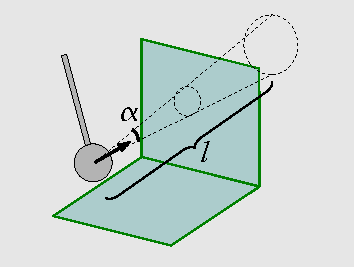
\includegraphics[width=3.5cm]{training}
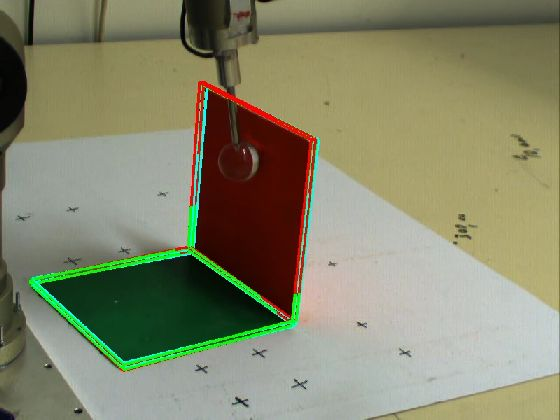
\includegraphics[width=3.5cm]{complex1}
}
\centerline{
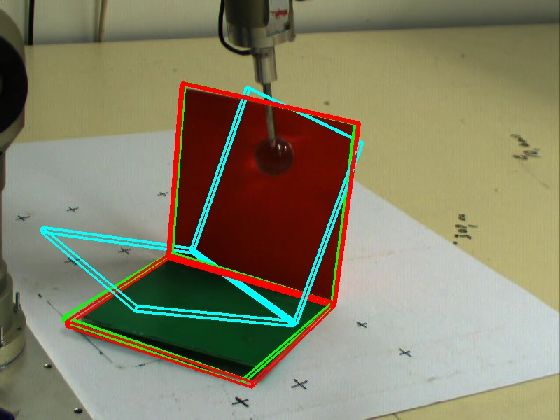
\includegraphics[width=3.5cm]{complex2}
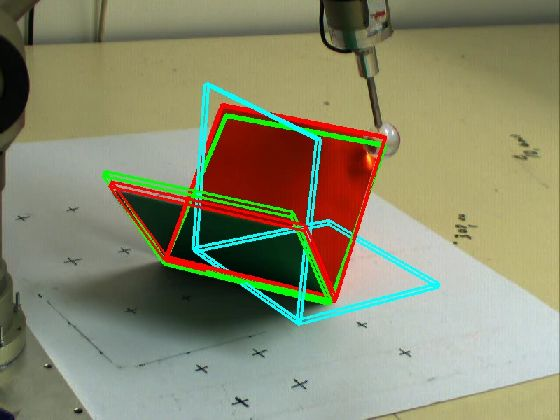
\includegraphics[width=3.5cm]{complex4}
}
\caption[Setup]{In all experiments the robot finger pushes in a straight-line of length $l$=25$\pm$5 cm within a cone of angle $\alpha$=20 deg toward an object (top left). The start point is randomised so that each region on the vertical face is equally likely to be pushed. The red wire-frame shows the output of the visual tracker, the green wire-frame the object pose predicted by the KDEF learner, and the blue wire-frame the prediction of the PhysX simulator.}
\label{fig:Setup}
\end{figure}

Local frames for environment contacts in the -GAE variants were fixed
by hand to the edges of objects. In test cases with new objects the
frames were again fixed by hand.  An item for future work is to
perform this process automatically.  All methods required parameter tuning. Model selection was performed in experiment P1 to establish reasonable parameter values, which were then used in experiments P2 and P3.  It was not possible to perform fully systematic optimisations for LWPR, KDE and KDEF due to the size of the parameter spaces.  Rather, subsets of the parameter space were selected by inspection and then explored using grid search.  Models were evaluated on a separate hold-out set, of the same size as the test set. Model selection by full grid search was performed for the following parameters of the PhysX simulator: static friction, dynamic friction and the coefficient of restitution. The full set of parameters is given in Table~\ref{tab:physx}, leading to 125 different parameter combinations being tried for PhysX for each training object. PhysX has access to full mesh and contact information. Parameter search for the KDE methods was performed for the bandwidth of the kernels, with three values tried. For the KDE and LWPR methods, in addition to model selection the three different parameterisations (Gauss-Euler (e), Gauss-Quaternion (q), Von-Mises-Fisher-Quat (v)) of rotations for the density estimation method were studied in experiment P1, and subsequently the best solution was used in experiments P2 and P3. For LWPR we used the Euler parameterisation throughout experiments P1, P2 and P3. For experiment P1 we performed 10-fold cross-validation. The sizes of the training and test sets are stated in the method for each experiment. For transfer learning experiments P2 and P3, disjoint training and test sets were used. For clarity a complete set of acronyms for the algorithm-information combinations is given in Table~\ref{tab:algs}. 
\begin{table}[b]
\begin{center}
\begin{tabular}{|l|l|l|l|l|l|}\hline
Parameter & \multicolumn{5}{|c|}{Values} \\ \hline
restitution & 0.125 & 0.1875 & 0.25 &  0.375 & 0.5\\ \hline
static friction & 0.25 & 0.3125 & 0.5 & 0.75 & 1.0  \\ \hline
dynamic friction & 0.25 & 0.3125 & 0.5 & 0.75 & 1.0\\ \hline
\end{tabular}
\caption{Parameter settings for optimisation of PhysX. \label{tab:physx}}
\end{center}
\end{table}

\begin{table}[b]
\begin{center}
\begin{tabular}{|l|l|l|l|}\hline
 & \multicolumn{3}{|c|}{Information} \\ \hline
Predictor & G & G+A & G+A+E \\ \hline
LWPR & LWPR-G& LWPR-GA & LWPR-GAE \\ \hline
KDE & KDE-G & KDE-GA & KDE-GAE \\ \hline
KDEF & KDEF-G & KDEF-GA & KDEF-GAE \\ \hline
PhysX & n/a & n/a & n/a \\ \hline
\end{tabular}
\caption{Algorithm-information variants. \label{tab:algs}}
\end{center}
\end{table}
%%%%%%%%%%%%%%%%%%%%%%%%%%%%%%%%%%%%%%%%%%%%%%%%%%%%%%%%%%%%%%%%%%%%%%%
\subsection{Performance measure}\label{sec:Experiment.Performance}

In all experiments with real objects, predicted trajectories were evaluated against the visual tracked object pose. The tracker does not provide perfect ground-truth, yielding errors of $\pm$2mm. Prediction performance is evaluated as follows.

At any particular time step, $t$, a large number, $N$, of randomly chosen points $p_{n}^{1,t}$, where $n=1 \ldots N$, are rigidly attached to an object at the ground-truth pose, and the corresponding points $p_{n}^{2,t}$ to an object at the predicted pose. At time step $t$, an average error $E_t$ can now be defined as the mean of displacements between points on the object at the predicted pose and points on the object at the ground-truth pose:
\begin{equation}
E_t = \frac{1}{N} \mathop{\sum}_{n=1 \ldots N}|p_{n}^{2,t}-p_{n}^{1,t}|
\label{eq:defn_Rt}
\end{equation}
Note that for each push action, we predict approximately 150
consecutive steps into the future, with no recursive filtering or
corrector steps, hence it is expected that errors will grow with range
from the initial object pose. We therefore find it more meaningful to
normalise all errors with respect to an ``average range'', $R_t$, of
the object from its starting position, defined as:
\begin{equation}
R_t = \frac{1}{N} \mathop{\sum}_{n=1 \ldots N}|p_{n}^{1,t}-p_{n}^{1,0}|
\label{eq:defn_Et}
\end{equation}
For a test data set, consisting of $K$ robotic pushes, each of which breaks down into many consecutive predictions over $T$ time steps, we can now define average error and normalised average error. Note that the normalised error measure necessarily has no units.
\begin{align}
E_{av} &= \frac{1}{K} \mathop{\sum}_{k=1}^{K} \frac{1}{T} \mathop{\sum}_{t=1}^{T} E_t,
&E_{av}^{norm} &= \frac{1}{K} \mathop{\sum}_{k=1}^{K} \frac{1}{T} \mathop{\sum}_{t=1}^{T} \frac{E_t}{R_t}
\label{eq:Error1}
\end{align}


\begin{figure*}[t]
\centerline{
\includegraphics[width=0.8\textwidth]{./P1-graphs}
%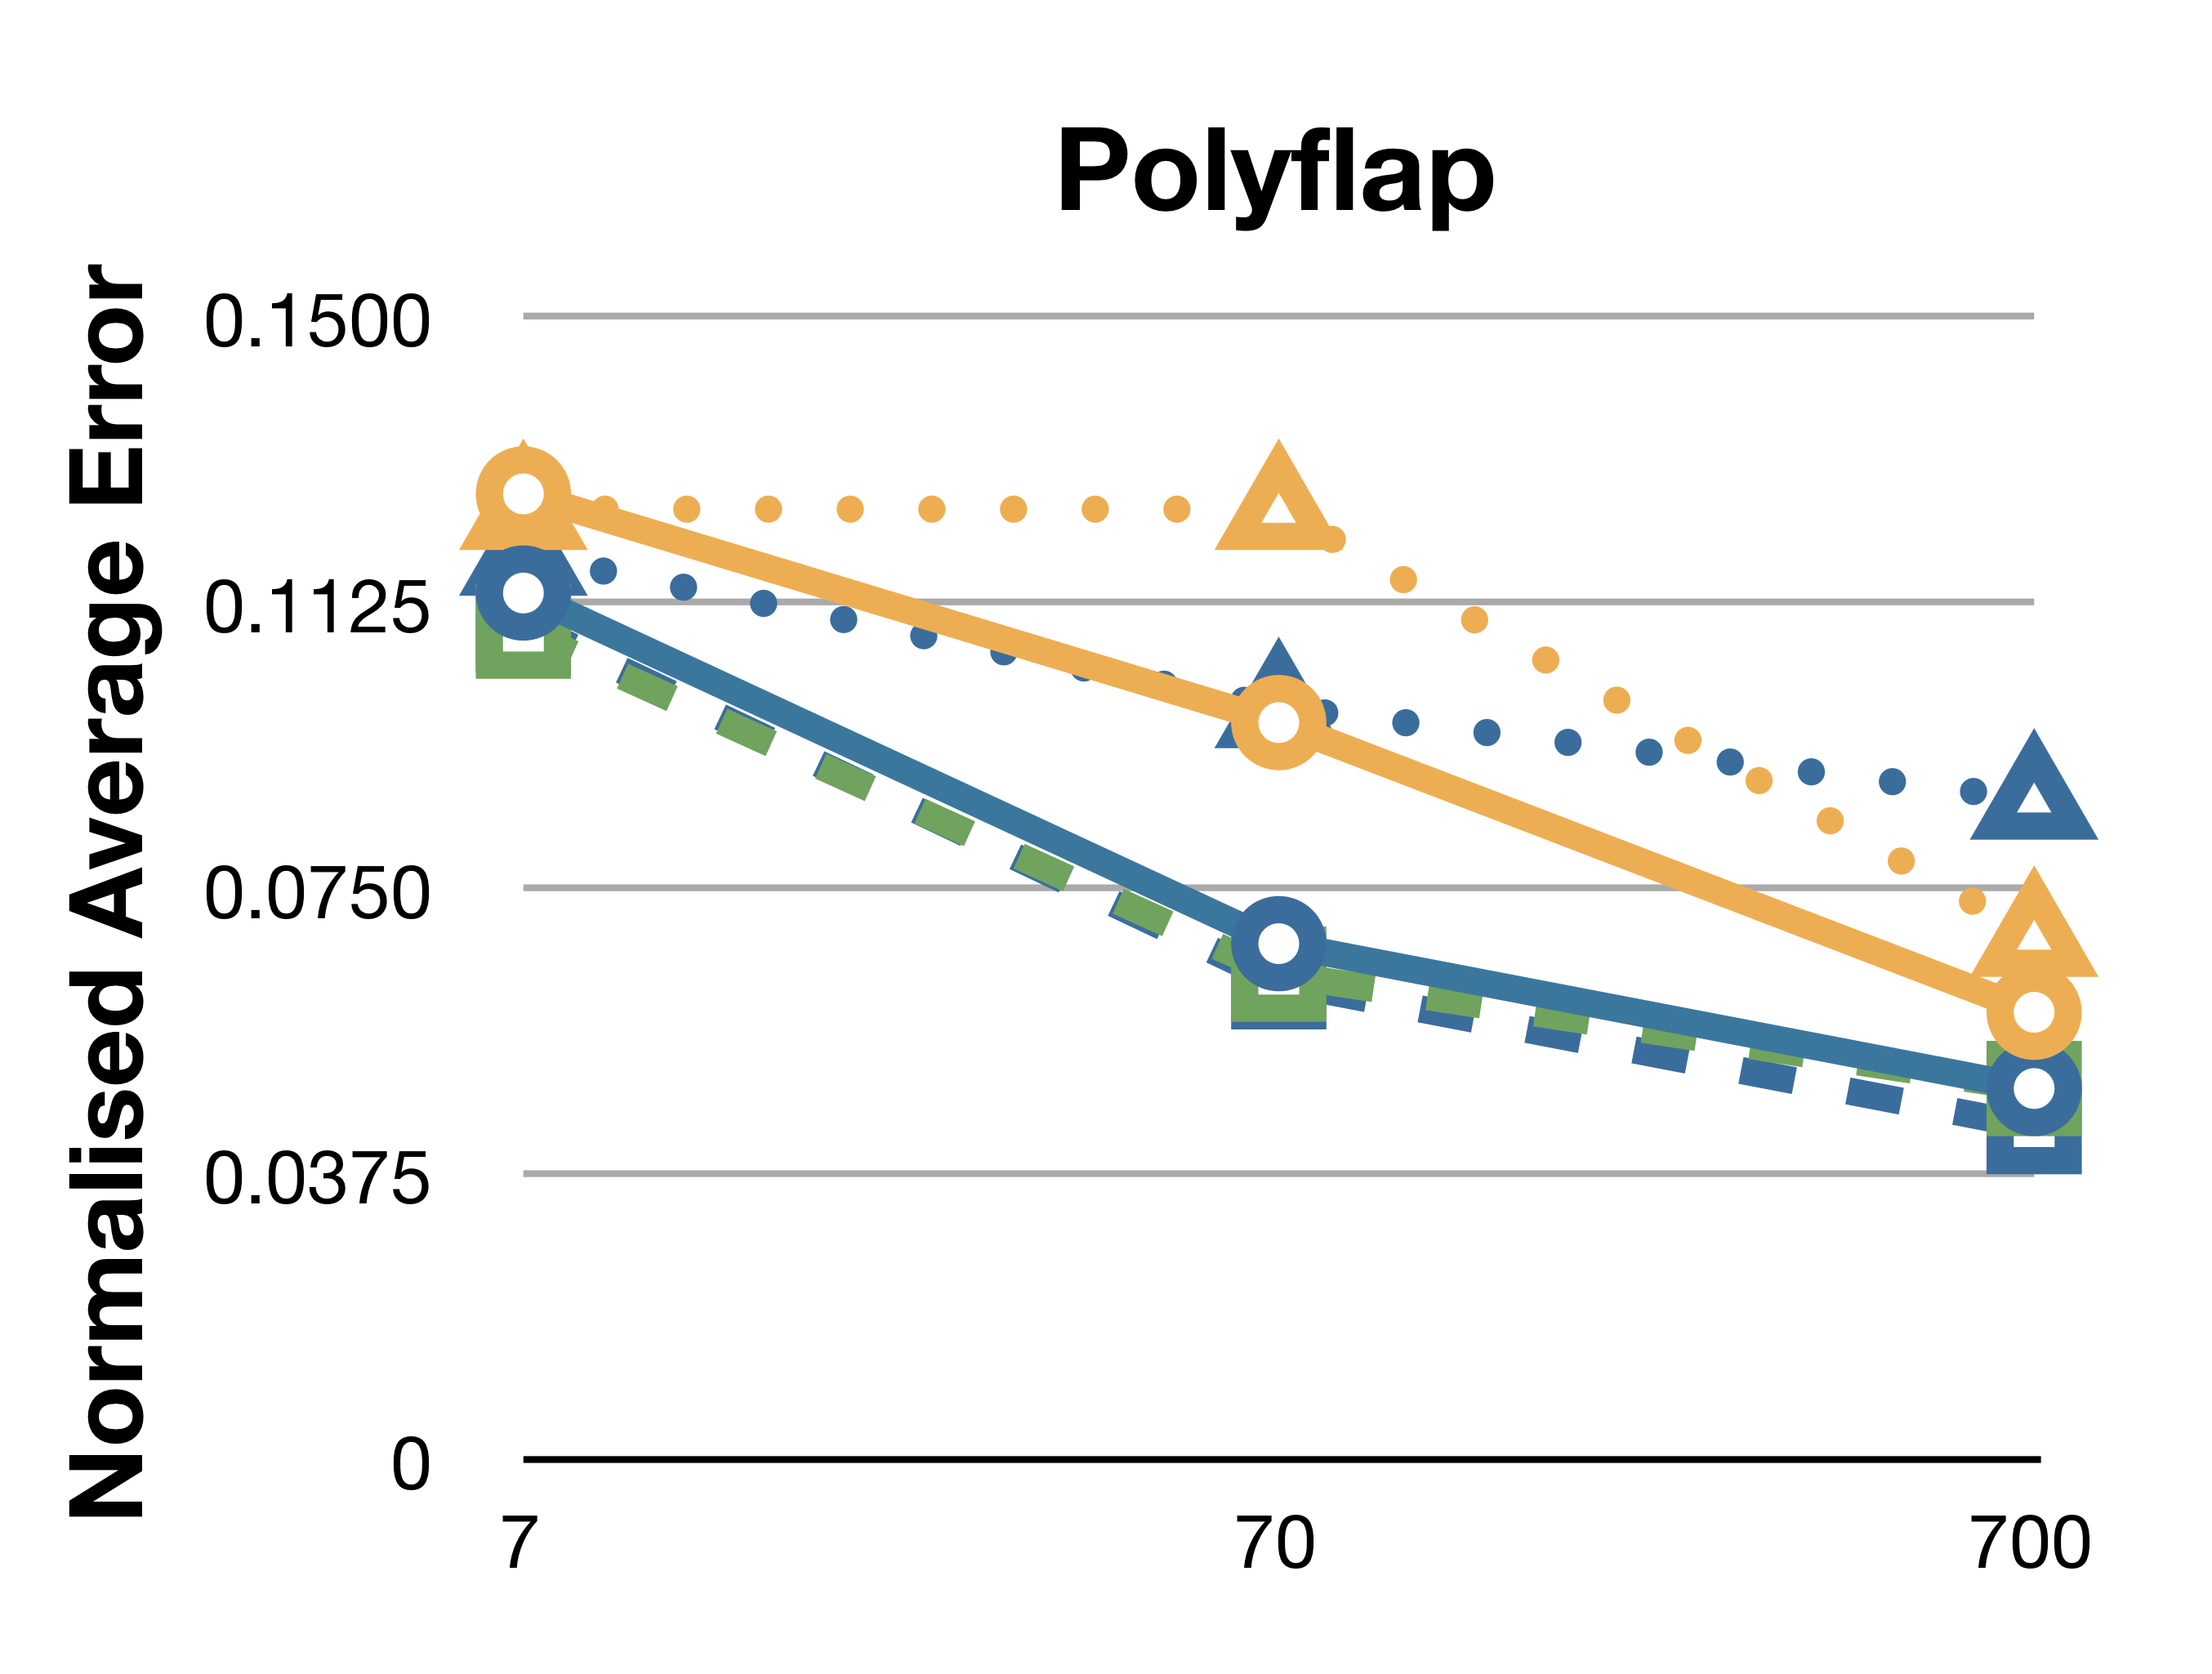
\includegraphics[width=0.45\columnwidth]{./L1av_graph}
%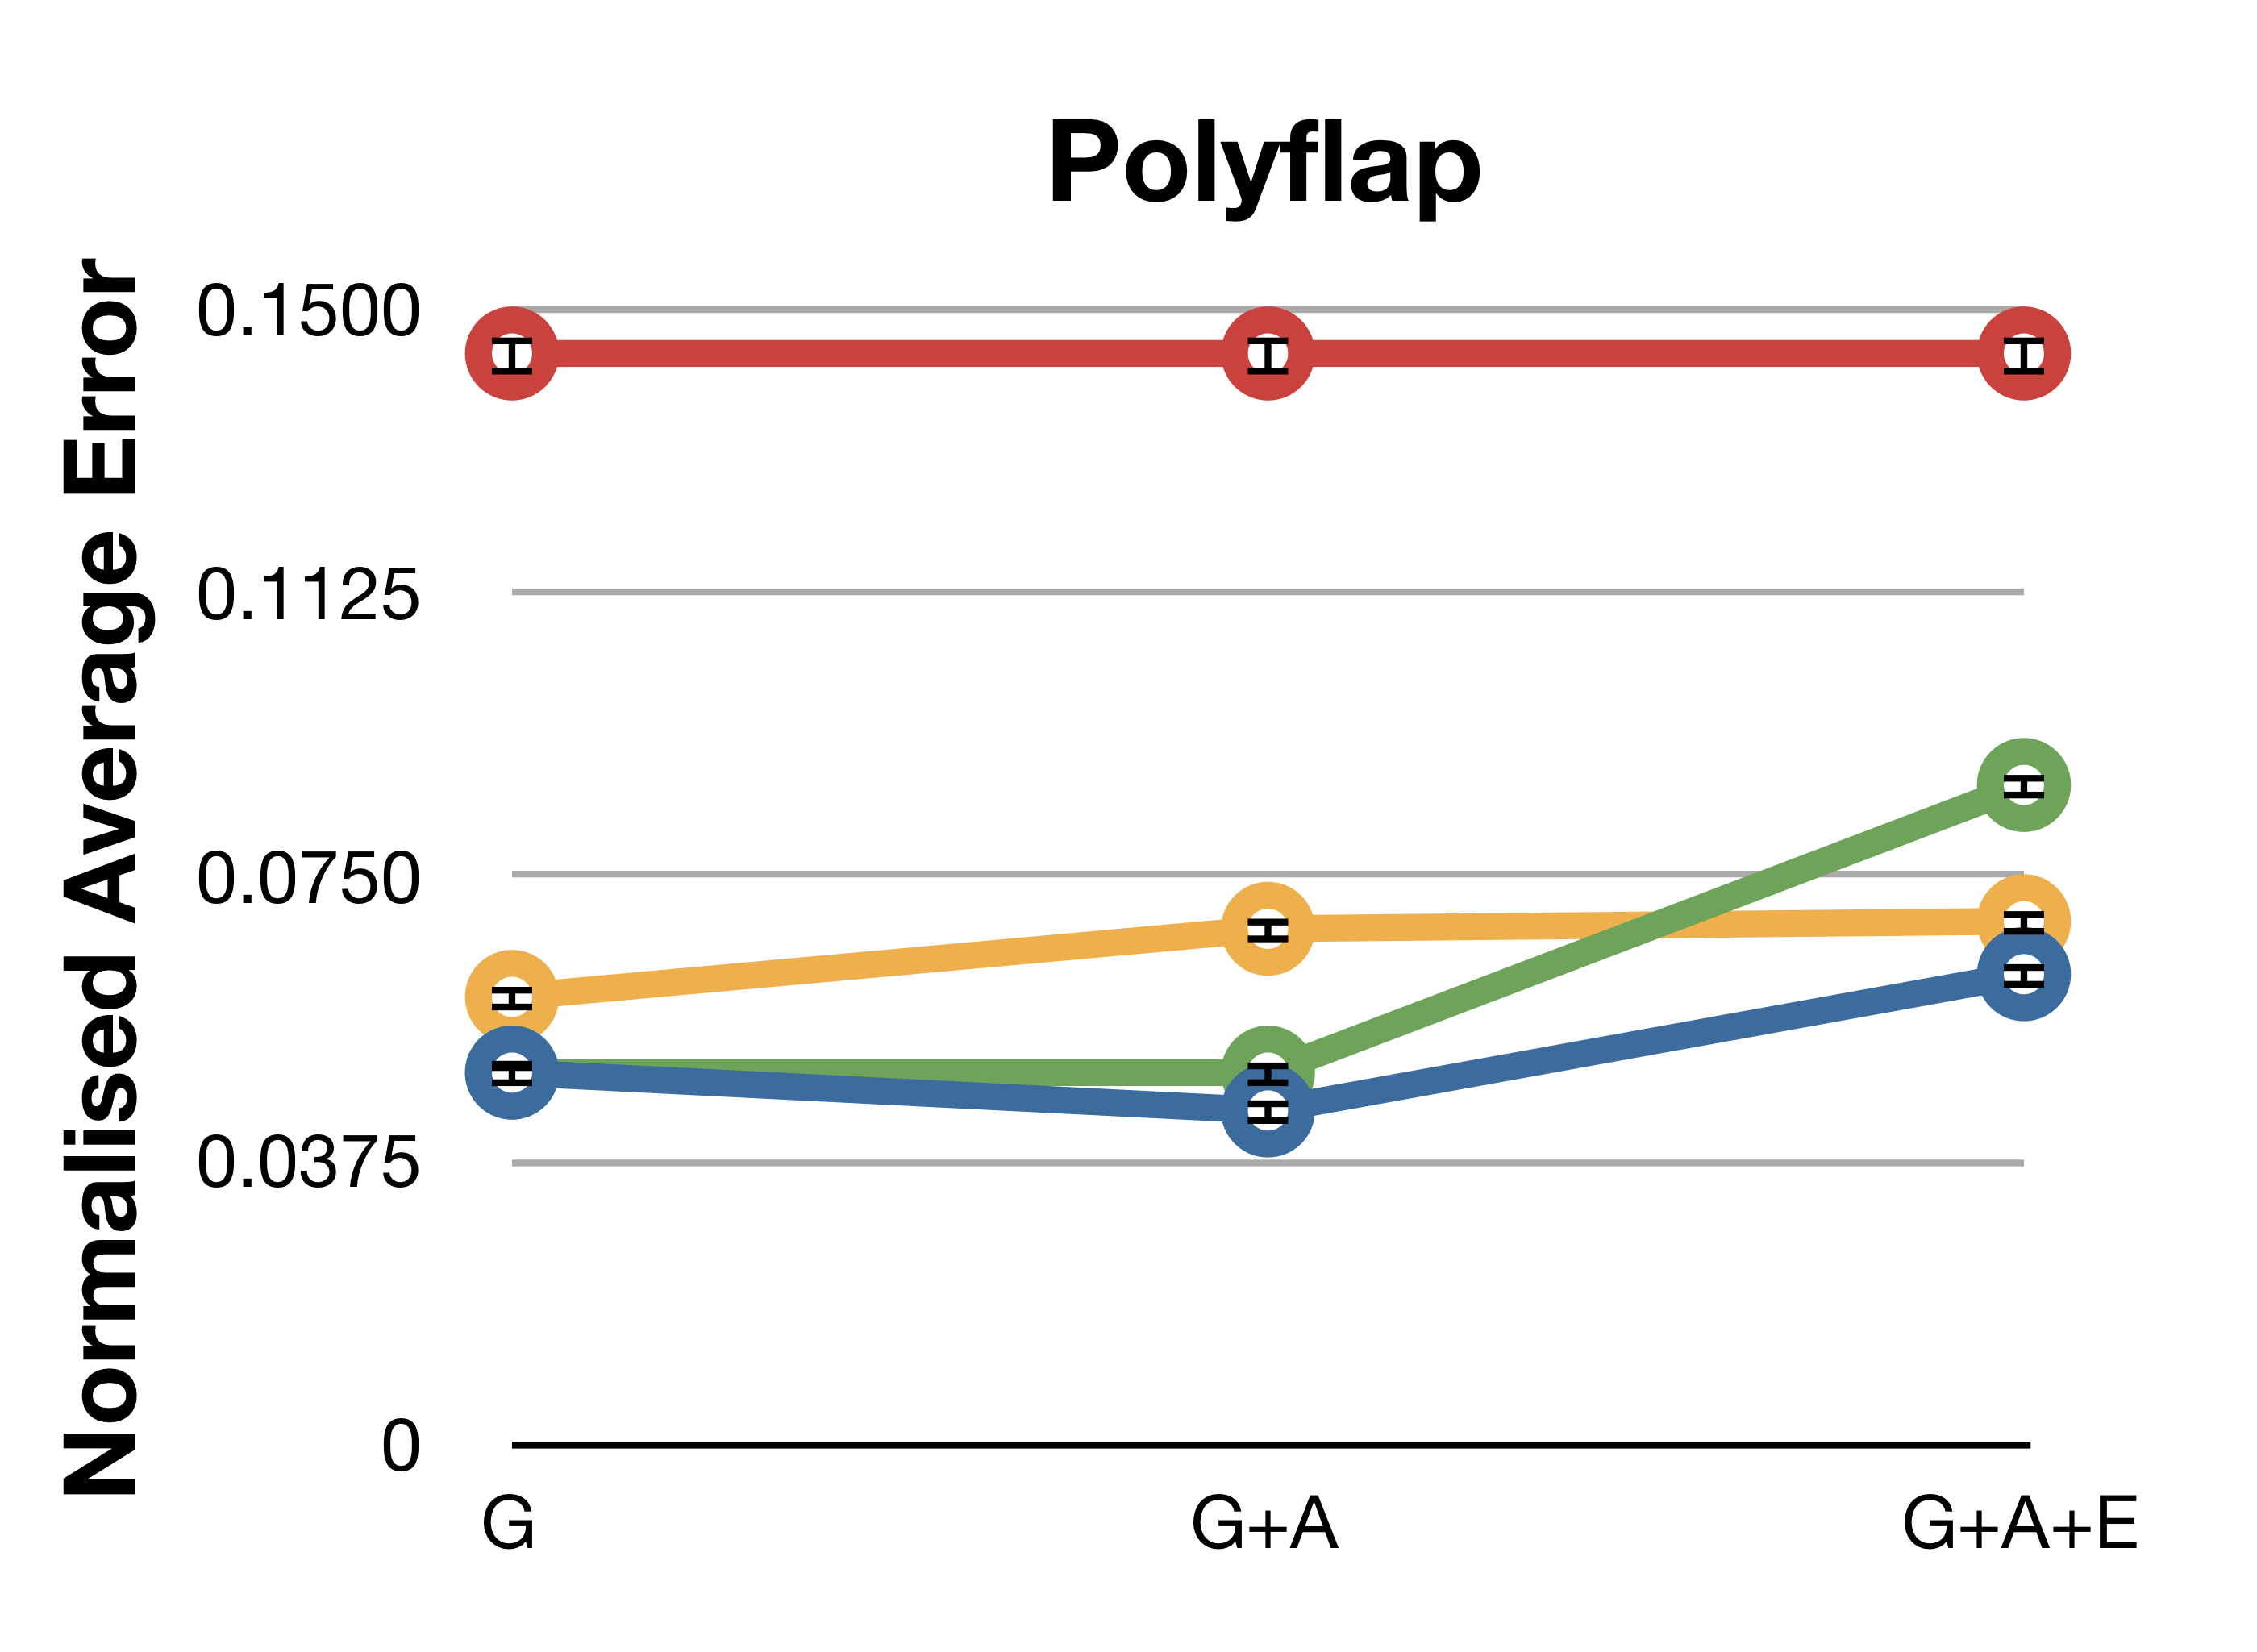
\includegraphics[width=0.45\columnwidth]{./L1av_graph_polyflap}
%}
%\centerline{
%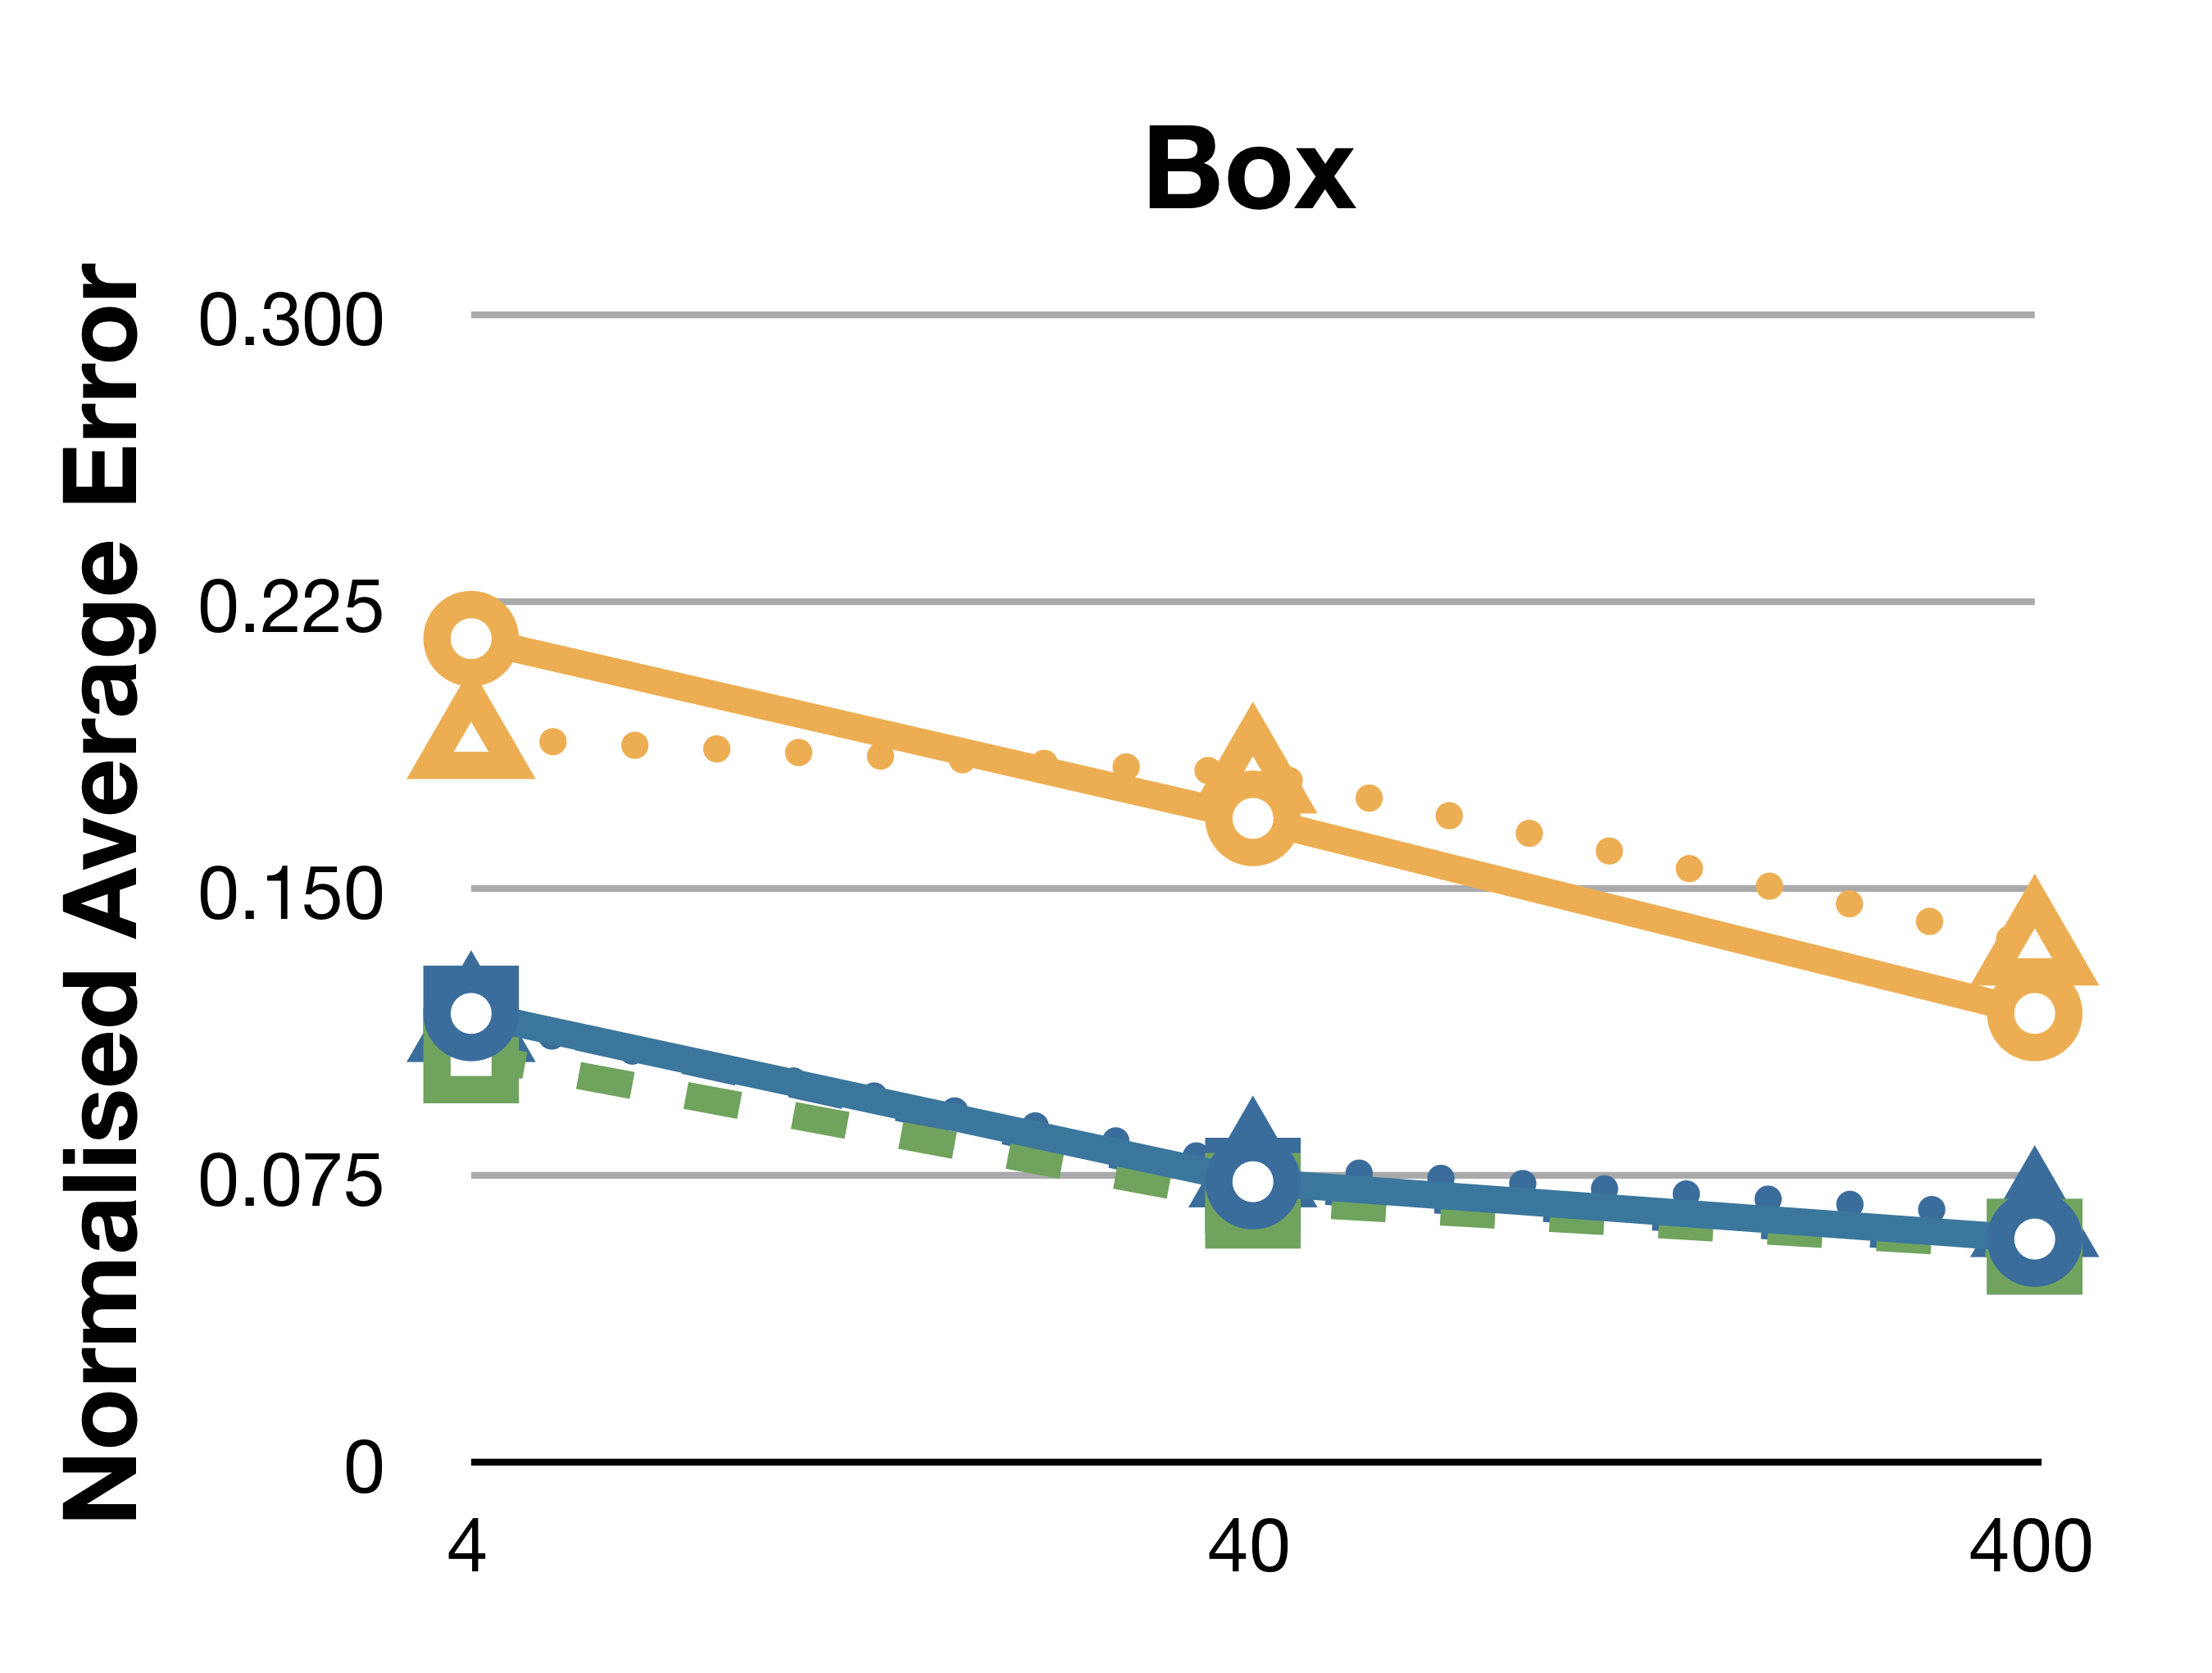
\includegraphics[width=0.45\columnwidth]{./L2av_graph}
%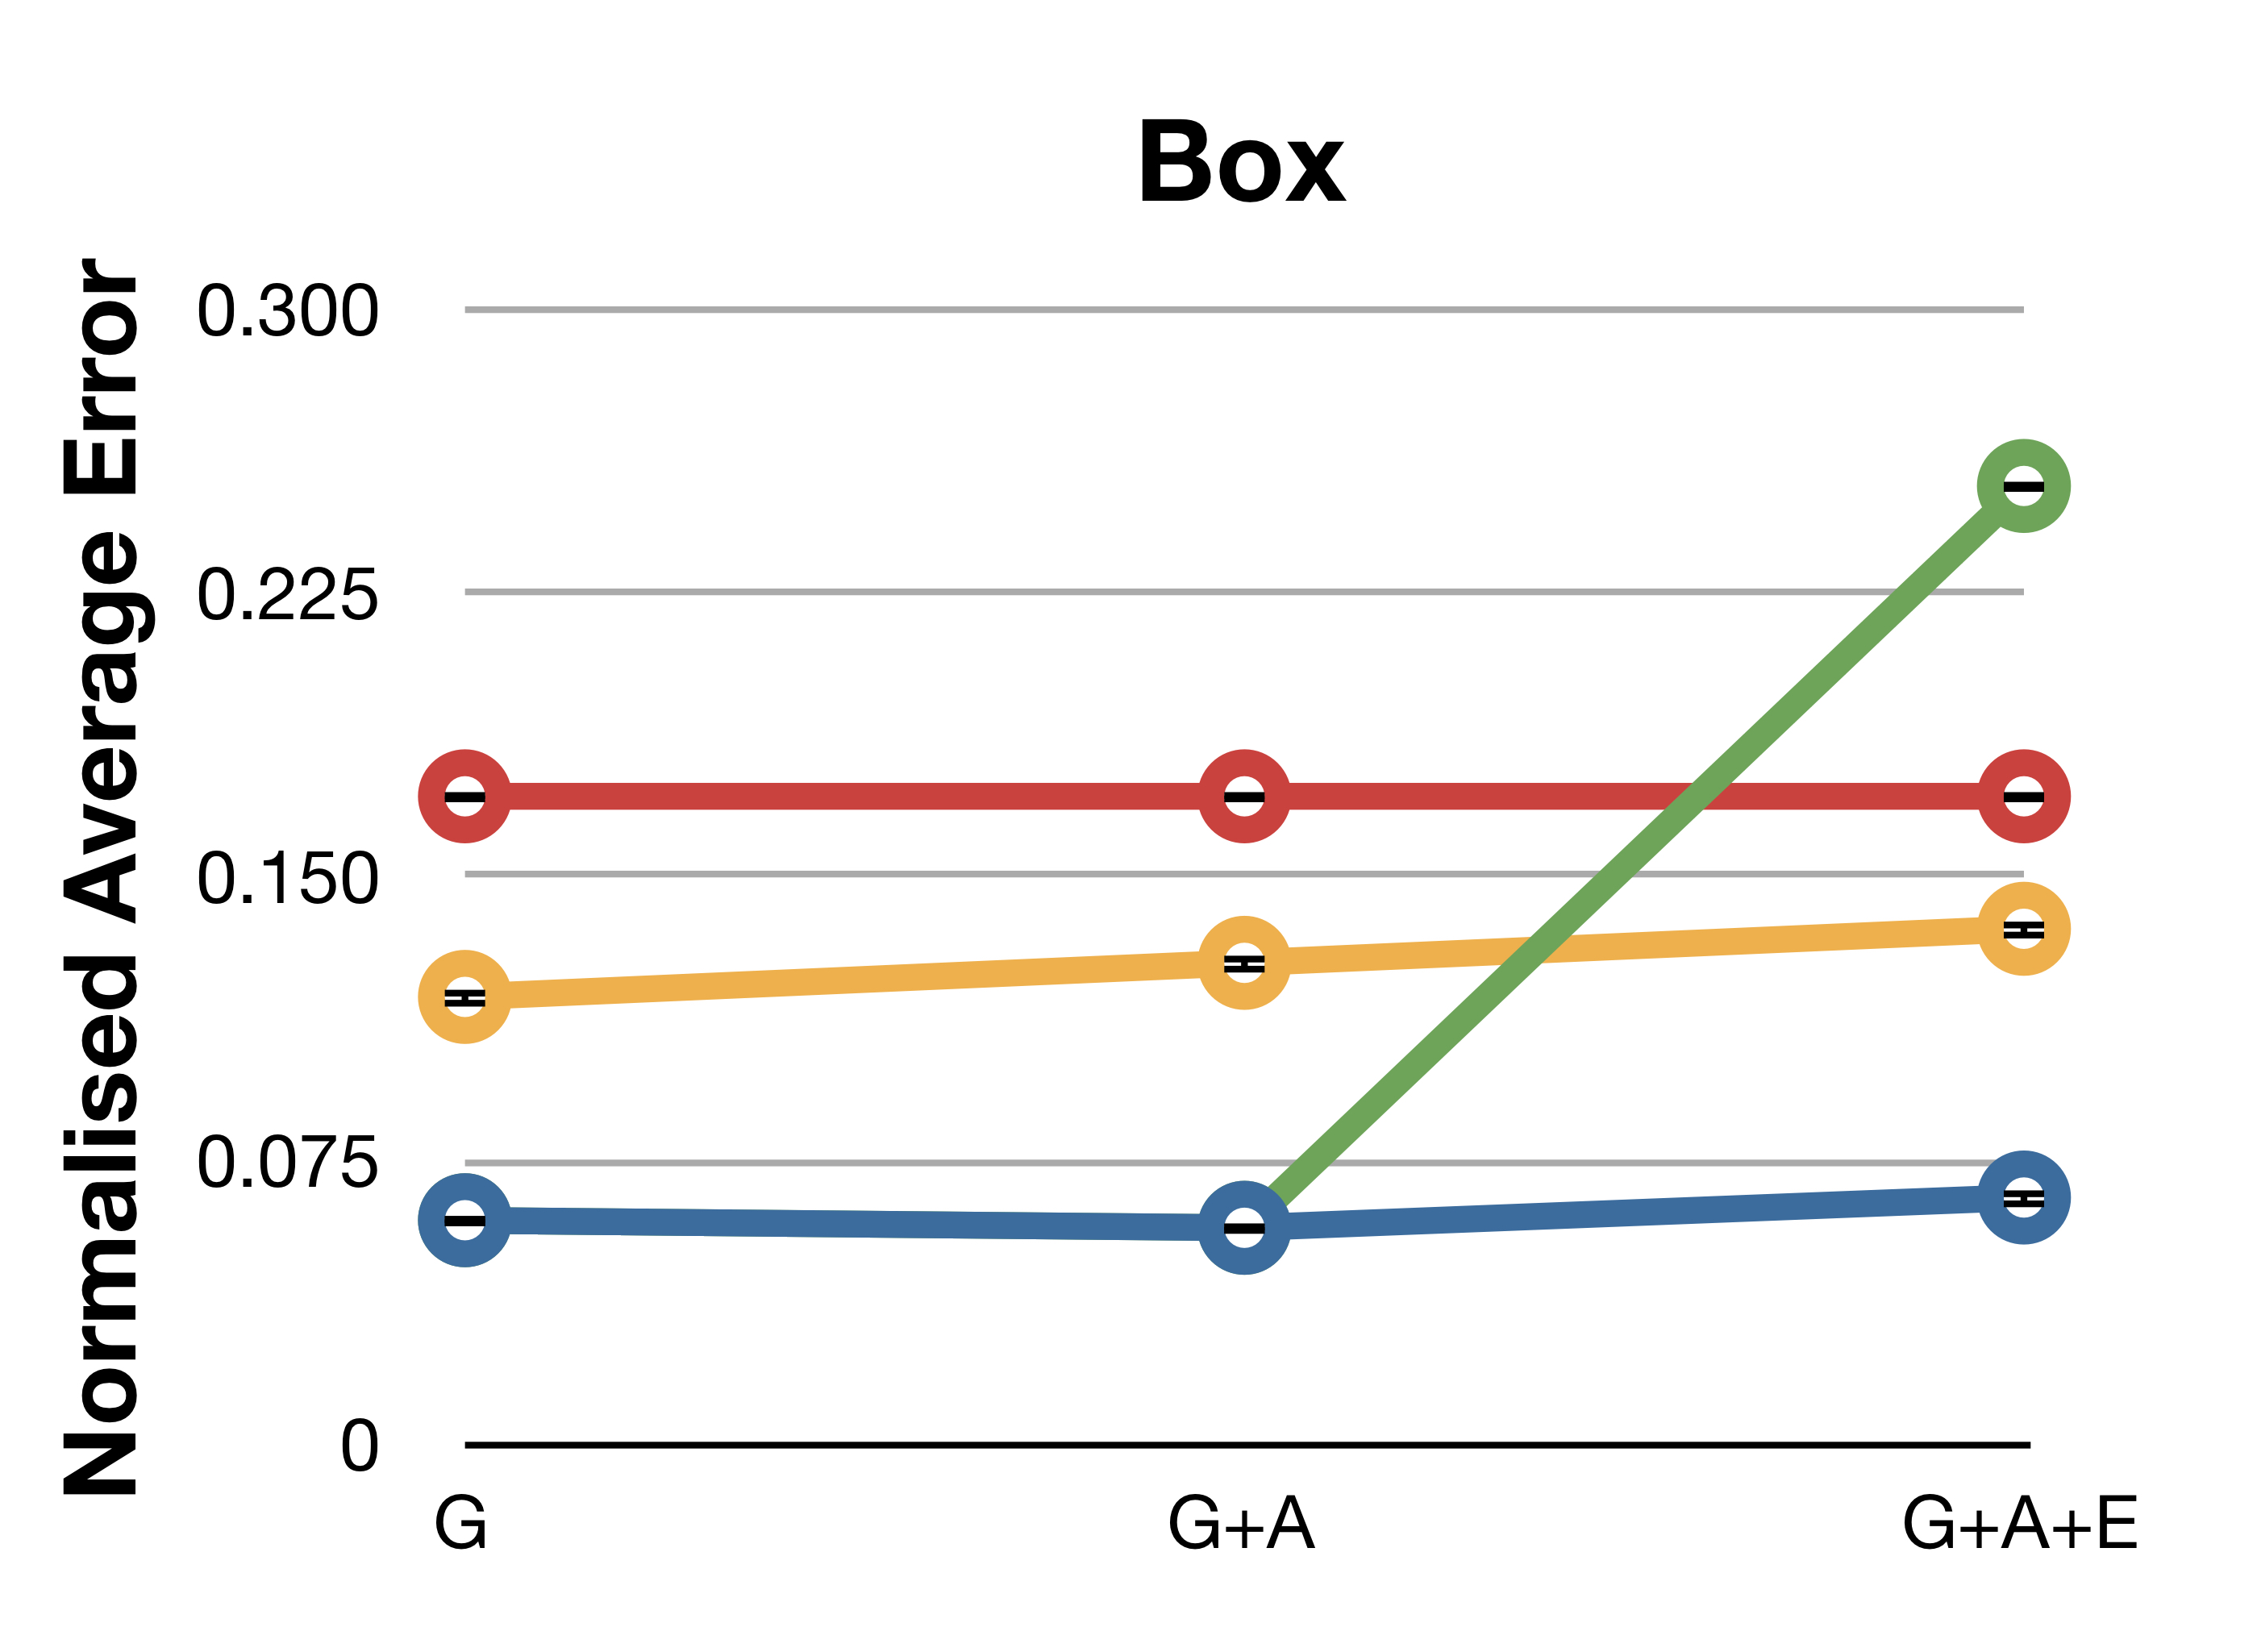
\includegraphics[width=0.45\columnwidth]{./L1av_graph_box}
%}
%\centerline{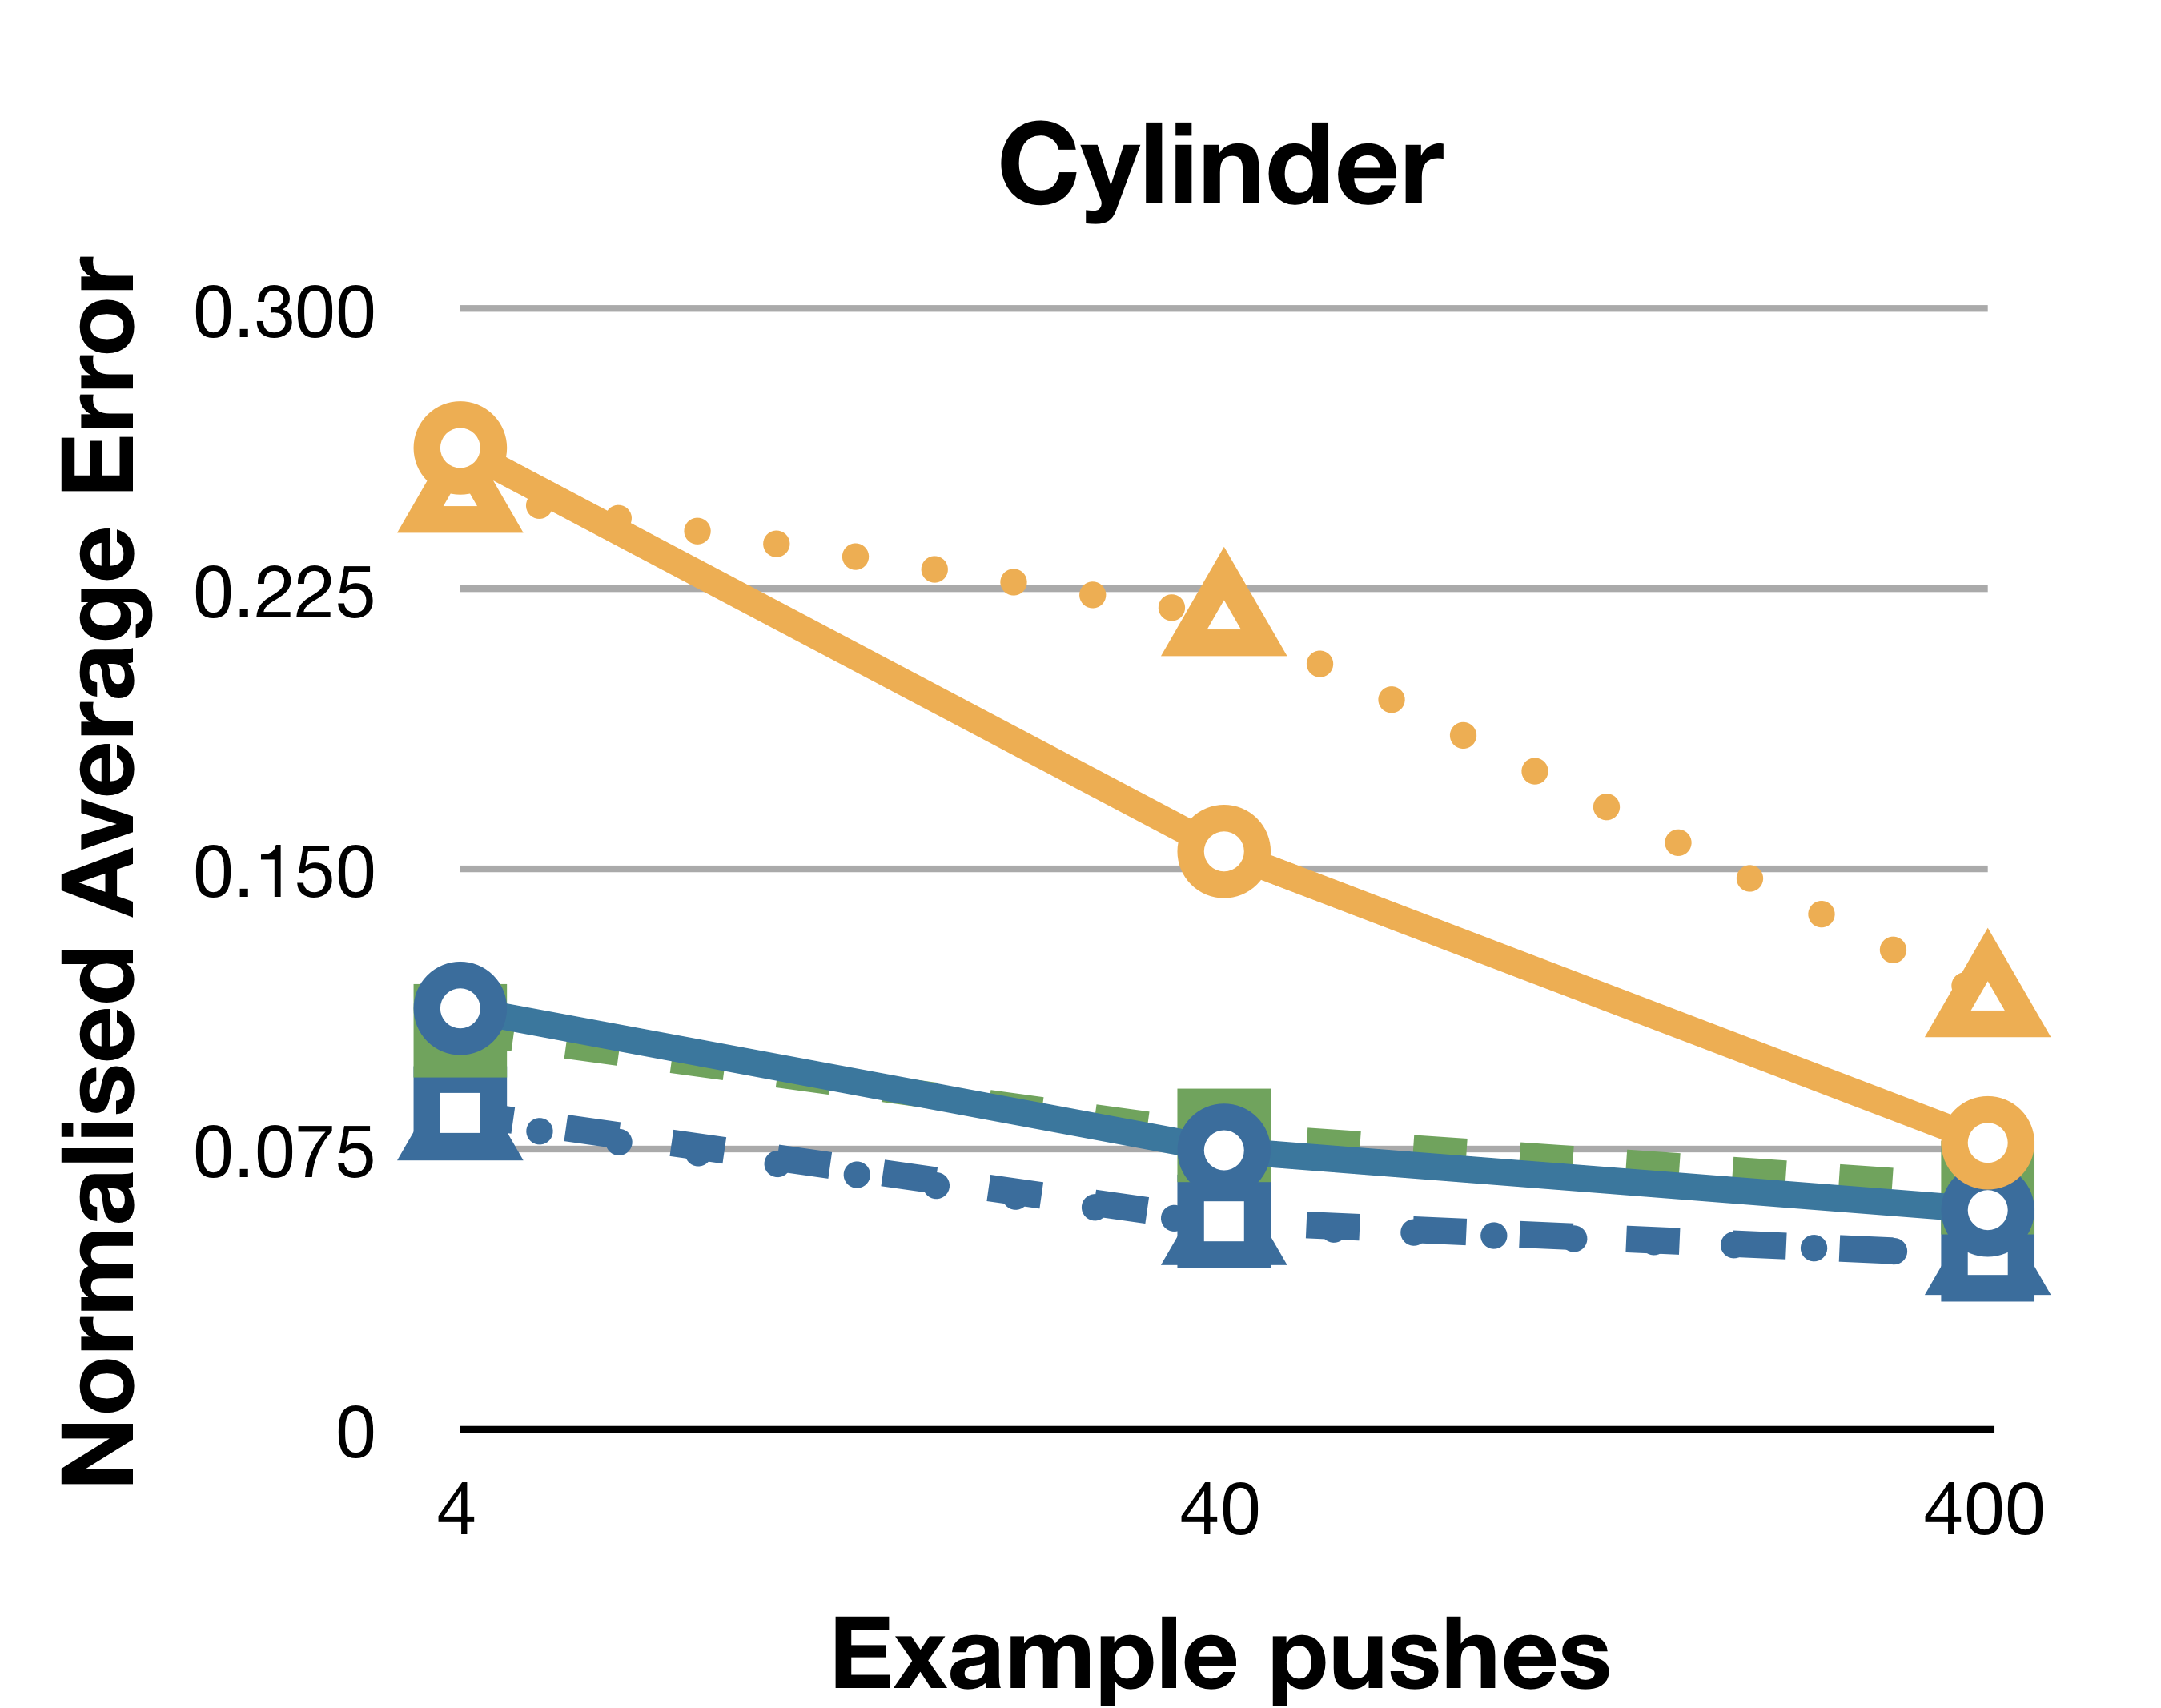
\includegraphics[width=0.45\columnwidth]{./L3av_graph}
%                 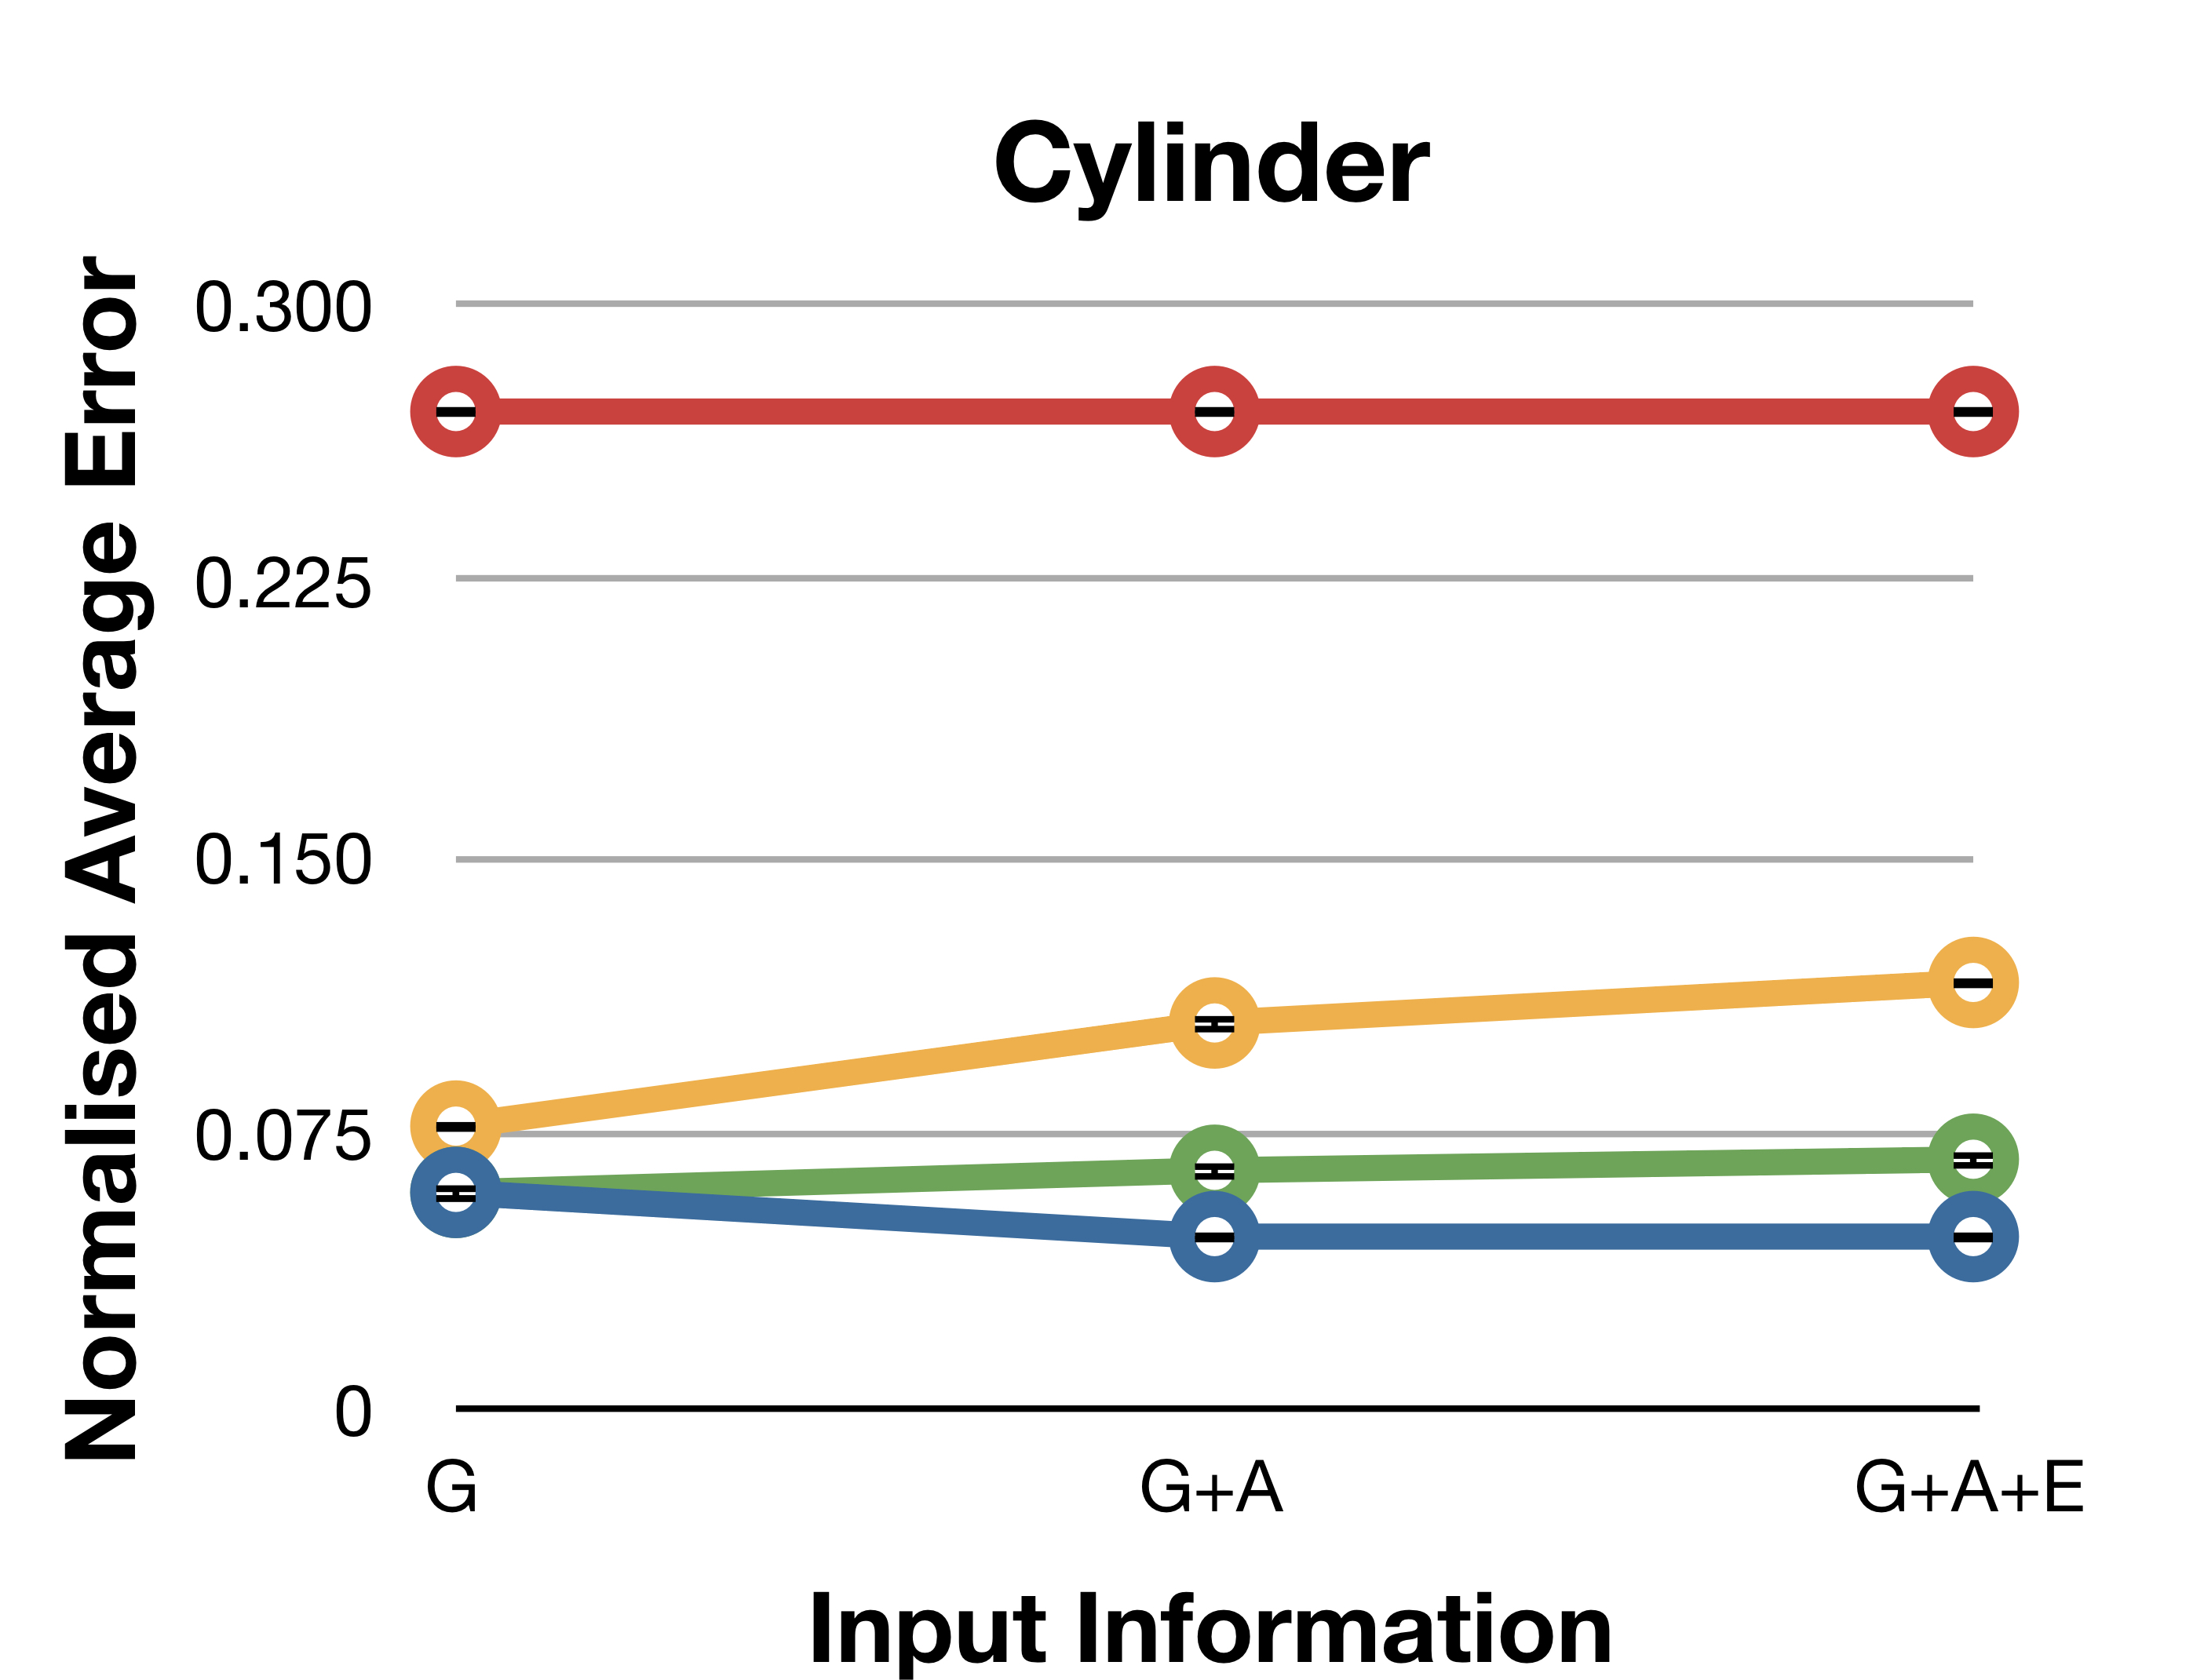
\includegraphics[width=0.45\columnwidth]{./L1av_graph_cylinder}
%}
%\centerline{
\includegraphics[width=\linewidth]{./L1_convergence_graph_key}
}
\vspace{-1mm}
\caption{Experiment P1: Convergence of a selection of learning
  algorithm-information combinations (left column). Change in normalised average prediction errors with varying input information (right column). G - global information; A - agent-object information; E - object-environment information. Standard error bars are shown in black, in most cases these are very small and fall within the symbol for each data point. We show error bars for all data points except for the learning convergence graph shown here.}
\label{fig:Lgraphs}
\end{figure*}


\section{Results}\label{sec:Results}

\subsection{Experiment P1: Action Interpolation}\label{sec:Results.Learning}

In Experiment P1 the robot applied a set of random pushes to a
polyflap, a box and a cylinder respectively. All the algorithm
variants in Table~\ref{tab:algs} were trained and tested. Model
selection was performed for all algorithm-information combinations including PhysX. Ten fold cross-validation was performed for all algorithms. The density estimation techniques were studied with all three parameterisations of rotation. Training (and testing) sets were 200 (25) pushes (cylinder), 400 (50) pushes (box) and 700 (90) pushes (polyflap). Figure~\ref{fig:Lgraphs} (left column) shows convergence of the best learning algorithms. Figure~\ref{fig:Lgraphs} (right column) shows how performance varies with input information for the best parameterisations of all the algorithms. Table~\ref{tab:PerformanceTableL1av} shows the results of model selection on the different parameterisations for KDE. Image sequences of predicted vs actual trajectories are shown in (Figure~\ref{fig:ExperimentL2}). For the simulation experiments on non-planar surfaces, 900 (100) pushes of a cylinder in two different starting positions (upright and on its side) were made. For this simulated experiment we only used factored KDE  with the Gaussian-quaternion parameterisation, on the basis that this was the best performing setup for the real experiments. 

\begin{figure}[t]
\centerline{
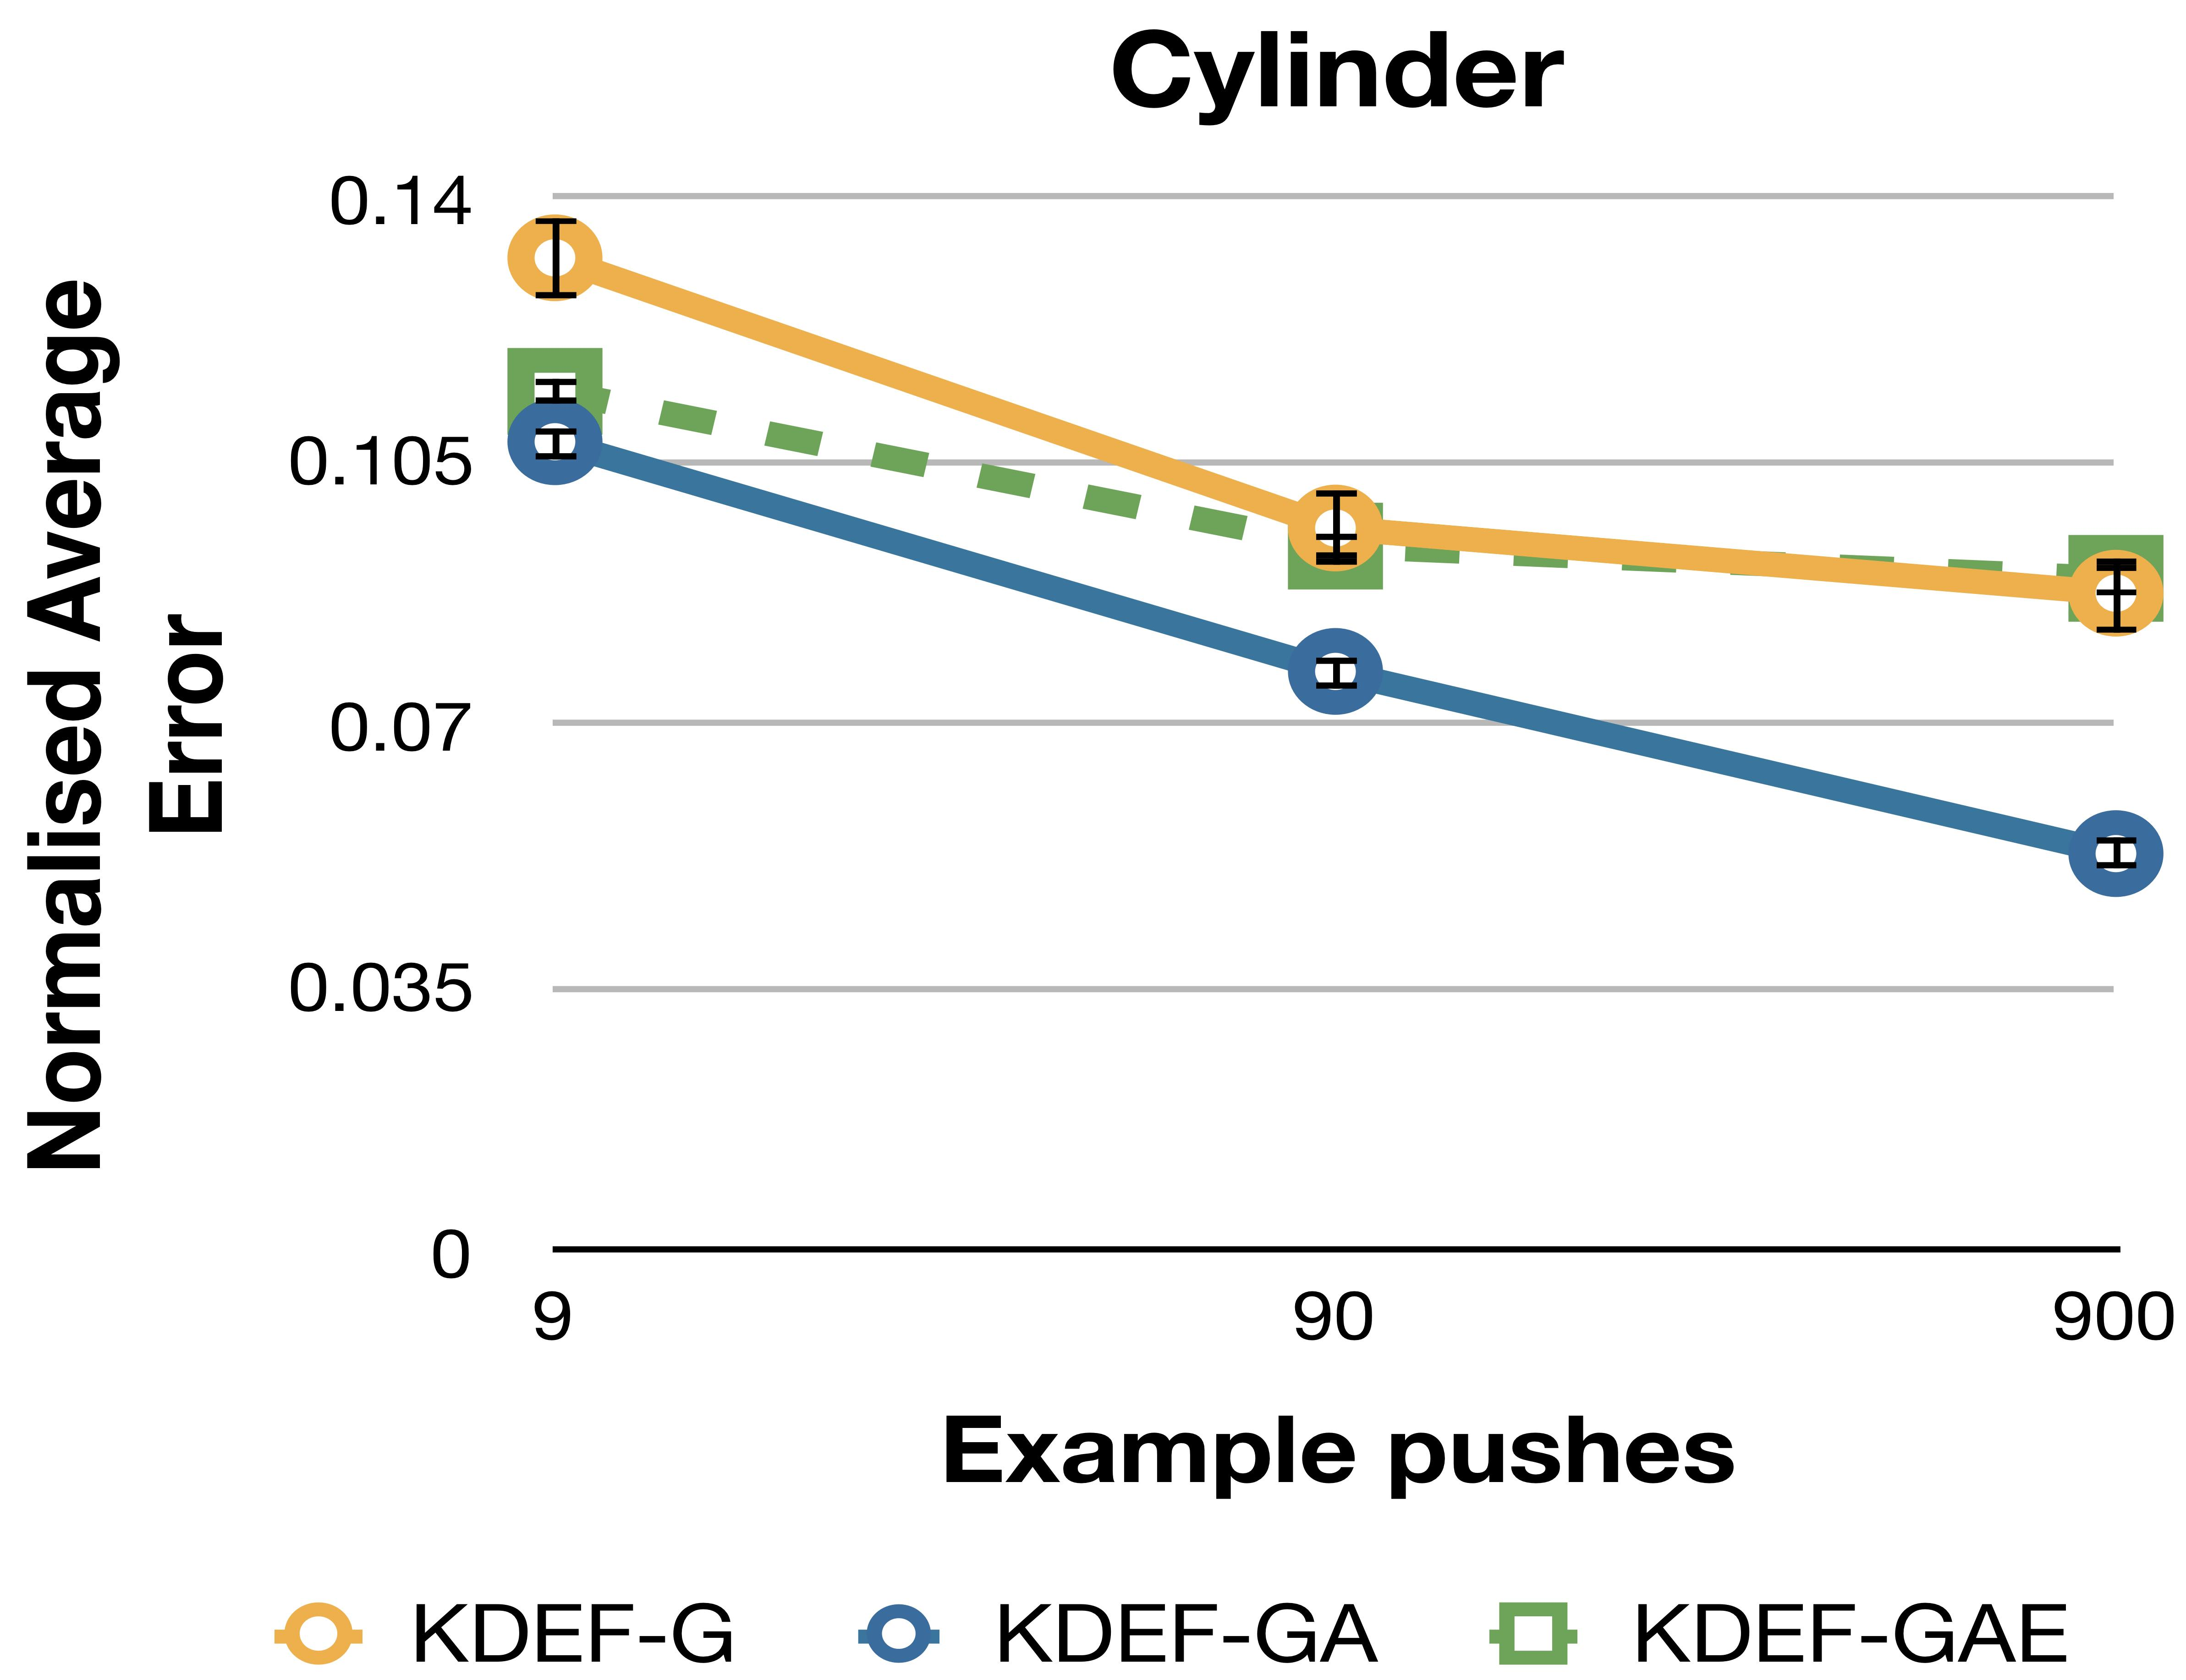
\includegraphics[width=0.9\columnwidth]{./L1av-graph-cyl-sim}
%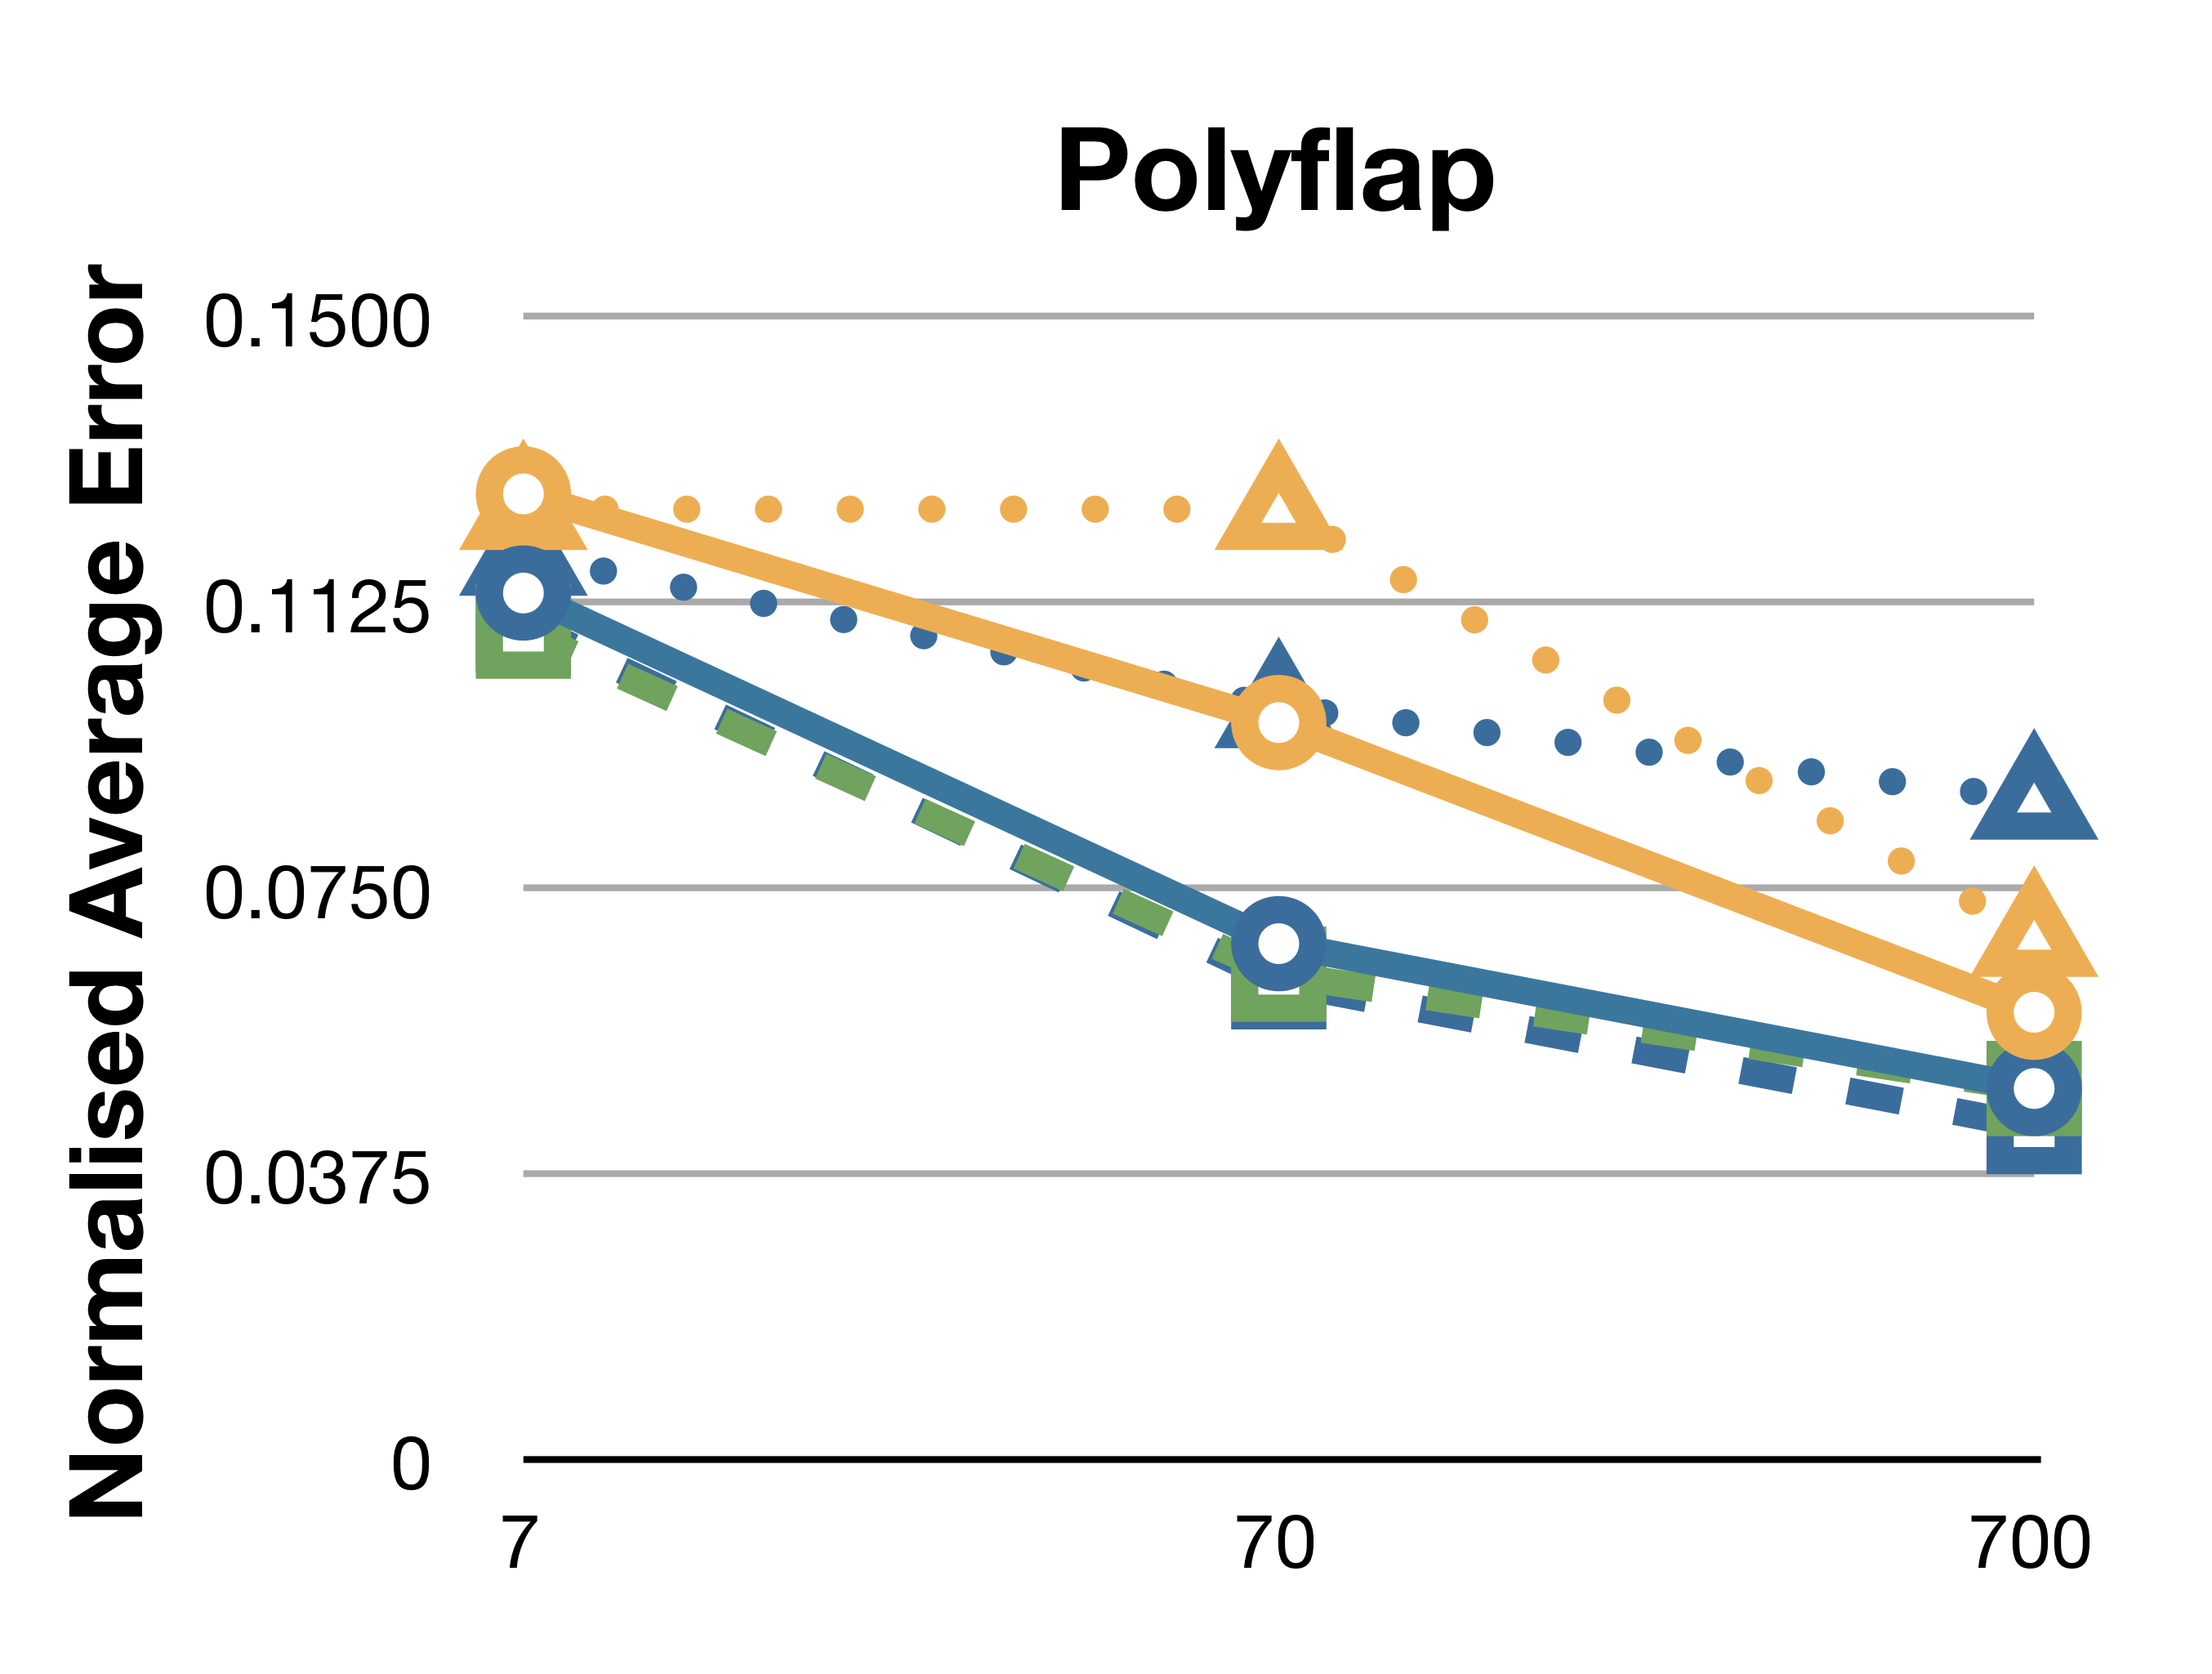
\includegraphics[width=0.45\columnwidth]{./L1av_graph}
%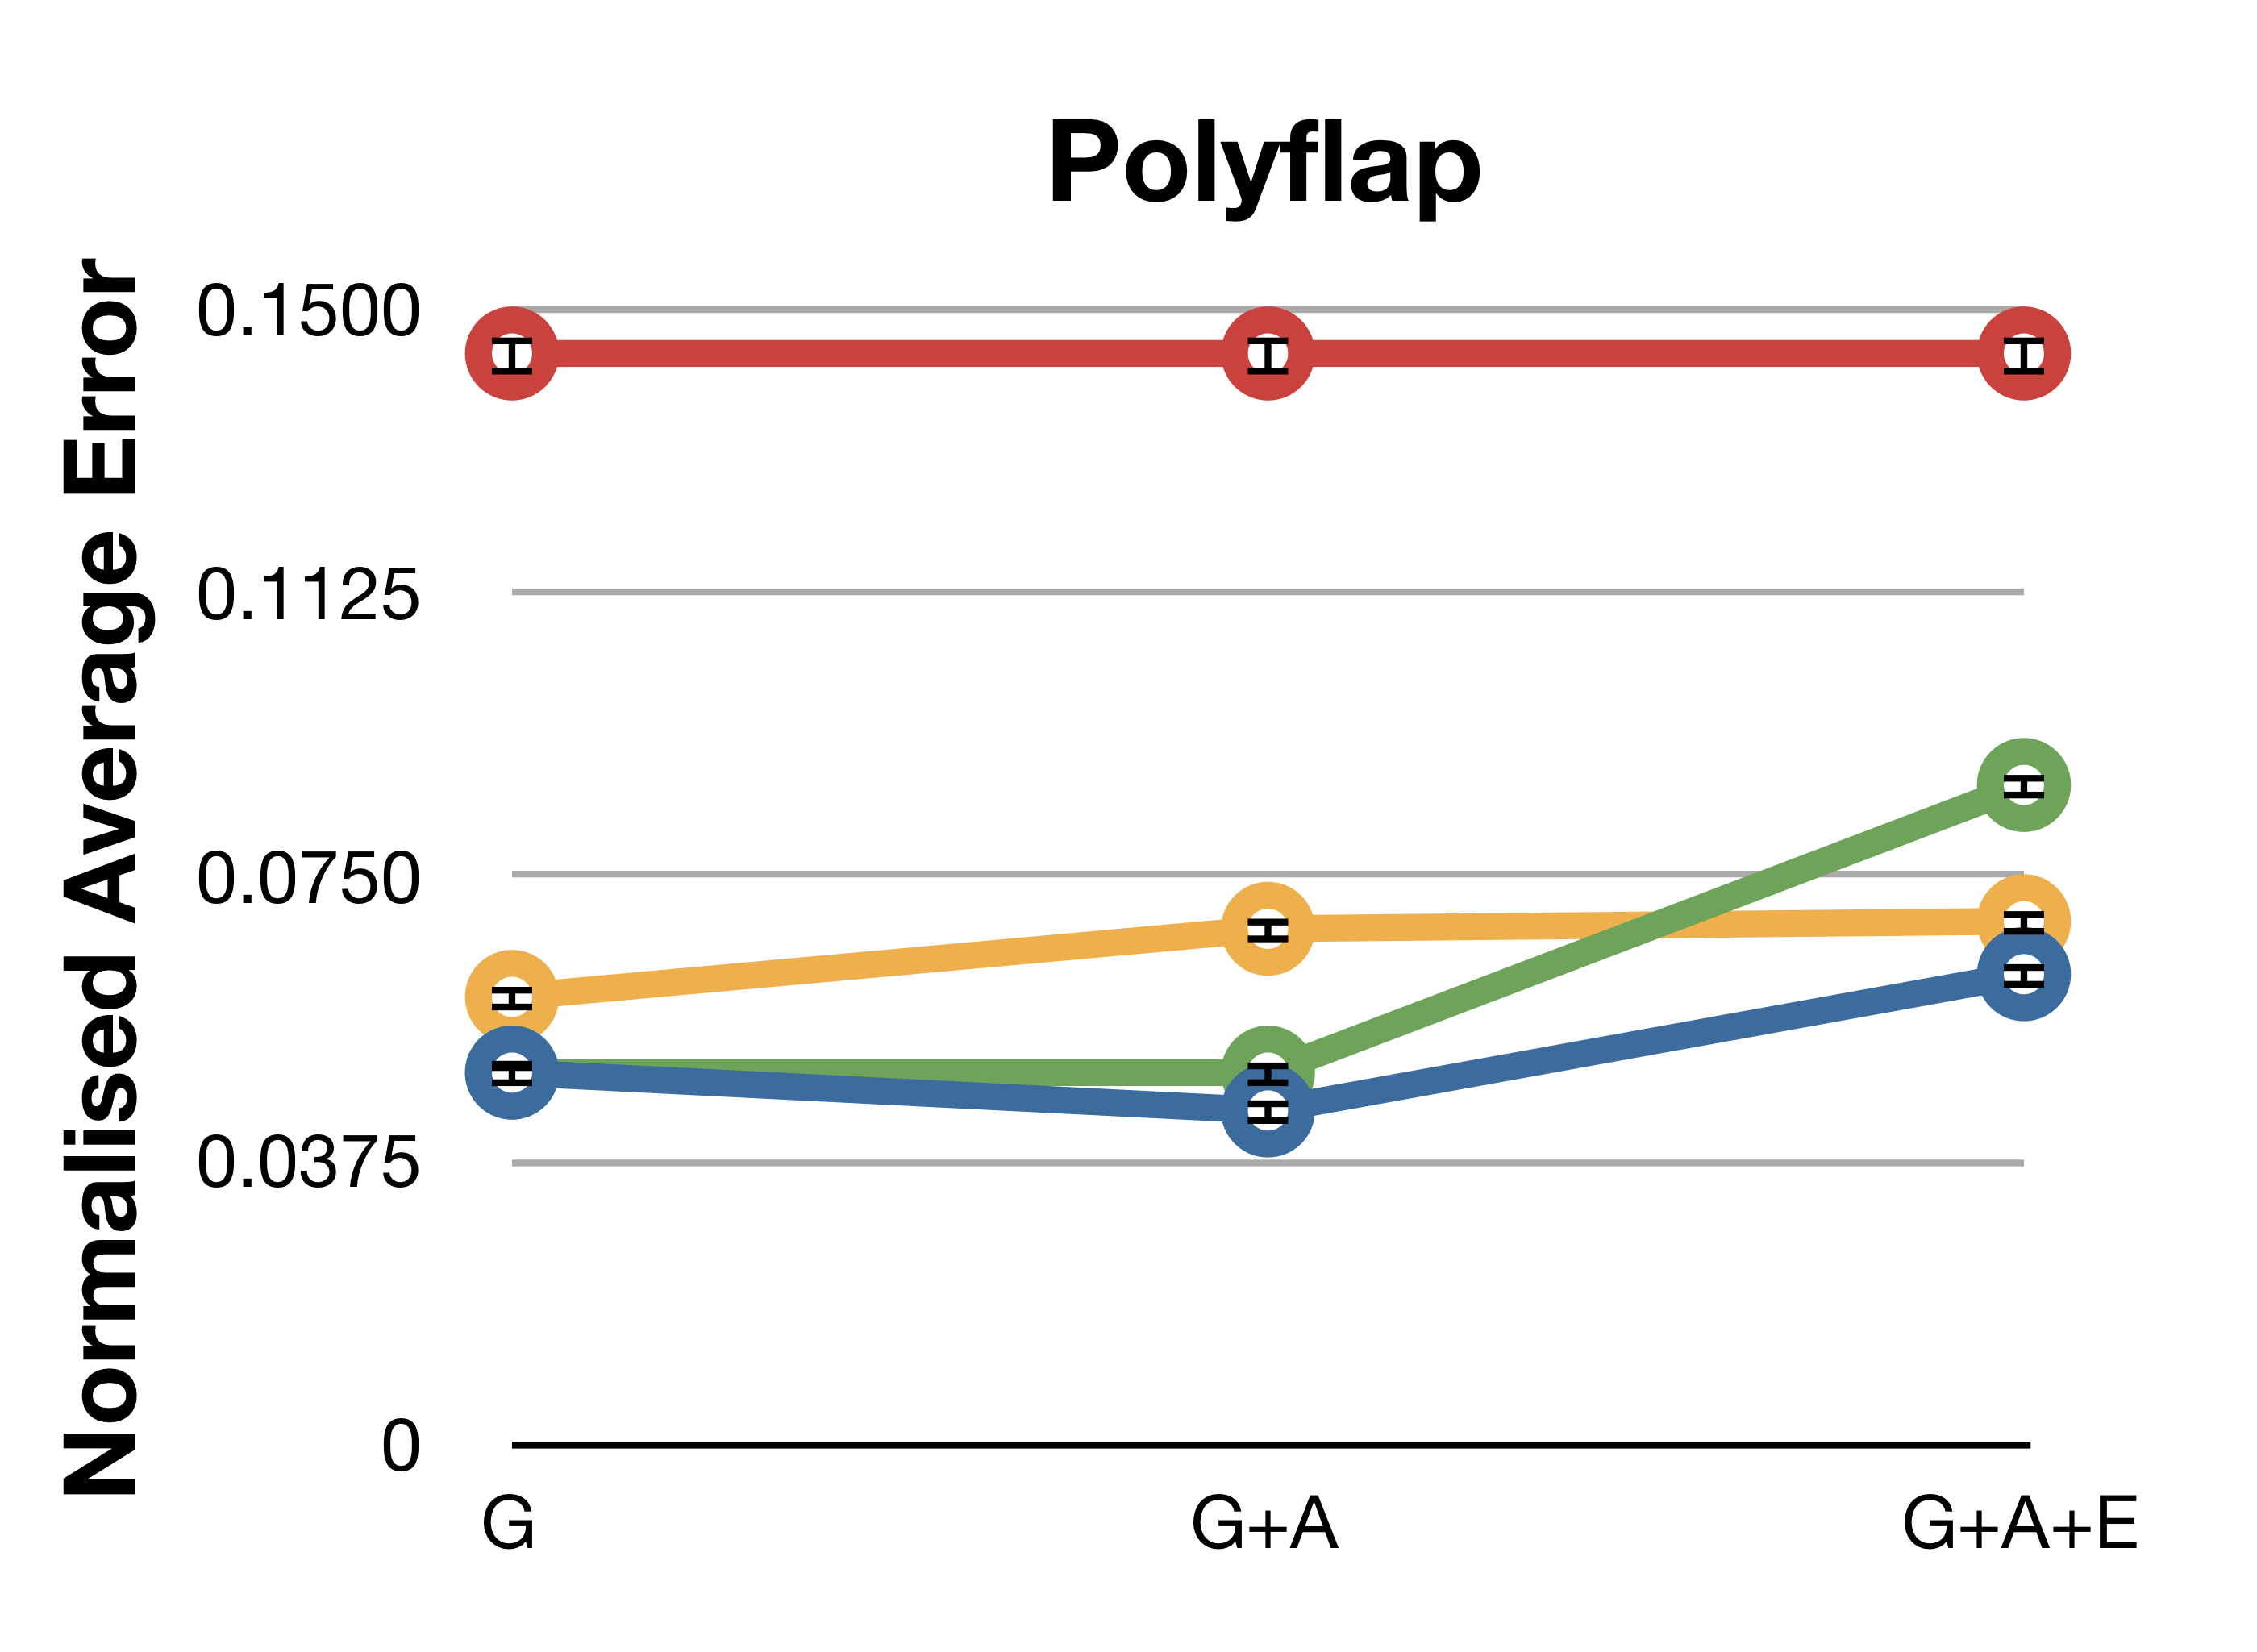
\includegraphics[width=0.45\columnwidth]{./L1av_graph_polyflap}
%}
%\centerline{
%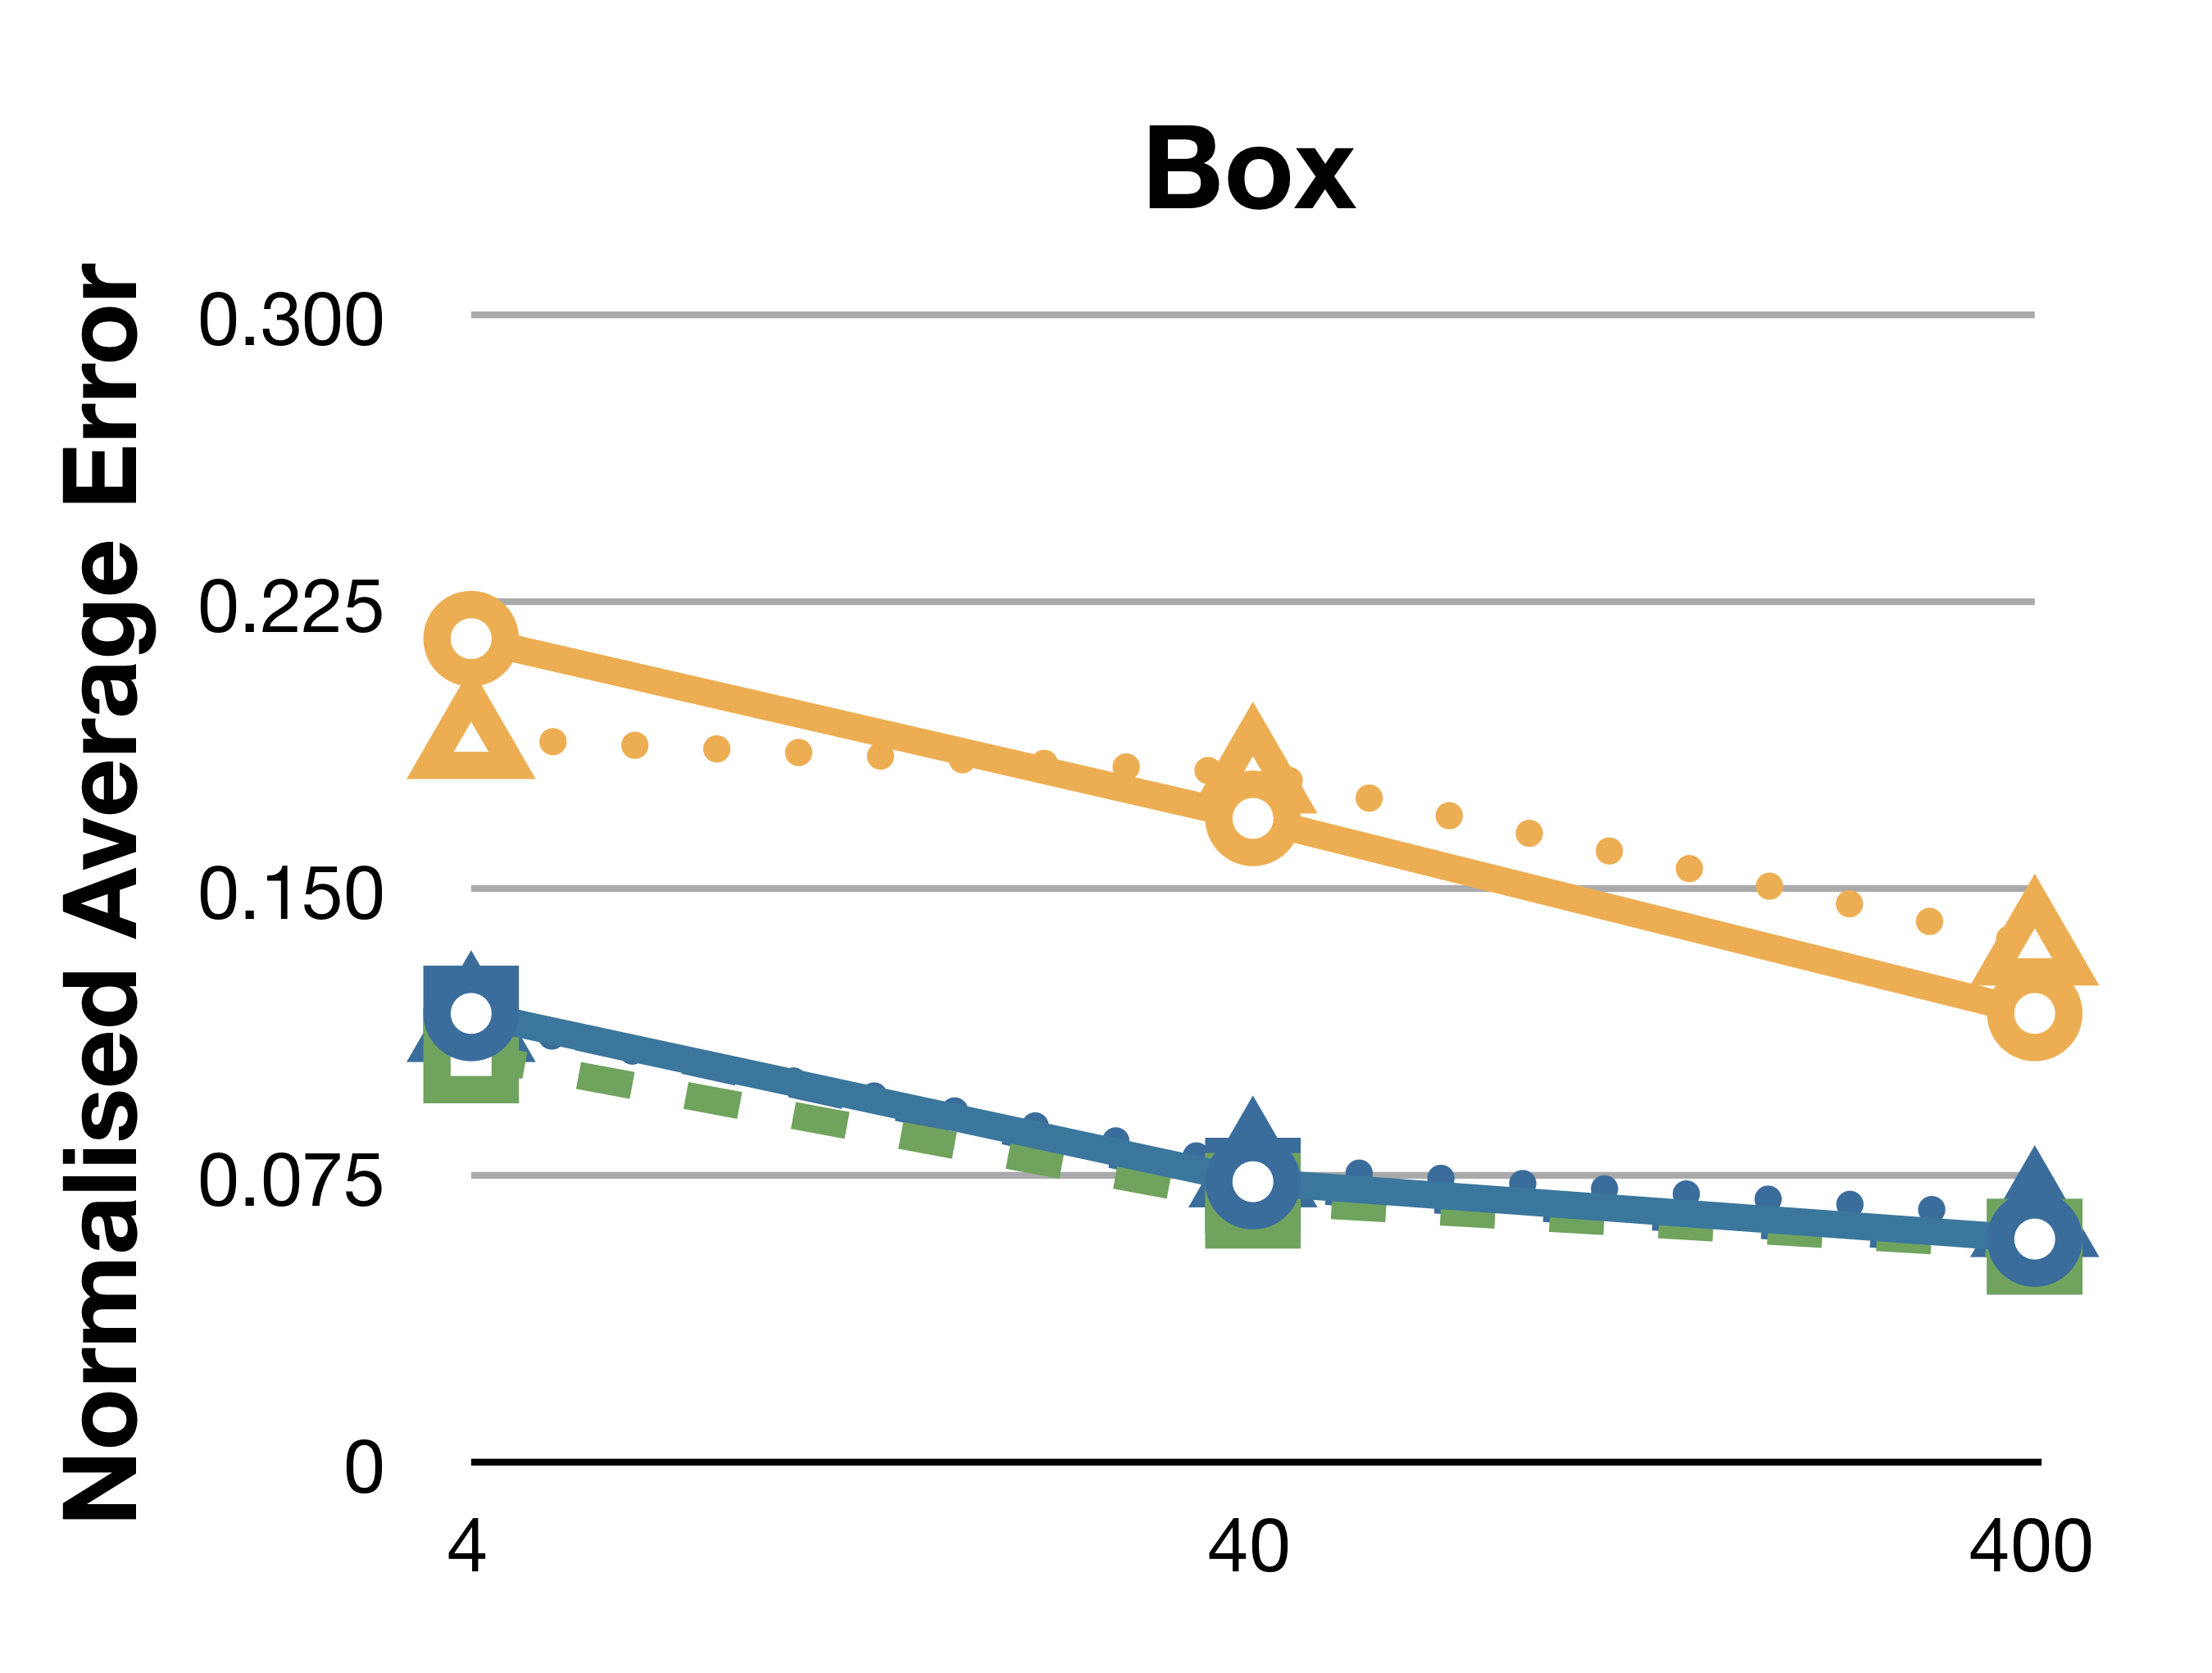
\includegraphics[width=0.45\columnwidth]{./L2av_graph}
%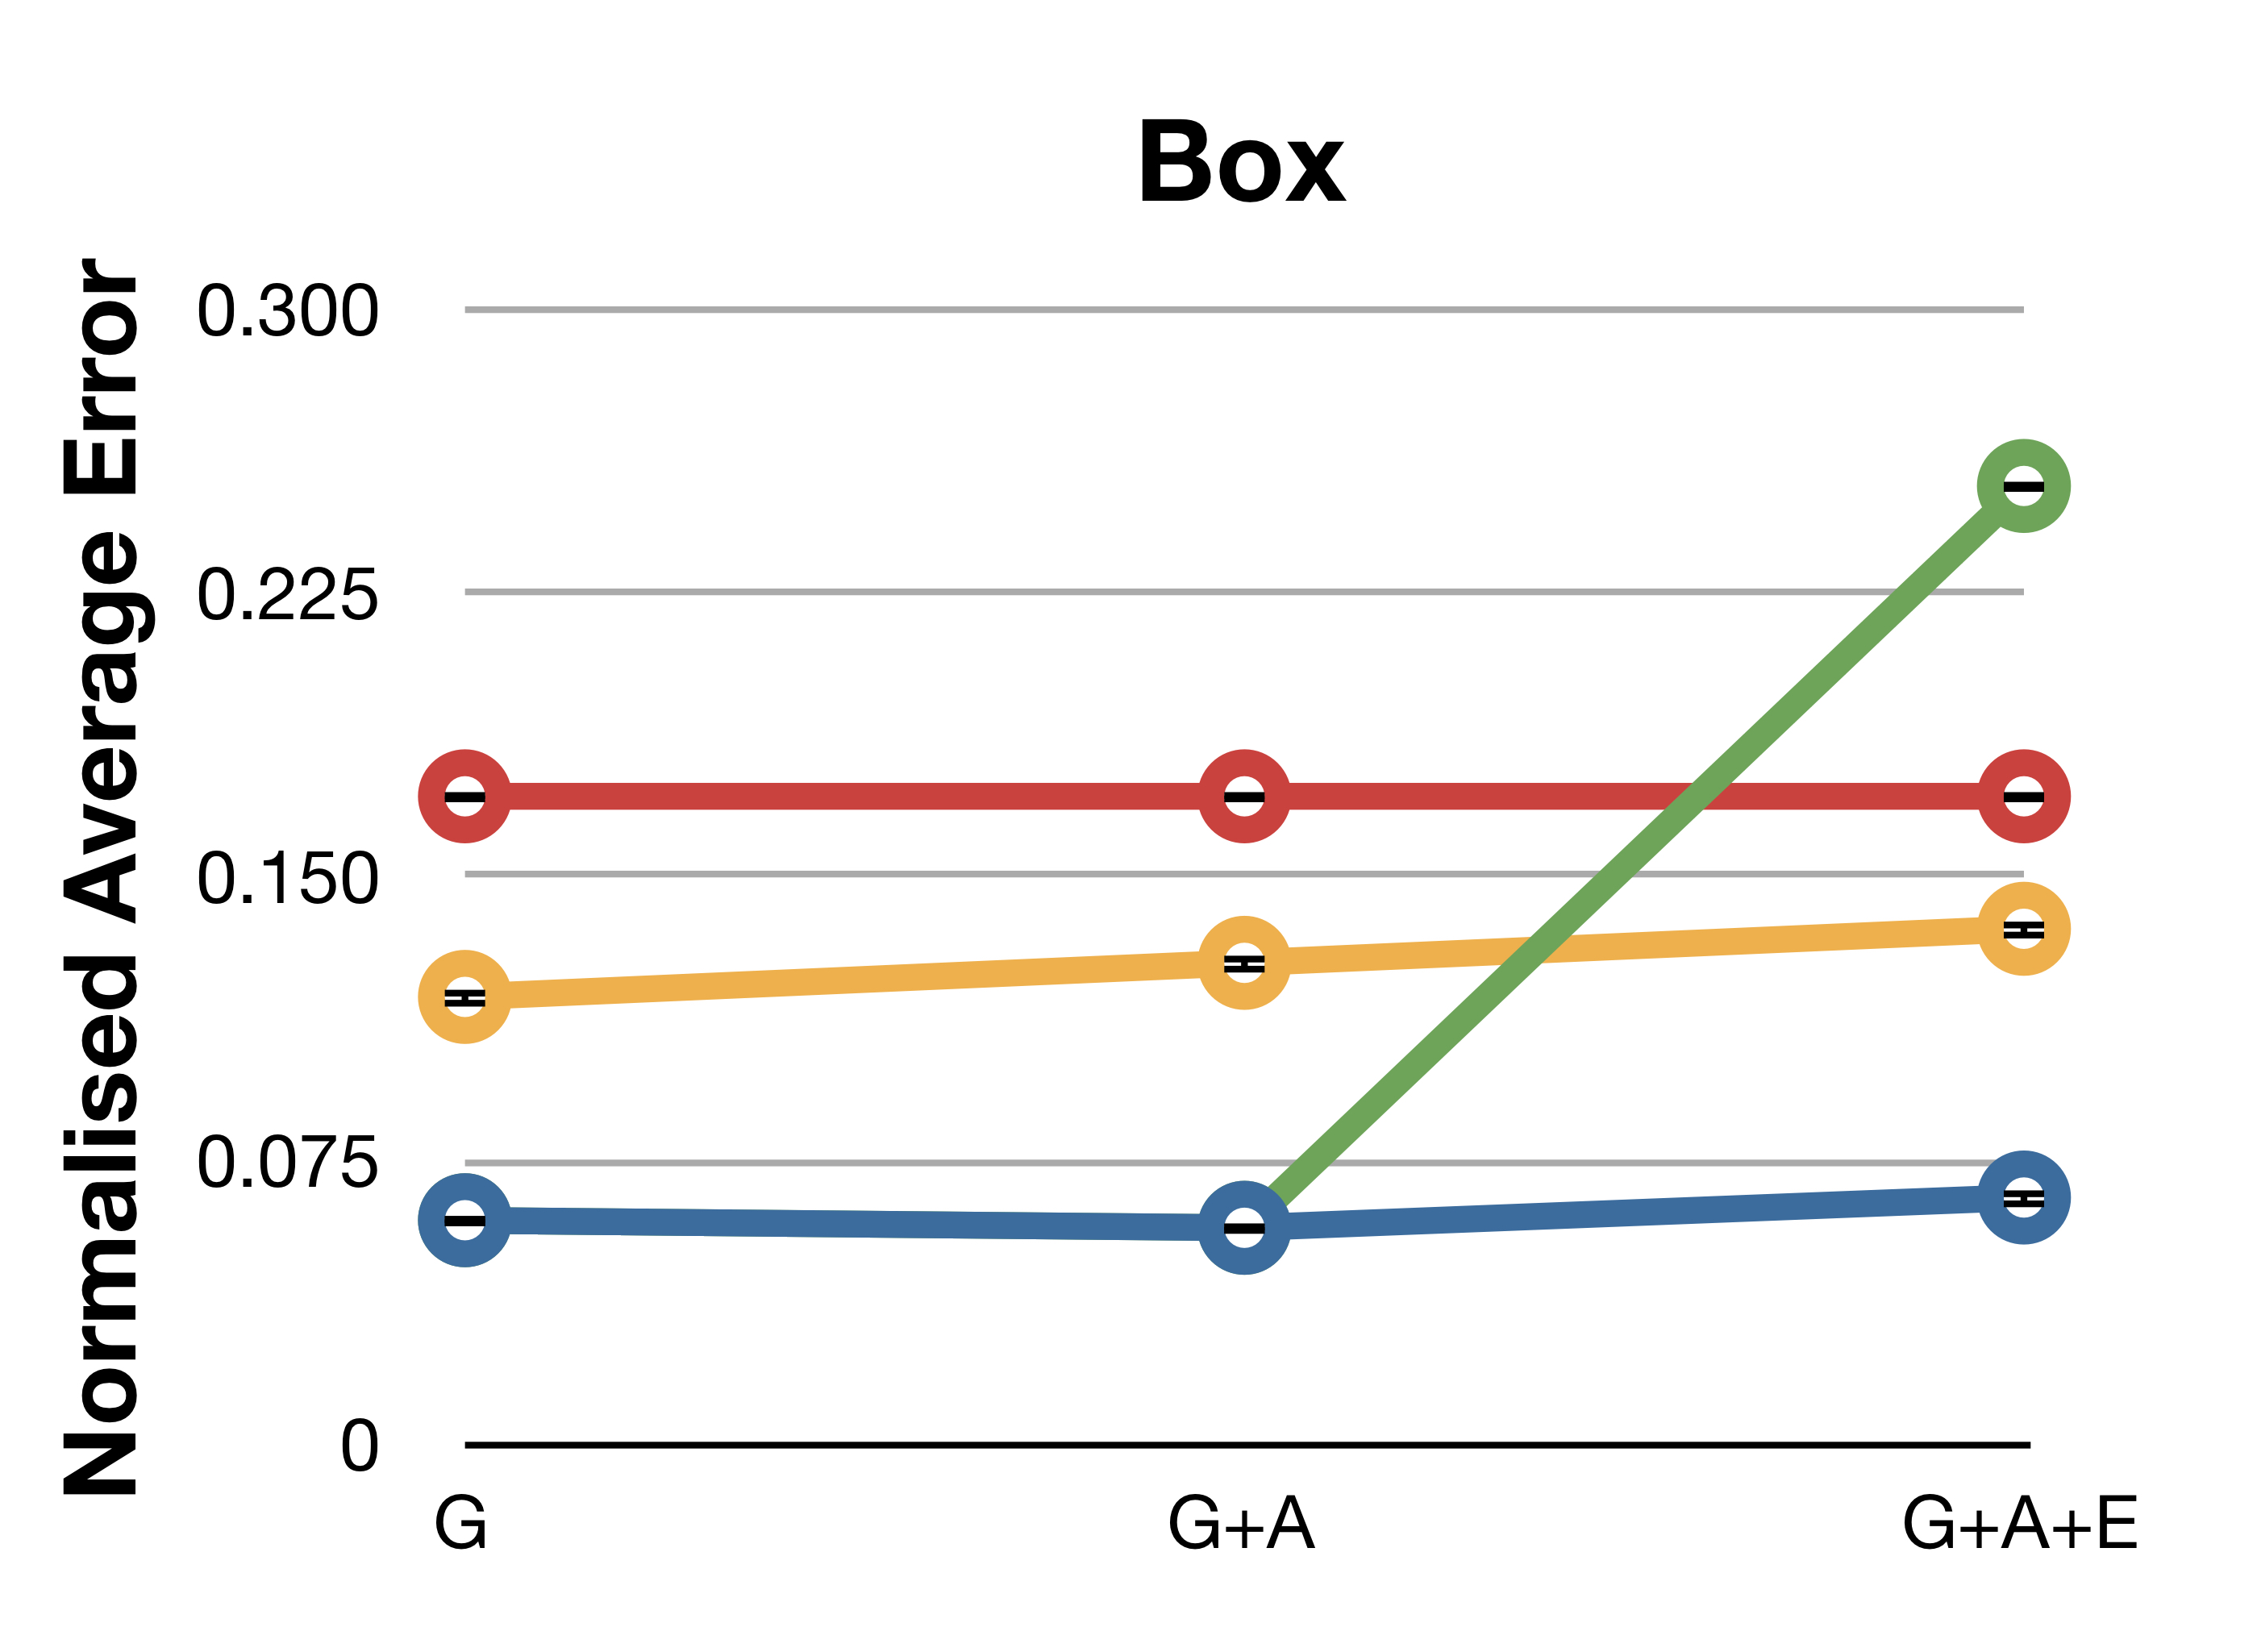
\includegraphics[width=0.45\columnwidth]{./L1av_graph_box}
%}
%\centerline{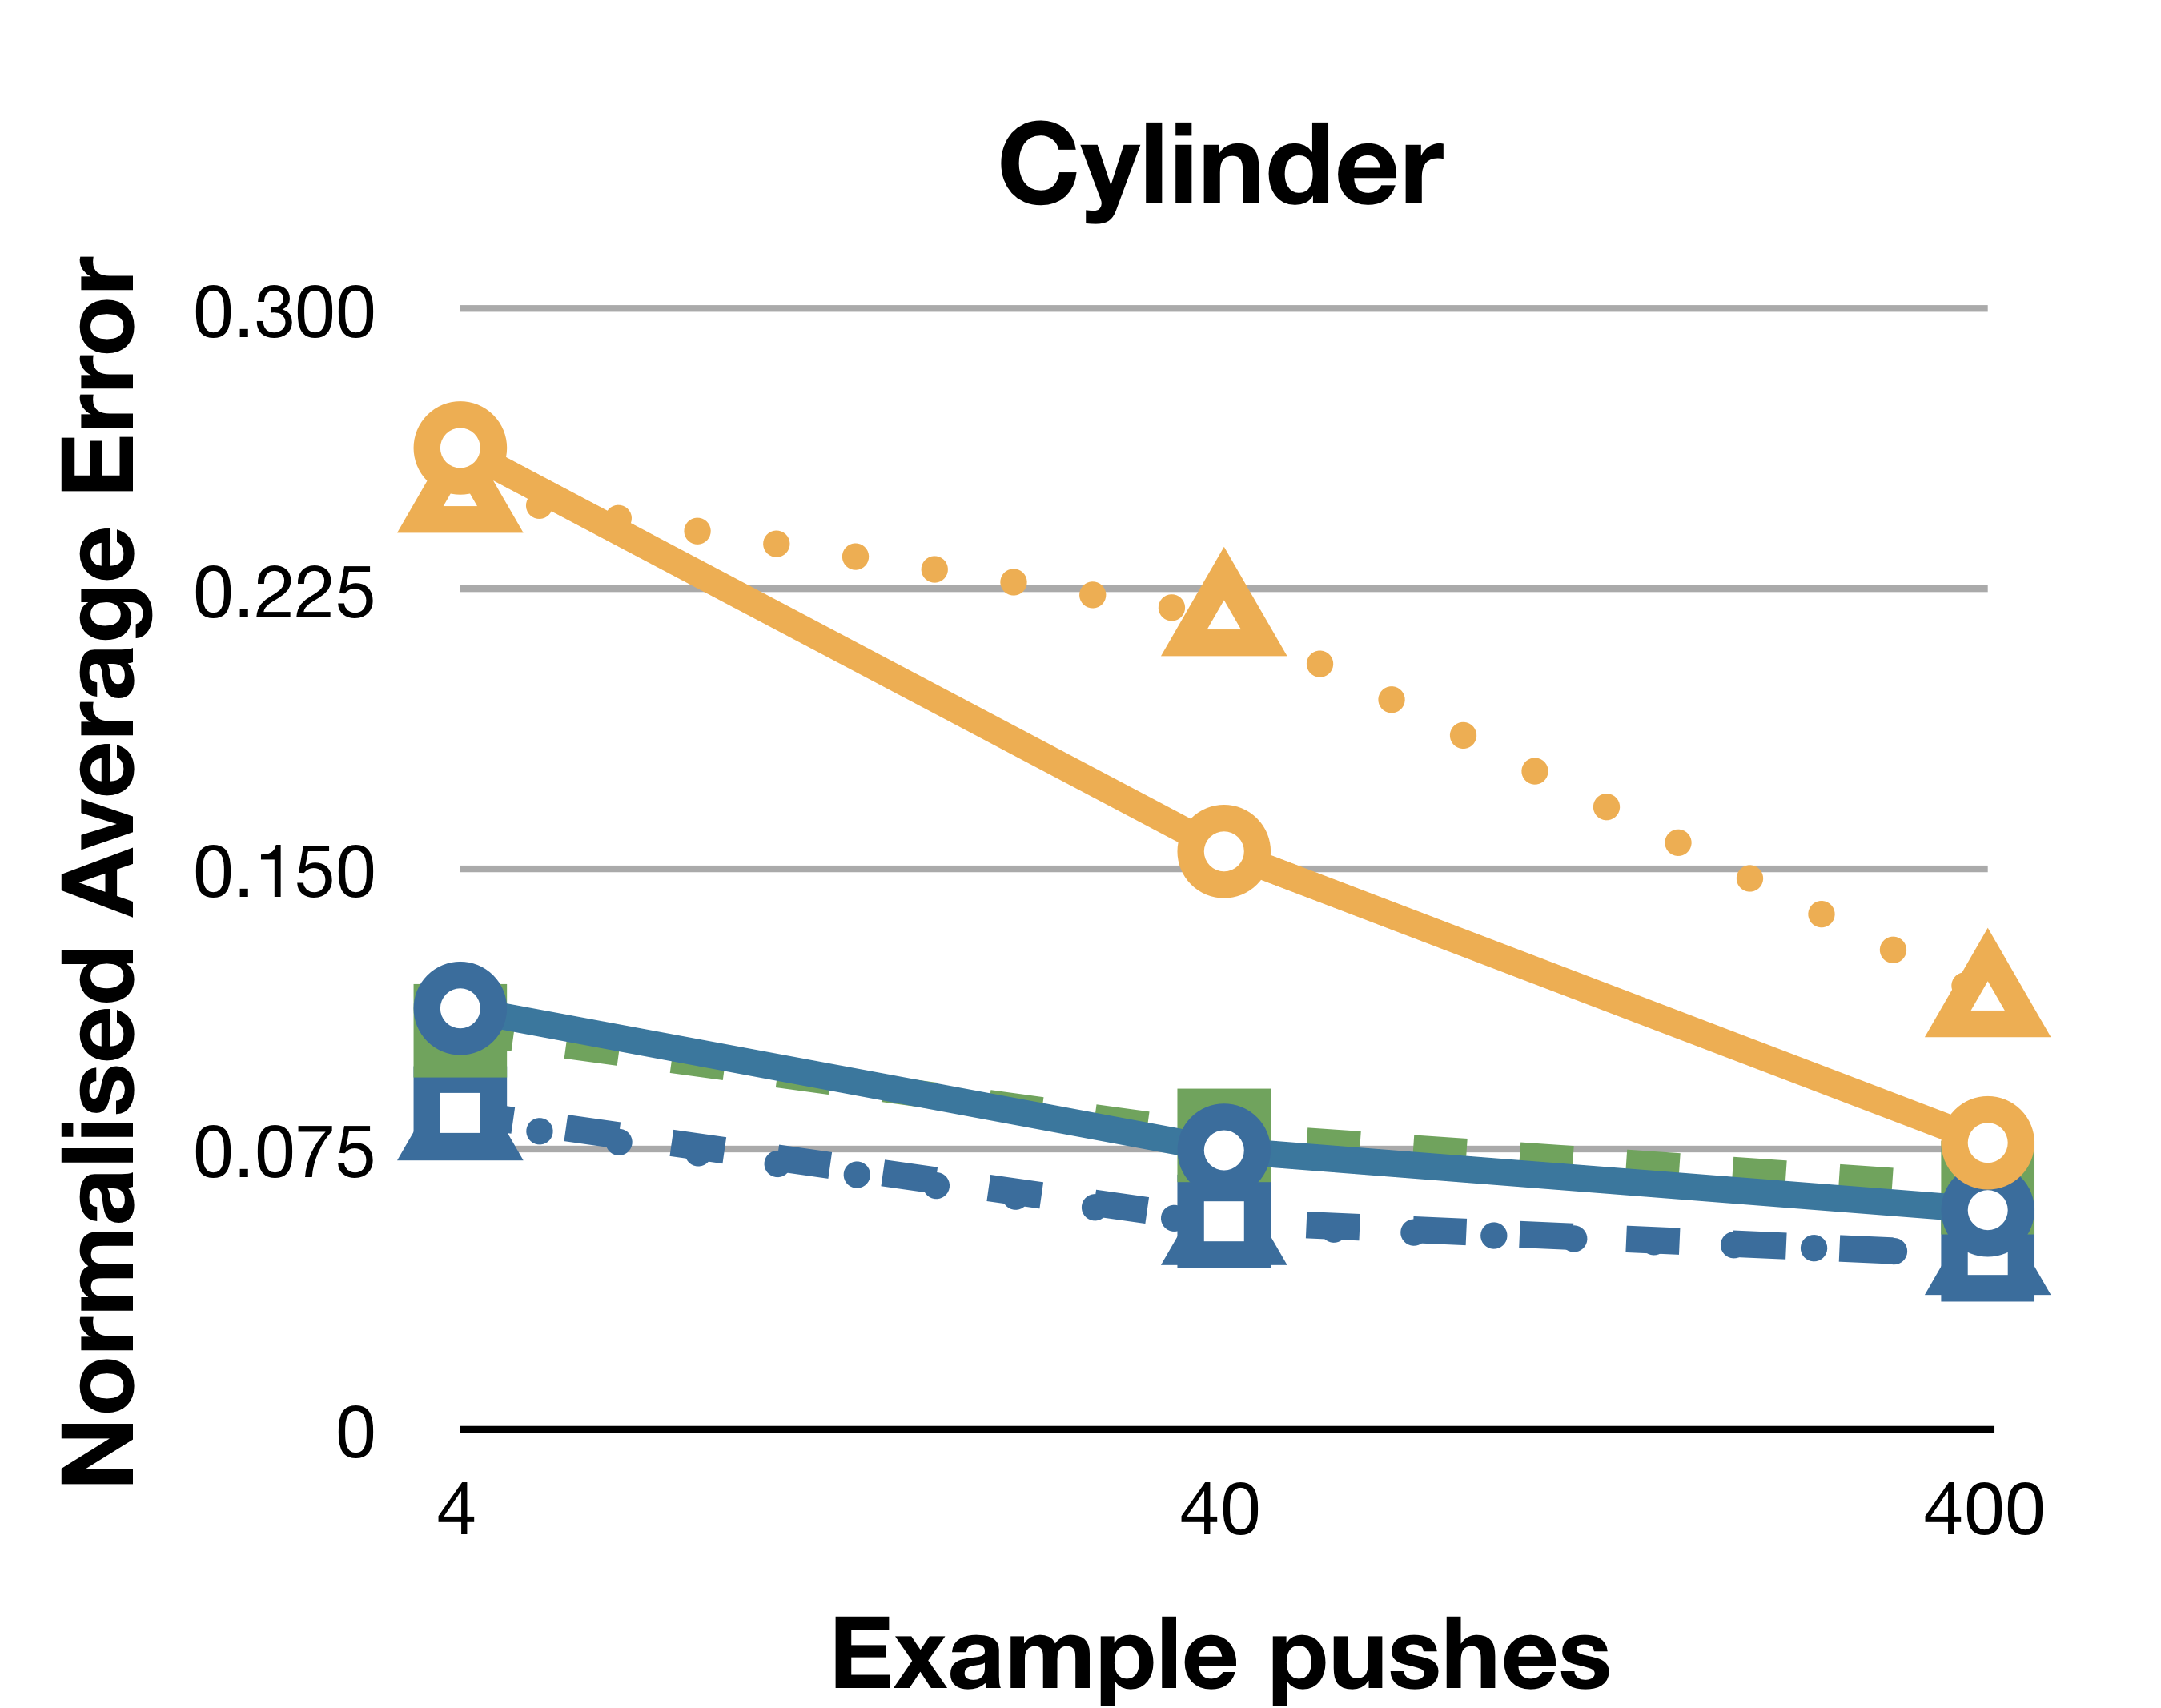
\includegraphics[width=0.45\columnwidth]{./L3av_graph}
%                 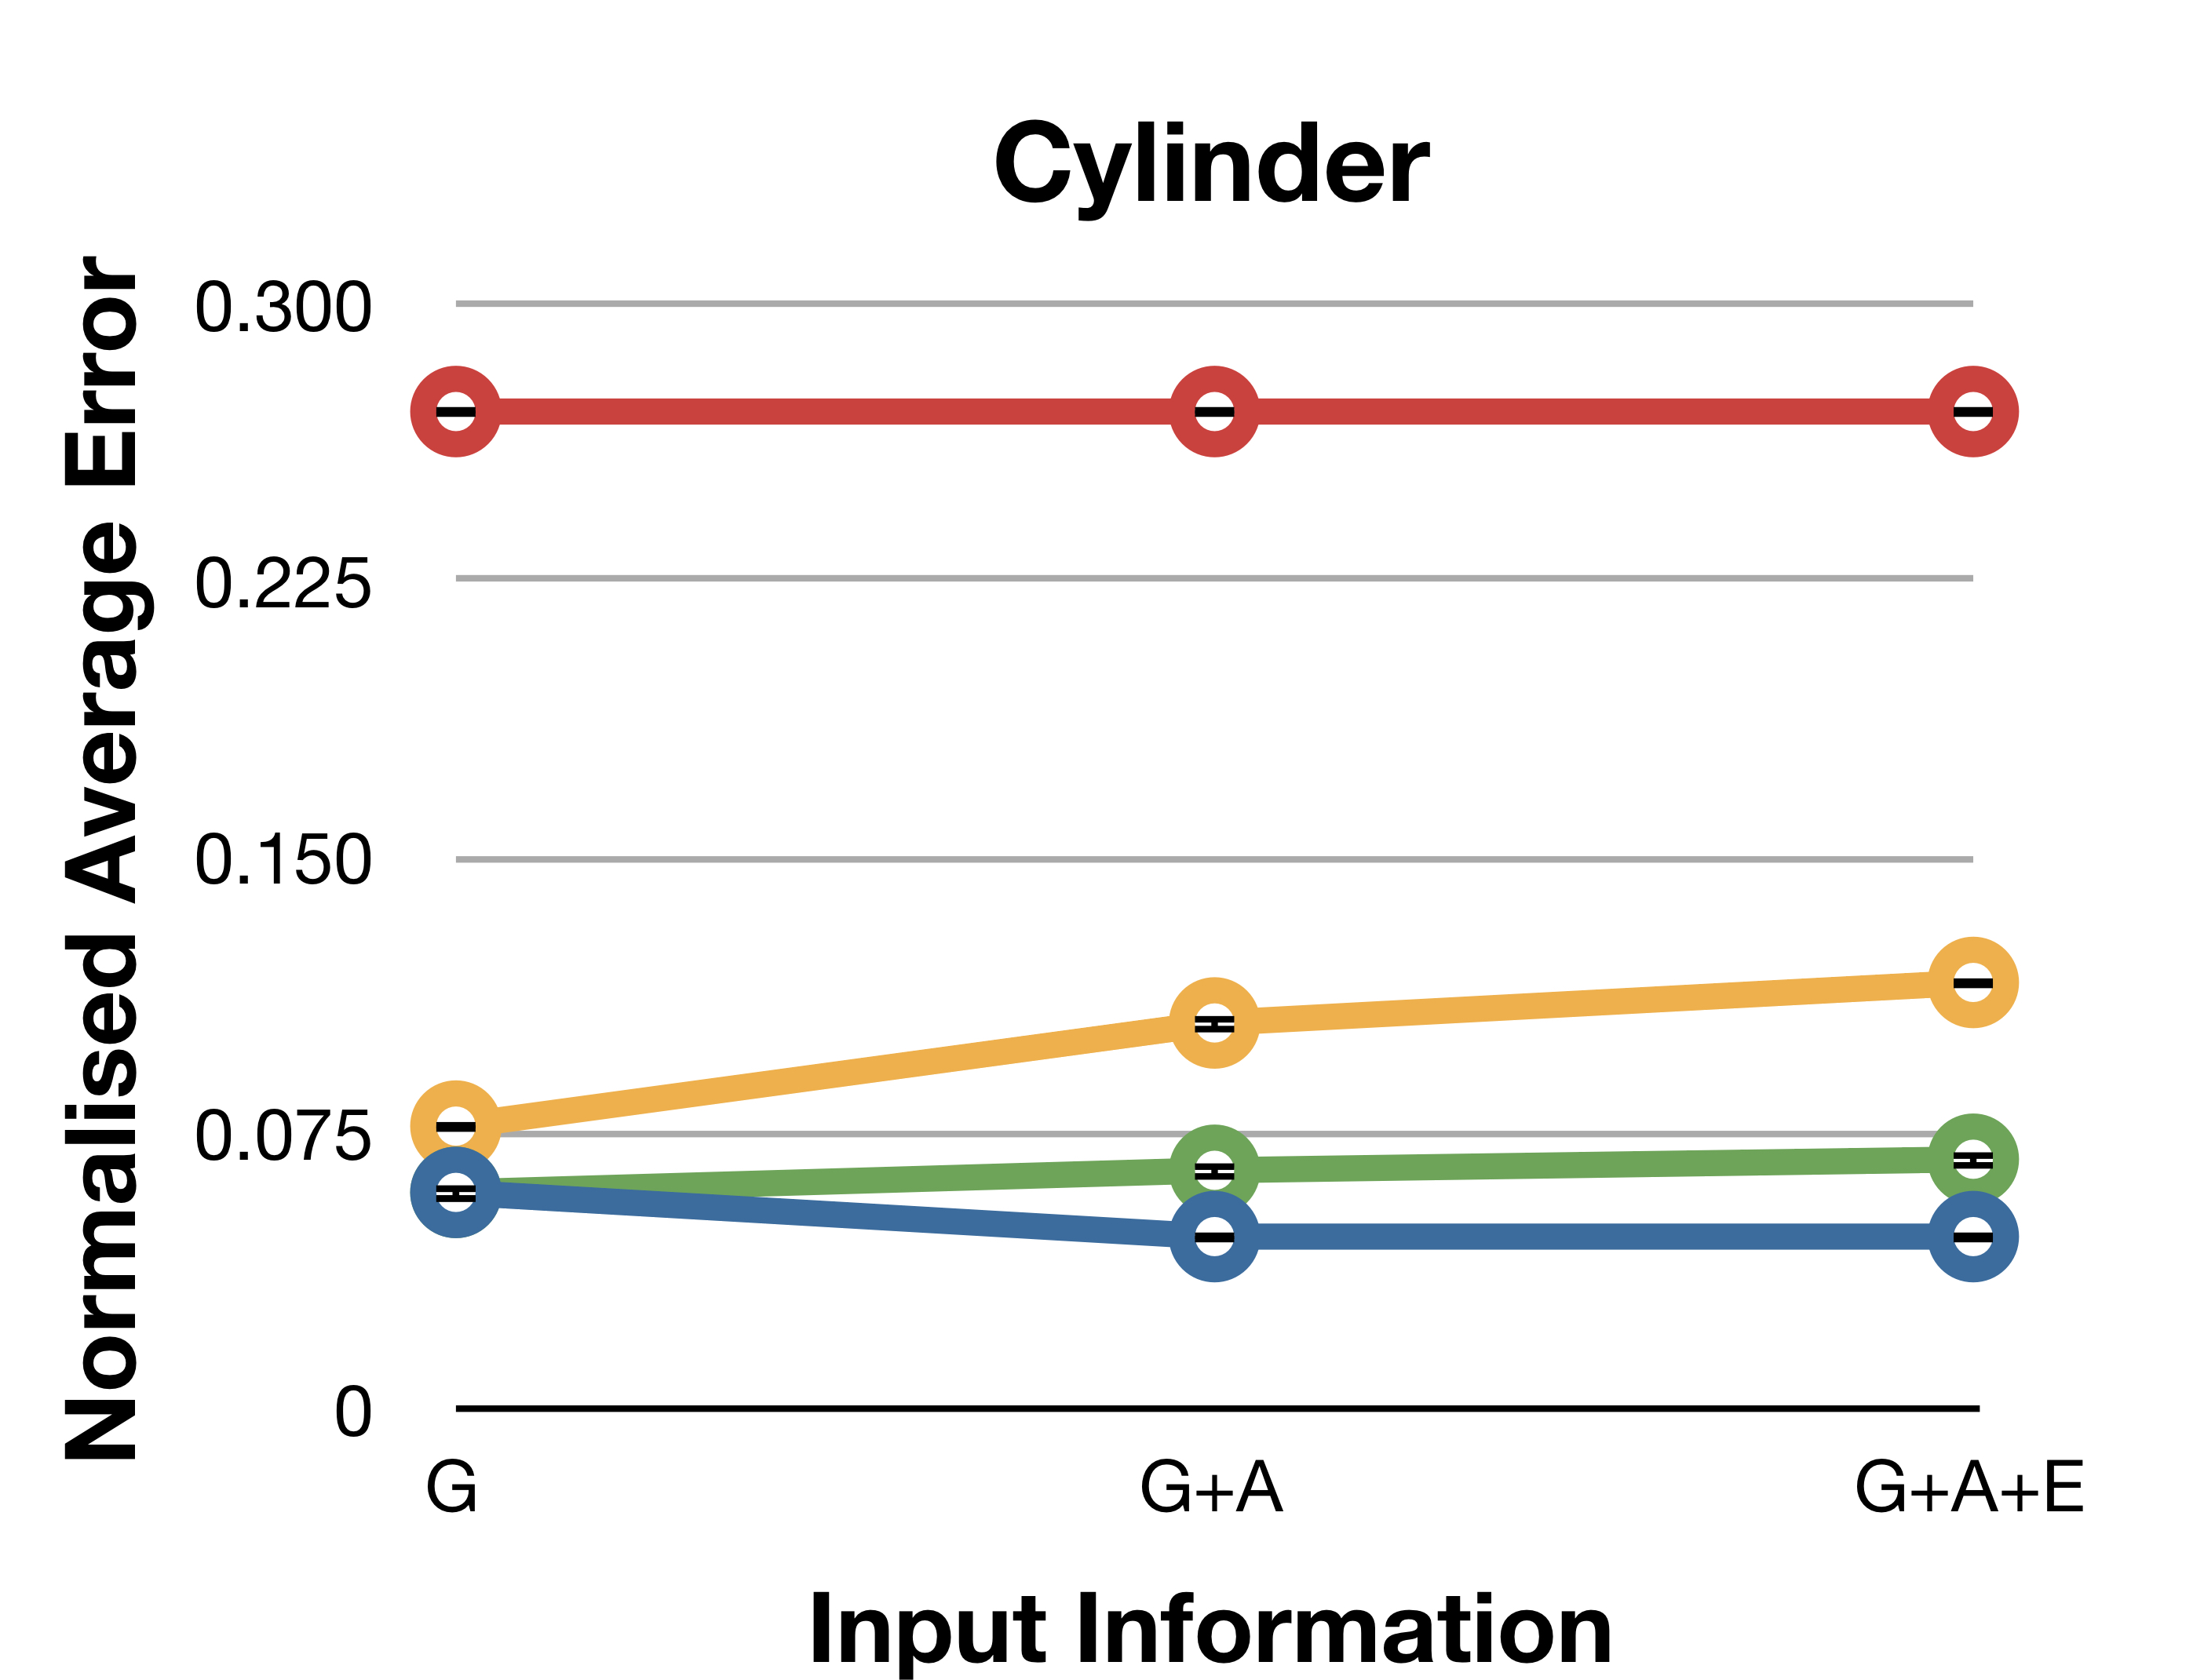
\includegraphics[width=0.45\columnwidth]{./L1av_graph_cylinder}
%}
%\centerline{
\includegraphics[width=\linewidth]{./L1_convergence_graph_key}
}
\vspace{-1mm}
\caption{Experiment P1: Convergence of learning for a cylinder on an uneven surface. \label{fig:Lgraph-uneven}}
\end{figure}

\newlength{\imgwid}
\setlength{\imgwid}{2.5cm}

\begin{figure}[htbp]
\centerline{
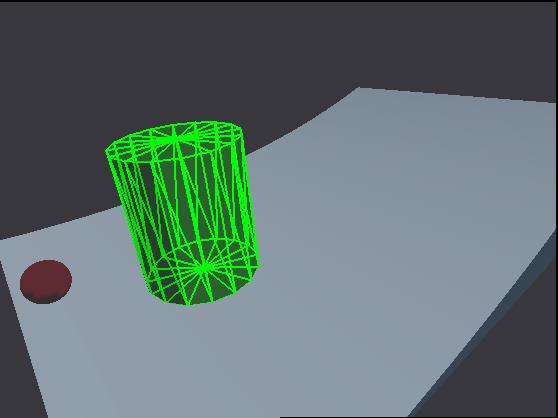
\includegraphics[width=\imgwid]{./A00000}
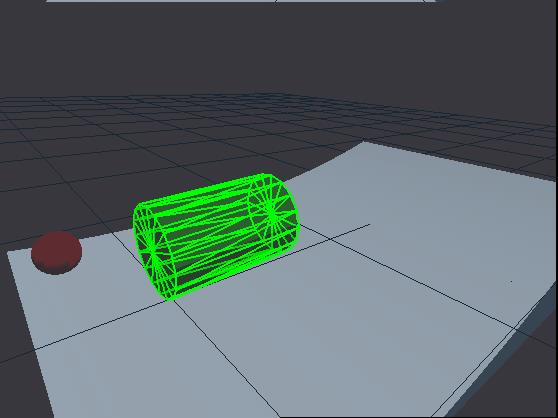
\includegraphics[width=\imgwid]{./B00257}
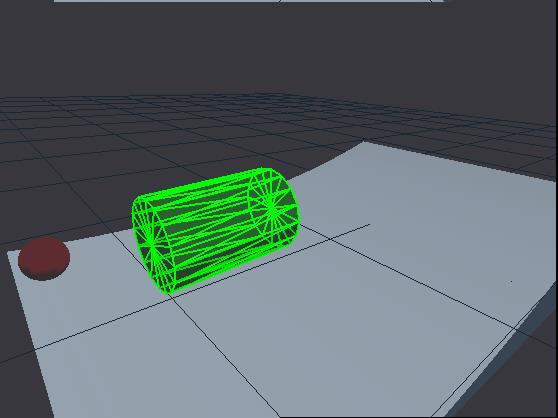
\includegraphics[width=\imgwid]{./C00900}
}
\centerline{
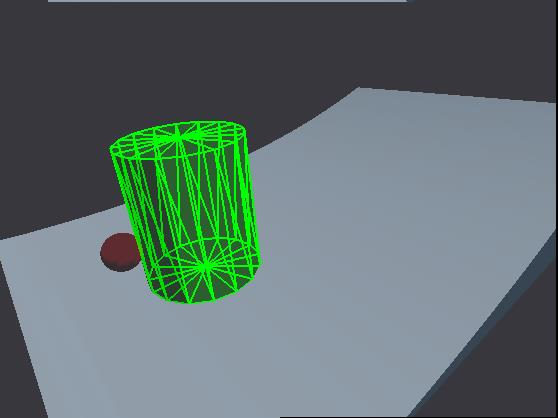
\includegraphics[width=\imgwid]{./A00050}
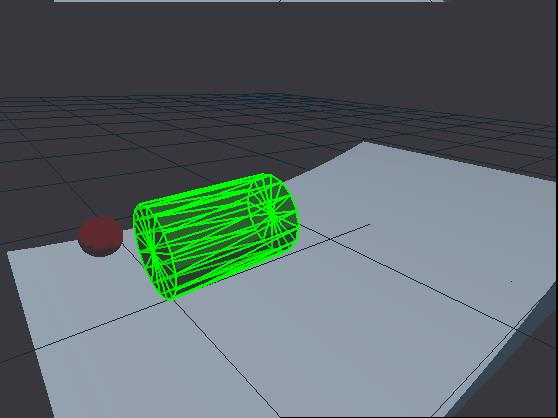
\includegraphics[width=\imgwid]{./B00300}
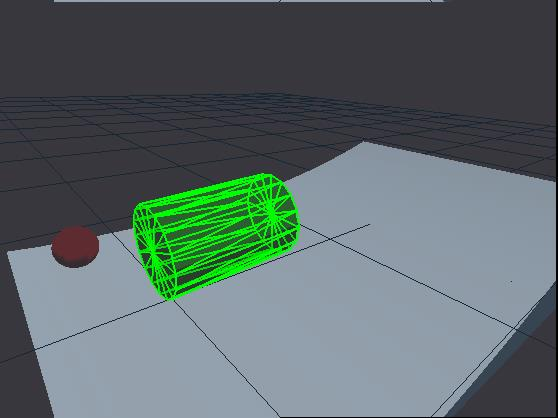
\includegraphics[width=\imgwid]{./C00950}
}
\centerline{
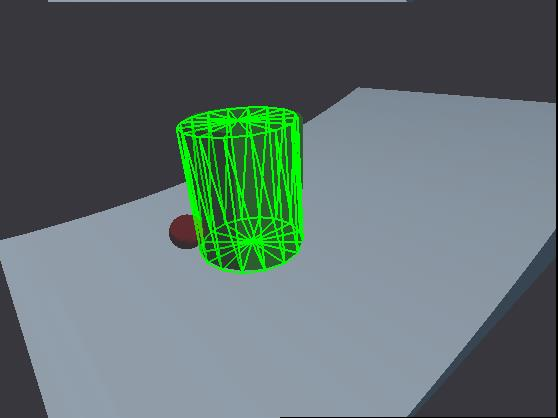
\includegraphics[width=\imgwid]{./A00100}
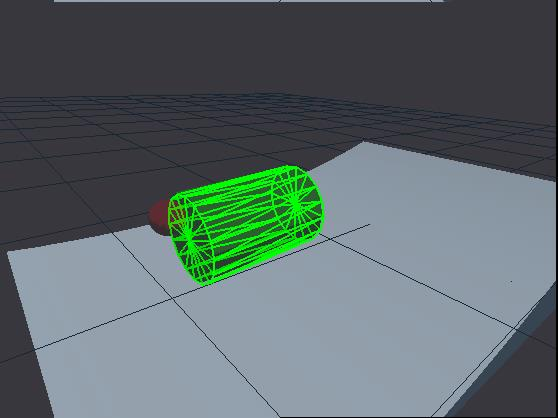
\includegraphics[width=\imgwid]{./B00350}
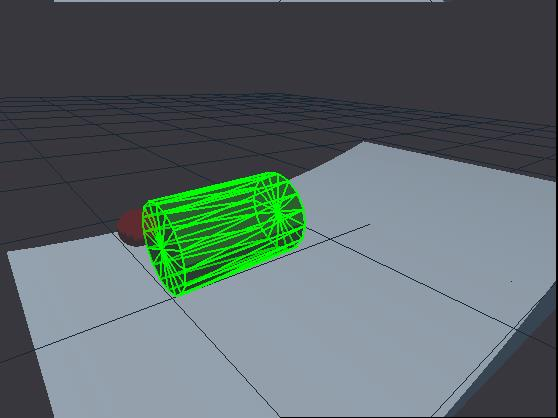
\includegraphics[width=\imgwid]{./C01000}
}
\centerline{
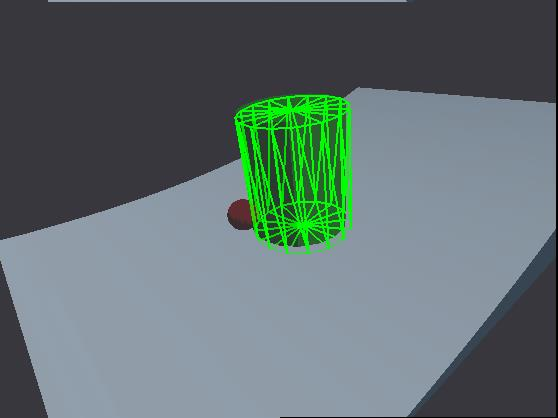
\includegraphics[width=\imgwid]{./A00150}
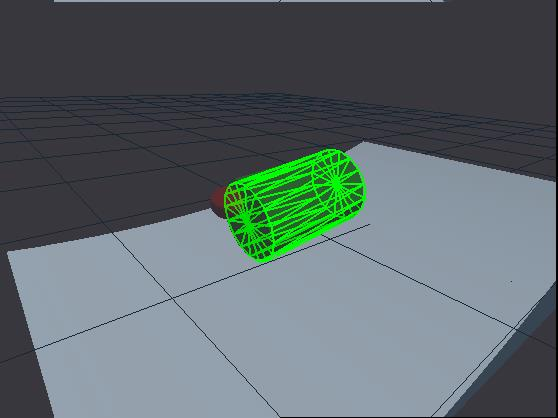
\includegraphics[width=\imgwid]{./B00400}
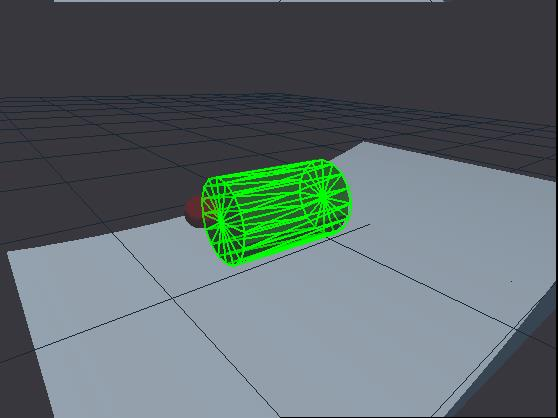
\includegraphics[width=\imgwid]{./C01050}
}
%\vspace{0.1cm}
\centerline{
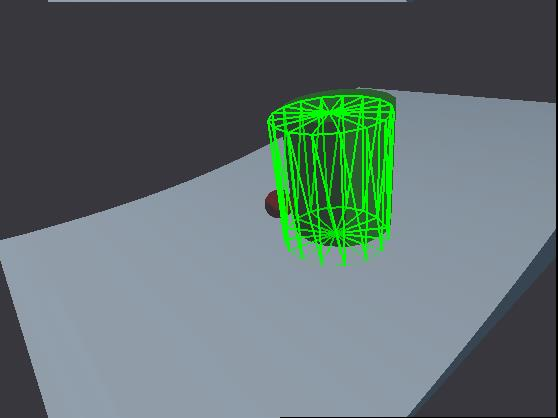
\includegraphics[width=\imgwid]{./A00200}
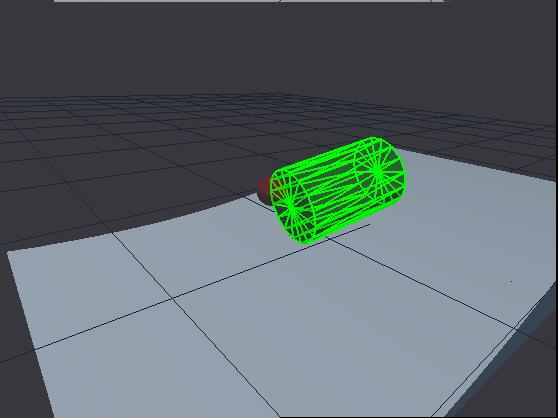
\includegraphics[width=\imgwid]{./B00450}
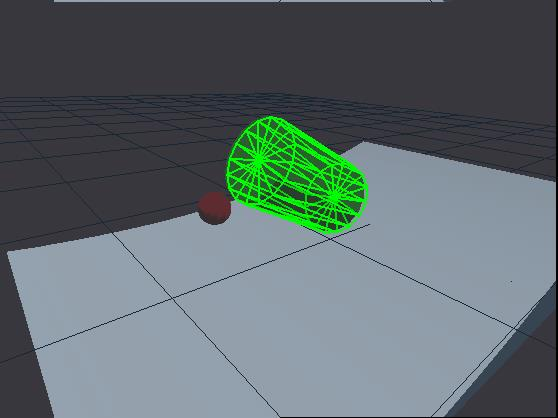
\includegraphics[width=\imgwid]{./C01063}
}
%\vspace{0.1cm}
\centerline{
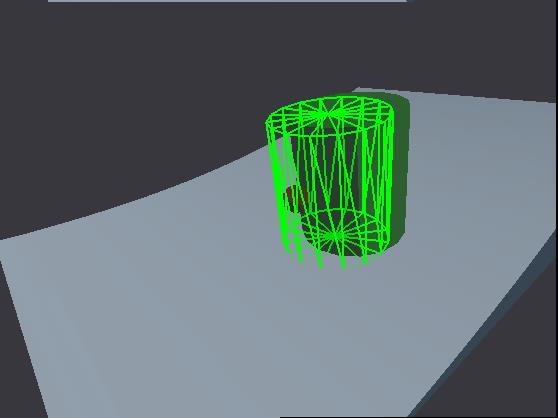
\includegraphics[width=\imgwid]{./A00250}
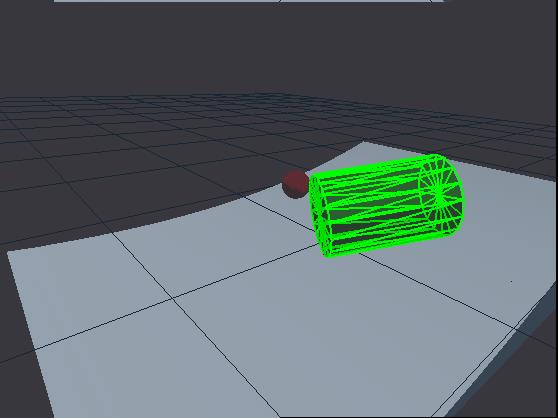
\includegraphics[width=\imgwid]{./B00500}
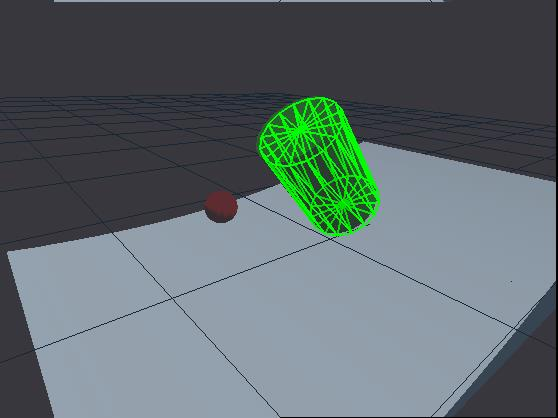
\includegraphics[width=\imgwid]{./C01069}
}
\centerline{
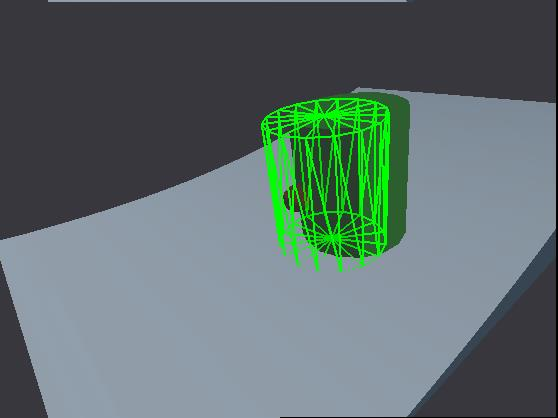
\includegraphics[width=\imgwid]{./A00295}
\includegraphics[width=\imgwid]{./B00550}
\includegraphics[width=\imgwid]{./C01100}
}
\caption {Experiment P1: predictions for a simulated cylinder on a non-planar surface. Predictions were made over 150 steps by the KDEF-GA/quat method. Note that the learned model can correctly predict for two starting orientations, and for dynamic flipping and rolling motions once the finger loses contact.
\label{fig:ExperimentL1-uneven}}
\end{figure}

\begin{table*}[t]
\begin{center}
\begin{tabular}{|l|l|l|l|l|}
\cline{1-4}
Predictor & Polyflap & Box & Cylinder \\
\cline{1-4}
KDEF-Ge & 0.055$\pm$0.002 & 0.061$\pm$0.003 & 0.063$\pm$0.003\\
KDEF-Gq  & \textbf{0.049}$\pm$0.002 & \textbf{0.059}$\pm$0.002 & \textbf{0.059}$\pm$0.003\\
KDEF-Gv   & 0.057$\pm$0.002 & 0.066$\pm$0.003 & 0.071$\pm$0.003\\
LWPR-Ge &  0.059$\pm$0.002 & 0.118$\pm$0.003 & 0.077$\pm$0.003\\
\cline{1-4}
KDEF-GAe & 0.054$\pm$0.002 & 0.060$\pm$0.003 & 0.052$\pm$0.002\\
KDEF-GAq & \textbf{0.044}$\pm$0.002 & \textbf{0.057}$\pm$0.002 & \textbf{0.047}$\pm$0.002\\
KDEF-GAv  & 0.064$\pm$0.002 & 0.097$\pm$0.002  & 0.109$\pm$0.003 \\
LWPR-GAe & 0.068$\pm$0.002 & 0.127$\pm$0.003 & 0.105$\pm$0.002 \\
\cline{1-4}
KDEF-GAEe & 0.083$\pm$0.003 & 0.065$\pm$0.003 & 0.050$\pm$0.002 \\
KDEF-GAEq & \textbf{0.062}$\pm$0.002 & \textbf{0.065}$\pm$0.003 & \textbf{0.047}$\pm$0.002\\
KDEF-GAEv & 0.081$\pm$0.002 & 0.086$\pm$0.002 & 0.065$\pm$0.002\\
LWPR-GAEe & 0.069$\pm$0.002 & 0.136$\pm$0.003 & 0.116$\pm$0.003\\
\cline{1-4}
KDE-GAe & 0.053$\pm$0.002 & 0.057$\pm$0.002 & 0.068$\pm$0.003 \\
KDE-GAq  & \textbf{0.049}$\pm$0.002 & \textbf{0.057}$\pm$0.002 & \textbf{0.065}$\pm$0.003\\
KDE-GAv   & 0.062$\pm$0.002 & 0.058$\pm$0.002 & 0.092$\pm$0.004\\
\cline{1-4}
KDE-GAEe & 0.090$\pm$0.002 & 0.161$\pm$0.003 & 0.071$\pm$0.003\\
KDE-GAEq  & \textbf{0.087}$\pm$0.002 & 0.253$\pm$0.002 & \textbf{0.068}$\pm$0.003\\
KDE-GAEv   & \textbf{0.087}$\pm$0.002 & \textbf{0.127}$\pm$0.003 & 0.091$\pm$0.004\\
\cline{1-4}
PhysX & 0.144$\pm$0.003 &  0.171$\pm$0.003 & 0.271$\pm$0.001\\
\cline{1-4}
\end{tabular}
\caption[Performance Table]{Experiment P1: Forward push on a
  polyflap/box/cylinder, trained on real data. Shown is the dimensionless measure normalised average error  ${E_{av}^{norm}} \pm$ standard error. The parameterisations are denoted by e (Euler), q (Gauss Quaternion) and v (Gauss+Von-Mises Fisher) respectively. \label{tab:PerformanceTableL1av}
}
\end{center}
\end{table*}  

\newlength{\imgAXwid}
\setlength{\imgAXwid}{2.07cm}

\begin{figure*}[htbp]
\centerline{
\includegraphics[width=\imgAXwid]{./A1_2exp_667_1}
\includegraphics[width=\imgAXwid]{./A1_2exp_876_1}
\includegraphics[width=\imgAXwid]{./A2_2exp_399_1}
\includegraphics[width=\imgAXwid]{./A2_LWPR1_399_1}
\includegraphics[width=\imgAXwid]{./A2_2exp_87_1}
\includegraphics[width=\imgAXwid]{./A3_2exp_39_1}
\includegraphics[width=\imgAXwid]{./A3_LWPR1_39_1}
\includegraphics[width=\imgAXwid]{./A3_physx_39_1}
}
\centerline{
\includegraphics[width=\imgAXwid]{./A1_2exp_667_2}
\includegraphics[width=\imgAXwid]{./A1_2exp_876_2}
\includegraphics[width=\imgAXwid]{./A2_2exp_399_2}
\includegraphics[width=\imgAXwid]{./A2_LWPR1_399_2}
\includegraphics[width=\imgAXwid]{./A2_2exp_87_2}
\includegraphics[width=\imgAXwid]{./A3_2exp_39_2}
\includegraphics[width=\imgAXwid]{./A3_LWPR1_39_2}
\includegraphics[width=\imgAXwid]{./A3_physx_39_2}
}
% problem with physx @@@
%\vspace{0.1cm}
%\centerline{
%\includegraphics[width=\imgAXwid]{./A2_physx_399_1}
%\includegraphics[width=\imgAXwid]{./A2_physx_399_2}
%\includegraphics[width=\imgAXwid]{./A2_physx_399_3}
%\includegraphics[width=\imgAXwid]{./A2_physx_399_4}
%\includegraphics[width=\imgAXwid]{./A2_physx_399_5}
%}
%\vspace{0.1cm}
\centerline{
\includegraphics[width=\imgAXwid]{./A1_2exp_667_3}
\includegraphics[width=\imgAXwid]{./A1_2exp_876_3}
\includegraphics[width=\imgAXwid]{./A2_2exp_399_3}
\includegraphics[width=\imgAXwid]{./A2_LWPR1_399_3}
\includegraphics[width=\imgAXwid]{./A2_2exp_87_3}
\includegraphics[width=\imgAXwid]{./A3_2exp_39_3}
\includegraphics[width=\imgAXwid]{./A3_LWPR1_39_3}
\includegraphics[width=\imgAXwid]{./A3_physx_39_3}
}
\centerline{
\includegraphics[width=\imgAXwid]{./A1_2exp_667_4}
\includegraphics[width=\imgAXwid]{./A1_2exp_876_4}
\includegraphics[width=\imgAXwid]{./A2_2exp_399_4}
\includegraphics[width=\imgAXwid]{./A2_LWPR1_399_4}
\includegraphics[width=\imgAXwid]{./A2_2exp_87_4}
\includegraphics[width=\imgAXwid]{./A3_2exp_39_4}
\includegraphics[width=\imgAXwid]{./A3_LWPR1_39_4}
\includegraphics[width=\imgAXwid]{./A3_physx_39_4}
}
%\vspace{0.1cm}
\centerline{
\includegraphics[width=\imgAXwid]{./A1_2exp_667_5}
\includegraphics[width=\imgAXwid]{./A1_2exp_876_5}
\includegraphics[width=\imgAXwid]{./A2_2exp_399_5}
\includegraphics[width=\imgAXwid]{./A2_LWPR1_399_5}
\includegraphics[width=\imgAXwid]{./A2_2exp_87_5}
\includegraphics[width=\imgAXwid]{./A3_2exp_39_5}
\includegraphics[width=\imgAXwid]{./A3_LWPR1_39_5}
\includegraphics[width=\imgAXwid]{./A3_physx_39_5}
}
%\vspace{0.1cm}
\caption {Experiment P1: polyflap, box and cylinder. Green outline shows
  predictions. Columns 1-2: KDEF-GA/quat on two trials exhibiting
  different motions of the polyflap. Col 3: KDEF-GA/quat. Col 4: LWPR-G for one trial in
  which the box topples over. Col 5: KDEF-GA/quat on another trial in
  which the box slides. Columns 6-8 show the same push of the
  cylinder. Col 6: KDEF-GA/quat. Col 7: LWPR-G. Col 8: PhysX. Note tha
  for columns 6-7 the orientation of the cylinder is show by the
  rotating frame. Only the learned models predict the rotation
  correctly. Frame numbers are in the top left of each image. }
\label{fig:ExperimentL2}
\end{figure*}
\subsubsection{Experiment P1 discussion} Table~\ref{tab:PerformanceTableL1av} and Figure~\ref{fig:Lgraphs} show that the learned models almost always outperformed physics simulation on the test set, with approximately one third the prediction error. Thus we find strong support for hypothesis H1. Regarding the parameterisation, Gaussian kernels with quaternions were best in 14 of 15 cases  (Table~\ref{tab:PerformanceTableL1av} bold entries). Thus this parameterisation was used in experiments P2 and P3.
In Figure~\ref{fig:ExperimentL2} it can be
seen that predictions were accurate and physically plausible for a
variety of learning methods even over 150 steps. Note the physics
simulator predicts incorrect turning of the cylinder when pushed
(Figure~\ref{fig:ExperimentL2} column 8). Additionally Figure~\ref{fig:Lgraphs} shows that additional information A or E gives no advantage for any algorithm in this experiment, indeed LWPR gets worse with more dimensions. This is in line with expectation, since no learning transfer is being attempted. Finally, Figure~\ref{fig:Lgraph-uneven} and Figure~\ref{fig:ExperimentL1-uneven} show that the approach is also able to learn predictive models for a cylinder in a variety of starting positions on an uneven surface. This includes predictions of flipping the object up, and the object rolling away once contact is lost.

\subsection{Experiment P2: Action Transfer}
\label{sec:Results.Action}

\begin{figure*}[t]
%\centerline{\includegraphics[width=0.9\columnwidth]{./A_real_sim_av_graph}}
%\centerline{\includegraphics[width=0.45\columnwidth]{./A_sim_av_graph.png}%}
%\centerline{
%\includegraphics[width=0.46\columnwidth]{./A_real_av_graph.png}}
\centerline{\includegraphics[width=0.8\textwidth]{./P2-graphs}}
\caption{Experiment P2: Action transfer. Trained on forward push on polyflap, tested on backward push, for simulated (top) and real data (bottom). Comparative performance of predictors vs. information utilised (global/agent/environment),
as measured by normalised average error ${E_{av}^{norm}}$.
%Also included is a single data point for the PhysX physics engine.
}\label{fig:A_av_graphs}
\end{figure*}

Experiment P2 tests hypothesis H2: whether predictions can be
transfered to novel actions.  The training set was 900 pushes applied to an L shaped flap in one direction (Figure~\ref{fig:ToyExample} top
left).  The test set was 100 pushes applied from the other side (Figure~\ref{fig:ToyExample} top right). The same method was followed in simulation and with the real object. All the algorithm-information variants in Table~\ref{tab:algs} were tested. We measured the transfer prediction error, i.e.\ the prediction error for the novel test actions. Figure~\ref{fig:A_av_graphs} %(also see Table~\ref{tab:PerformanceTableAav})
shows the normalised average error $E_{av}^{norm}$ for the simulation experiment (left panel) and with real objects (right panel).
Figure~\ref{fig:ExperimentA} shows example predicted trajectories on
synthetic and real test cases.

% @@@ COMMENT ON KDE-GAX RESULTS
% \begin{figure*}[tbp]
% \centerline{
% \includegraphics[width=2.3cm]{./B1_1exp_20_1}
% \includegraphics[width=2.3cm]{./B1_1exp_20_2}
% \includegraphics[width=2.3cm]{./B1_1exp_20_3}
% \includegraphics[width=2.3cm]{./B1_1exp_20_4}
% \includegraphics[width=2.3cm]{./B1_1exp_20_5}
% }
% \vspace{0.1cm}
% \centerline{
% \includegraphics[width=2.3cm]{./B1_2exp_20_1}
% \includegraphics[width=2.3cm]{./B1_2exp_20_2}
% \includegraphics[width=2.3cm]{./B1_2exp_20_3}
% \includegraphics[width=2.3cm]{./B1_2exp_20_4}
% \includegraphics[width=2.3cm]{./B1_2exp_20_5}
% }
% \vspace{0.1cm}
% \centerline{
% \includegraphics[width=2.3cm]{./B1_3exp_20_1}
% \includegraphics[width=2.3cm]{./B1_3exp_20_2}
% \includegraphics[width=2.3cm]{./B1_3exp_20_3}
% \includegraphics[width=2.3cm]{./B1_3exp_20_4}
% \includegraphics[width=2.3cm]{./B1_3exp_20_5}
% }
% %\vspace{0.1cm}
% %\centerline{
% %\includegraphics[width=2.3cm]{./B1_3exp_61_1}
% %\includegraphics[width=2.3cm]{./B1_3exp_61_2}
% %\includegraphics[width=2.3cm]{./B1_3exp_61_3}
% %\includegraphics[width=2.3cm]{./B1_3exp_61_4}
% %\includegraphics[width=2.3cm]{./B1_3exp_61_5}
% %}
% \caption
% {Experiment A (simulation):
% Green outline shows predictions (from top row to bottom row) by

% compared to simulated `ground truth' (in cyan).
% These predictions illustrate the rationale for extra contact information
% presented in Figure~\ref{fig:ToyExample}.
% (The frame number is shown in the top left of each image.)
% }
% \label{fig:ExperimentA}
% \end{figure*}

\newlength{\imgBXwid}
\setlength{\imgBXwid}{2.2cm}
\begin{figure*}[tb]
\centerline{
\includegraphics[width=\imgBXwid]{./B1_1exp_20_1}
\includegraphics[width=\imgBXwid]{./B1_2exp_20_1}
\includegraphics[width=\imgBXwid]{./B1_3exp_20_1}
\includegraphics[width=\imgBXwid]{./B2_2exp_58_1}
\includegraphics[width=\imgBXwid]{./B2_1exp_58_1}
\includegraphics[width=\imgBXwid]{./B2_LWPR1_58_1}
\includegraphics[width=\imgBXwid]{./B2_2exp_38_1}
}
%\vspace{0.1cm}
\centerline{
\includegraphics[width=\imgBXwid]{./B1_1exp_20_2}
\includegraphics[width=\imgBXwid]{./B1_2exp_20_2}
\includegraphics[width=\imgBXwid]{./B1_3exp_20_2}
\includegraphics[width=\imgBXwid]{./B2_2exp_58_2}
\includegraphics[width=\imgBXwid]{./B2_1exp_58_2}
\includegraphics[width=\imgBXwid]{./B2_LWPR1_58_2}
\includegraphics[width=\imgBXwid]{./B2_2exp_38_2}
}
%\vspace{0.1cm}
\centerline{
\includegraphics[width=\imgBXwid]{./B1_1exp_20_3}
\includegraphics[width=\imgBXwid]{./B1_2exp_20_3}
\includegraphics[width=\imgBXwid]{./B1_3exp_20_3}
\includegraphics[width=\imgBXwid]{./B2_2exp_58_3}
\includegraphics[width=\imgBXwid]{./B2_1exp_58_3}
\includegraphics[width=\imgBXwid]{./B2_LWPR1_58_3}
\includegraphics[width=\imgBXwid]{./B2_2exp_38_3}
}

\centerline{
\includegraphics[width=\imgBXwid]{./B1_1exp_20_4}
\includegraphics[width=\imgBXwid]{./B1_2exp_20_4}
\includegraphics[width=\imgBXwid]{./B1_3exp_20_4}
\includegraphics[width=\imgBXwid]{./B2_2exp_58_4}
\includegraphics[width=\imgBXwid]{./B2_1exp_58_4}
\includegraphics[width=\imgBXwid]{./B2_LWPR1_58_4}
\includegraphics[width=\imgBXwid]{./B2_2exp_38_4}
}
%\vspace{0.1cm}
\centerline{
\includegraphics[width=\imgBXwid]{./B1_1exp_20_5}
\includegraphics[width=\imgBXwid]{./B1_2exp_20_5}
\includegraphics[width=\imgBXwid]{./B1_3exp_20_5}
\includegraphics[width=\imgBXwid]{./B2_2exp_58_5}
\includegraphics[width=\imgBXwid]{./B2_1exp_58_5}
\includegraphics[width=\imgBXwid]{./B2_LWPR1_58_5}
\includegraphics[width=\imgBXwid]{./B2_2exp_38_5}
}
\caption
{Experiment P2: Green outline shows predictions. Column 1: KDEF-G/quat. Col 2:
KDEF-GA/quat. Col 3: KDEF-GAE/quat. Col 4: KDEF-GA/quat. Col 5:
KDEF-G/quat. Col 6: LWPR-G. Col 7: KDEF-GA/quat.
Note that the KDEF-G/quat and LWPR-G methods predict
that the robot finger passes through the polyflap.
Frame numbers are in the top left of each image.
}
\label{fig:ExperimentA}
\end{figure*}

\subsubsection{Experiment P2 discussion} 
Figure~\ref{fig:A_av_graphs} (left panel) shows that in simulation that additional contact information (A or AE) didn't improve performance of KDE and LWPR. In contrast, factorisation could take advantage of the additional information: the performance of KDEF improved significantly. The predictions of KDEF (Figure~\ref{fig:ExperimentA}) precisely match the hypothesized
effects of adding contact information depicted in Figure~\ref{fig:ToyExample} (bottom row). With only global information the finger was predicted by KDEF to pass through the object (Figure~\ref{fig:ExperimentA} column 1). By adding the agent-object information the prediction of KDEF was that the object would move with the finger, but that it penetrated the table (Figure~\ref{fig:ExperimentA} column 2). By also adding object-environment information KDEF predicts that the object will slide along the table in contact with the finger (Figure~\ref{fig:ExperimentA} column 3). On real objects (Figure~\ref{fig:A_av_graphs} right panel) the learned predictors slightly outperform the physics engine, and prediction accuracy declines. Additional contact information with factoring still enables KDEF to make physically plausible predictions. Figure~\ref{fig:ExperimentA} (columns 5 and 6) shows that KDEF-G and LWPR-G predict that the finger passes through the object, and that the object doesn't move. In Figure~\ref{fig:ExperimentA} (columns 4 and 7) KDEF-GA correctly predicts the sliding motion of the object. Only factoring enables this, the unfactored methods don't produce plausible predictions. This supports hypothesis H2: factoring enables action transfer. Transfer is best if the training observations are accurate, diminishing with training noise. 

\subsection{Experiment P3:  Shape Transfer}\label{sec:Results.Shape}
\begin{figure*}[t]
\centerline{\includegraphics[width=0.8\textwidth]{./P3-graphs}}
\caption{Experiment P3: Comparative performance of predictors vs. information utilised, as measured by the normalised average error ${E_{av}^{norm}}$. 
}\label{fig:S_av_graphs}
\end{figure*}
\newlength{\imgCXwid}
\setlength{\imgCXwid}{2.2cm}

\begin{figure*}[t]
%\centerline{
%\includegraphics[width=2.3cm]{./C1_2exp_48_1}
%\includegraphics[width=2.3cm]{./C1_2exp_48_2}
%\includegraphics[width=2.3cm]{./C1_2exp_48_3}
%\includegraphics[width=2.3cm]{./C1_2exp_48_4}
%\includegraphics[width=2.3cm]{./C1_2exp_48_5}
%}
%\vspace{0.1cm}
\centerline{
\includegraphics[width=\imgCXwid]{./C1_2exp_87_1}
\includegraphics[width=\imgCXwid]{./C1_1exp_87_1}
\includegraphics[width=\imgCXwid]{./C1_LWPR1_87_1}
\includegraphics[width=\imgCXwid]{./C5_1exp_6_1}
\includegraphics[width=\imgCXwid]{./C5_2exp_6_1}
\includegraphics[width=\imgCXwid]{./C5_3exp_6_1}
\includegraphics[width=\imgCXwid]{./C2_3exp_75_1}
}
%\vspace{0.1cm}
\centerline{
\includegraphics[width=\imgCXwid]{./C1_2exp_87_2}
\includegraphics[width=\imgCXwid]{./C1_1exp_87_2}
\includegraphics[width=\imgCXwid]{./C1_LWPR1_87_2}
\includegraphics[width=\imgCXwid]{./C5_1exp_6_2}
\includegraphics[width=\imgCXwid]{./C5_2exp_6_2}
\includegraphics[width=\imgCXwid]{./C5_3exp_6_2}
\includegraphics[width=\imgCXwid]{./C2_3exp_75_2}
}
%\vspace{0.1cm}
\centerline{
\includegraphics[width=\imgCXwid]{./C1_2exp_87_3}
\includegraphics[width=\imgCXwid]{./C1_1exp_87_3}
\includegraphics[width=\imgCXwid]{./C1_LWPR1_87_3}
\includegraphics[width=\imgCXwid]{./C5_1exp_6_3}
\includegraphics[width=\imgCXwid]{./C5_2exp_6_3}
\includegraphics[width=\imgCXwid]{./C5_3exp_6_3}
\includegraphics[width=\imgCXwid]{./C2_3exp_75_3}
}
\centerline{
\includegraphics[width=\imgCXwid]{./C1_2exp_87_4}
\includegraphics[width=\imgCXwid]{./C1_1exp_87_4}
\includegraphics[width=\imgCXwid]{./C1_LWPR1_87_4}
\includegraphics[width=\imgCXwid]{./C5_1exp_6_4}
\includegraphics[width=\imgCXwid]{./C5_2exp_6_4}
\includegraphics[width=\imgCXwid]{./C5_3exp_6_4}
\includegraphics[width=\imgCXwid]{./C2_3exp_75_4}
}
%\vspace{0.1cm}
\centerline{
\includegraphics[width=\imgCXwid]{./C1_2exp_87_5}
\includegraphics[width=\imgCXwid]{./C1_1exp_87_5}
\includegraphics[width=\imgCXwid]{./C1_LWPR1_87_5}
\includegraphics[width=\imgCXwid]{./C5_1exp_6_5}
\includegraphics[width=\imgCXwid]{./C5_2exp_6_5}
\includegraphics[width=\imgCXwid]{./C5_3exp_6_5}
\includegraphics[width=\imgCXwid]{./C2_3exp_75_5}
}

\caption {Experiment P3: Shape Transfer. Green outline shows predictions. Column~1: KDEF-GA/quat.
  Col~2: KDEF-G/quat. Col~3: LWPR-G for one trial.  Note that the
  KDEF-G/quat and LWPR-G methods predict that the robot finger moves
  into the box.  Col~4: KDEF-G/quat. Col~5: KDEF-GA/quat. Col~6:
  KDEF-GAE/quat. Col~7: KDEF-GAE/quat. Frame numbers are in
  the top left of each image.  }
\label{fig:ExperimentStransfer}
\end{figure*}


Experiment P3 tests hypothesis H3: can predictors that have been learned from one set of objects transfer their predictions to an object of novel shape? The experiment was run in simulation and with real objects. Shape transfer was tested from i) a polyflap to a box (P3.A) and ii) a box and a cylinder to a double cylinder (P3.B). There were 900 training pushes on the polyflap and 200 test pushes on the box for i), and 200 training pushes (100 box, 100 cylinder) and 100 test pushes (double cylinder) for ii). This experiment ran on real objects for i) and ii) and in simulation for i), giving three train-test conditions in total. All algorithm-information combinations in Table~\ref{tab:algs} were tried. When learning from two objects the same number of factors (experts) were used for each object, and they were matched across the two objects by hand. Thus each expert received a mix of data from each object, learning to encode rolling, sliding or tipping motions.  The normalised average error for all three conditions $E_{av}^{norm}$ is shown in Figure~\ref{fig:S_av_graphs}. Example frames are shown in Figure~\ref{fig:ExperimentStransfer}.

\subsubsection{Experiment P3 discussion} Shape transfer only occurs with contact information and factoring, such as for the
KDEF-GA method in experiment P3.A (Figure~\ref{fig:ExperimentStransfer} column 1).  Learners with global information predict that the finger passes through the box (Figure~\ref{fig:ExperimentStransfer} columns 2 and 3). In experiment P3.A only factoring plus all the contact information (KDEF-GAE) produced physically plausible predictions. In Figure~\ref{fig:ExperimentStransfer} (column 6) KDEF-GAE predicts that the double cylinder will slide along the table, whereas KDEF-G and KDEF-GA predict it will penetrate the table (Figure~\ref{fig:ExperimentStransfer} columns 4 and 5). KDEF-GAE also makes physically plausible predictions for a novel real object 
(Figure~\ref{fig:ExperimentStransfer} column 7). None of the other learners could achieve this shape transfer learning. Only by using factoring plus all contact information was shape transfer learning achieved. In fact KDEF-GAE also matched the accuracy of the physics simulator. Thus this experiment supports hypothesis H3: factoring + contact information enables shape transfer learning.

\subsection{General Discussion} 

There are two questions that arise from the experiments collectively. First why does PhysX fail to do better in P1 even though separately tuned to each object? The answer is that real objects don't adhere to idealised friction models with one coefficient for each surface: flaws in object surfaces cause deviations from the tuned model. Thus the problem holds for all such simulators and so a modular learning model will always be better. Second, why does transfer learning decline on real data in P2 and P3? The answer is tracking noise in the training data, leading to perceived penetrations of the object by the finger, giving some probability in the model that the finger can pass through the object. 
%***ADD IMAGES TO ILLUSTRATE HOW LWPR ALWAYS REMAINS STATIONARY WHILE KDE PREDICTS MOTIONS!!!***

% @@@ COMMENT ON KDE-GAX RESULTS



%%%%%%%%%%%%%%%%%%%%%%%%%%%%%%%%%%%%%%%%%%%%%%%%%%%%%%%%%%%%%%%%%%%%%%%
%% Experiment S2

%\subsubsection{Training on a box and a cylinder, and testing on two rigidly connected cylinders}


% @@@ COMMENT ON KDE-GAX RESULTS

% PROBLEM THAT C5 TRAINED ON ONLY 100 box + 100 cyl
% whereas C2 trained on 500 box + 100 cyl


%\begin{figure}[htbp]
%\centerline{\includegraphics[width=\the\barchartwidth]{S2_sim_av_graph}}
%\centerline{\includegraphics[width=\the\barchartwidth]{S2_real_av_graph}}
%\caption{Experiment S2: Generalisation to novel shape.
%Trained on cylinder and box, tested on double-cylinder,
%for simulated (top) and real data (bottom).%
%Comparative performance of predictors vs. information utilised,
%as measured by the normalised average error ${E_{av}^{norm}}$.}
%\label{fig:S2_av_graphs}
%\end{figure}


% @@@ COMMENT ON KDE-GAX RESULTS, WHICH ARE THE BEST !!!

%\begin{figure}[htbp]
%\centerline{\includegraphics[width=\the\barchartwidth]{./S3_sim_av_graph.png}}
%\caption{Experiment S3: Interpolative generalisation to novel shape.
%Trained with downward pushes on angled polyflaps,
%tested on similar polyflaps, using simulated data.
%Comparative performance of predictors vs. information utilised,
%as measured by the normalised average error ${E_{av}^{norm}}$.}
%\label{fig:S3_av_graph}
%\end{figure}


% \begin{figure*}[htbp]
% \centerline{
% \includegraphics[width=2.3cm]{./C5_1exp_6_1}
% \includegraphics[width=2.3cm]{./C5_1exp_6_2}
% \includegraphics[width=2.3cm]{./C5_1exp_6_3}
% \includegraphics[width=2.3cm]{./C5_1exp_6_4}
% \includegraphics[width=2.3cm]{./C5_1exp_6_5}
% }
% \vspace{0.1cm}
% \centerline{
% \includegraphics[width=2.3cm]{./C5_2exp_6_1}
% \includegraphics[width=2.3cm]{./C5_2exp_6_2}
% \includegraphics[width=2.3cm]{./C5_2exp_6_3}
% \includegraphics[width=2.3cm]{./C5_2exp_6_4}
% \includegraphics[width=2.3cm]{./C5_2exp_6_5}
% }
% \vspace{0.1cm}
% \centerline{
% \includegraphics[width=2.3cm]{./C5_3exp_6_1}
% \includegraphics[width=2.3cm]{./C5_3exp_6_2}
% \includegraphics[width=2.3cm]{./C5_3exp_6_3}
% \includegraphics[width=2.3cm]{./C5_3exp_6_4}
% \includegraphics[width=2.3cm]{./C5_3exp_6_5}
% }
% %\vspace{0.1cm}
% %\centerline{
% %\includegraphics[width=2.3cm]{./C5_3exp_12_1}
% %\includegraphics[width=2.3cm]{./C5_3exp_12_2}
% %\includegraphics[width=2.3cm]{./C5_3exp_12_3}
% %\includegraphics[width=2.3cm]{./C5_3exp_12_4}
% %\includegraphics[width=2.3cm]{./C5_3exp_12_5}
% %}
% \caption {Experiment S-transfer: extrapolative generalisation to novel
%   shape (simulation): Green outline shows predictions (from top row to
%   bottom row) by KDEF-G/quat, KDEF-GA/quat, and KDEF-GAE/quat,
%   compared to simulated `ground truth' (in cyan).  Note that the -G
%   and -GA methods predict that the object moves into and through the
%   ground plane.  (The frame number is shown in the top left of each
%   image.)  }
% %\todo[color=\MK,inline]{MK: generate side pushes for S2sim (=C5)}
% \label{fig:ExperimentStransfer}
% \end{figure*}


% \begin{figure*}[htbp]
% %\centerline{
% %\includegraphics[width=2.3cm]{./C2_3exp_27_1}
% %\includegraphics[width=2.3cm]{./C2_3exp_27_2}
% %\includegraphics[width=2.3cm]{./C2_3exp_27_3}
% %\includegraphics[width=2.3cm]{./C2_3exp_27_4}
% %\includegraphics[width=2.3cm]{./C2_3exp_27_5}
% %}
% %\vspace{0.1cm}
% \centerline{
% \includegraphics[width=2.3cm]{./C2_3exp_75_1}
% \includegraphics[width=2.3cm]{./C2_3exp_75_2}
% \includegraphics[width=2.3cm]{./C2_3exp_75_3}
% \includegraphics[width=2.3cm]{./C2_3exp_75_4}
% \includegraphics[width=2.3cm]{./C2_3exp_75_5}
% }
% \caption {Experiment S-transfer: extrapolative generalisation to novel
%   shape (real data): Green outline shows prediction by KDEF-GAE/quat.
%   (The frame number is shown in the top left of each image.)  }
% \label{fig:ExperimentStransfer}
% \end{figure*}







%\clearpage

%%%%%%%%%%%%%%%%%%%%%%%%%%%%%%%%%%%%%%%%%%%%%%%%%%%%%%%%%%%%%%%%%%%%%%%
%
%${E_{av}^{norm}} \pm se$
%C4.polyflap.1explf & 0.097 $\pm$ 0.002 \\

%${E_{f}^{norm}} \pm se$
%C4.polyflap.1explf & 0.257 $\pm$ 0.006 \\


\section{Related Work}\label{sec:Background}

Related work is split into four broad areas: neuroscience, analytic approaches, qualitative physics and machine learning. Prediction of motor effects on the body has long been studied in neuroscience \citep{Miall1996,flanagan03}.  MOSAIC was an early computational model of prediction and control in the cerebellum using a modular scheme \citep{Haruno_MOSAIC_2008}, where predictions can be made by convex combinations of learned predictors. Other bio-inspired modular prediction schemes were independently derived by roboticists \citep{demiris2006hierarchical}. These models all differ from ours in that our work is the first attempt at modelling the motions of objects with kinematic constraints. There is also evidence that infants can learn object specific motions \citep{Bahrick1995}. It is also clear that while some object knowledge may be innate \citep{spelke1994early}, object specific predictions must be learned, and are critical to our manipulation skills \citep{flanagan06}. So in general terms modular learning of predictions of object behaviour is cognitively plausible.

There is substantial work in robotics on classical analytic mechanics models of pushing \citep{mason_manipulator_1982,lynch_mechanics_1992,peshkin_motion_1988,cappelleri_designing_2006}, on both kinematic and dynamic models of manipulation effects \citep{mason_mechanics_2001}. Such analytic models are good predictors if their key parameters (e.g. friction) are precisely known. They can also inform push planning under pose uncertainty \citep{brost1985planning}. There is a separate body of work on qualitative models of action effects on objects, rooted in naive physics \citep{hayes1995second}, and qualitative physics \citep{kuipers1986qualitative}. In a similar spirit there is work on using physics engines to learn qualitative action effects \citep{Mugan-tamd-12}, and high level planning of manipulation \citep{stillman08ijrr,roy2004mental} using qualitative action models. Some early ideas on push planning have reappeared in recent robots that plan pushes to enable grasps in clutter \citep{Dogar_2010}.

At the other end learning approaches have been used. Some have been used to model behaviour without changes in contact, e.g. predicting the motion of an object, robot arm or gripper in free space \citep{Ting06,Boots14,dearden2005learning}. Other work concerns learning the dynamics of an object with a single, constant contact (such as pole balancing) \citep{Schaal97,SchaalAtkeson97}. Finally there has been work on affordance learning in which the system learns which variables are relevant to predicting object motion \citep{montesano08,moldovan12,hermans11,fitzpatrick_learning_2003,ridge2010self,kroemer2014,hermans13}. The restriction of each of these papers is that they make qualitative predictions of object motion, such as a classification of the type of motion outcome. Finally there has been recent work in which metric motions is learned from experience. Stoytchev \citep{Stoytchev_affordances_2008} enables a robot to learn action effects of sticks and hook-like tools by pushing objects. This work simplifies the domain by using circular pucks as objects, and four planar motions as actions. Action outcomes were learned for various tools in a modular fashion, but without transfer learning.  In \citep{mericli2014} the metric planar motion of pushed objects on the plane is learned, but the learning is restricted to motion in free space. 

Our work thus sits at the intersection of some these approaches. We embrace machine learning and modularity to achieve scalability, but we also explicitly model each contact constraint. Our machine leanring approach is used to make metrically precise predictions, but also under contact, including changing contact with the environment. In this way we try to re-achieve in a machine learning framework what only the analytic approach has attempted to date: metric prediction of motion transferable to novel actions and objects. We avoid analytic modelling, instead combining modelling of kinematic constraints with machine learning based approaches to provide a hybrid solution to prediction for manipulation.

\section{Conclusions}\label{sec:Discussion}

This paper has found that: modular predictors of object motion can be learned; learning transfer is possible; contact information assists transfer; factorisation helps to exploit this information; and learning can exceed or match physics engine performance. The paper presented the first results on real objects for object transfer. What do these results tell us about the way to proceed? What is the space of methods for prediction? We note the following issues.

\subsubsection{ Prior knowledge} While the prior knowledge embodied by classical mechanics provides generality, the necessary approximations made in implementations can hinder accurate prediction. Rigid body simulators also require learning of the intrinsic parameters of the object, but sometimes have too many constraints to wrap themselves finely around real data. On the other hand it is clear that some structural knowledge is required: contact information is structural knowledge benefiting transfer. Pure tabula rasa learning is unlikely to be the answer.

\subsubsection{ Local shape} The learners employed here used much less information than the full object shape. Further shape information might improve prediction further. Specifically, the local surface shapes of both surfaces at a contact influence object motion. Experts specialised to local shape contexts may improve prediction performance. In the scheme presented here, this would result in nesting another modular structure inside the product of experts. It would also provide a means to solve the problem of how to automatically attach experts to objects.

\subsubsection{ Modularity} There is evidence that the brain employs modularity in prediction, and in developing expert motor skills. We have argued that this is a promising way to proceed for robotics. Rather than learning a general purpose predictor, why not learn very many, very specific predictors? Memory in current computing technology is cheap, and so learning many hundreds or even thousands of object specific prediction modules is feasible. Modularity is part of the way to proceed.

\subsubsection{Multiple changing contacts}  In manipulation, the hand makes multiple, changing contacts with the object. Prediction for manipulation must account for these non-smooth changes. Hybrid models may be a way to proceed. These have been explored in modelling changing contact dynamics in walking, but have yet to be applied to manipulation.

\subsubsection{ Training noise} Transfer performance in the approach presented here degrades under training noise. Recently, we have partially addressed this by removing noise at prediction time using kinematic optimisation \cite{belter2014iros}. This combines the benefits of collision detection with the benefits of machine learning, and improves prediction performance significantly. It is, however, unclear as to whether the learned models are then transferrable to novel objects or actions. Thus, whether this approach is extensible is an open question. 

\subsubsection{Dynamics} We have restricted this study to quasi-static cases, but the formulation of the basic regression problem with dynamics was given. Learning with dynamics is the next obvious step. 


%This paper has sought to establish a case for modular, machine learning approaches to metric prediction as a promising alternative to analytic modelling. Essentially machine learning plus modularisation allows us to predict accurately in the face of unobservable parameters. Unlike other learning approaches, ours provides precise predictions of rigid body motion over many steps, and can transfer predictions to novel actions and objects. This required exploiting the insight from analytic modelling that each contact must be modelled explicitly, and the structure of the learner should reflect the contact structure so as to to exploit this information. In summary combining insights from analytic and machine learning approaches is, we believe, the way forward.

%\appendix[Tables of results]

%\begin{table}[h!]
%\begin{center}
%\begin{tabular}{|l|l|l|l|l|}
%\cline{3-5}
%\multicolumn{2}{c}{ } & \multicolumn{3}{|c|}{Information Utilised} \\
%\cline{1-5}
%Predictor & data & Global\,(G) & G\,\&\,Agent\,(A) & G\,\&\,A\,\&\,Env \\
%\cline{1-5}
%KDEF & sim & 0.155$\pm$0.001 & 0.036$\pm$0.002 & \textbf{0.023}$\pm$0.001 \\
%LWPR & sim & 0.139$\pm$0.001 & 0.139$\pm$0.001 & 0.139$\pm$0.001 \\
%KDE & sim & n/a & 0.152$\pm$0.001& 0.147$\pm$0.001 \\
%\cline{1-5}
%KDEF & real & 0.133$\pm$0.002 & \textbf{0.097}$\pm$0.004 & 0.132$\pm$0.008 \\
%LWPR & real & 0.130$\pm$0.002 & 0.130$\pm$0.002 & 0.130$\pm$0.002 \\
%KDE & real & n/a & 0.133$\pm$0.002 & 0.140$\pm$0.002 \\
%\cline{3-5}
%PhysX & real & \multicolumn{3}{|c|}{0.143$\pm$0.008} \\
%\cline{1-5}
%\end{tabular}
%\end{center}
%\caption[Performance Table]{Experiment A: Generalisation to novel action.
%Trained on forward push on polyflap, tested on backward push, for simulated and real data.
%Comparative performance of predictors vs. information used.
%Shown is the dimensionless measure normalised average error ${E_{av}^{norm}} \pm$ standard error.
%}\label{tab:PerformanceTableAav}
%\end{table}

%\begin{table}[h!]
%\begin{center}
%\begin{tabular}{|l|l|l|l|l|}
%\cline{3-5}
%\multicolumn{2}{c}{ } & \multicolumn{3}{|c|}{Information Utilised} \\
%\cline{1-5}
%Predictor & data & Global\,(G) & G\,\&\,Agent\,(A) & G\,\&\,A\,\&\,Env \\
%\cline{1-5}
%KDEF & sim & 0.397$\pm$0.002 & 0.117$\pm$0.009 & \textbf{0.055}$\pm$0.003 \\
%LWPR & sim & 0.360$\pm$0.001 & 0.360$\pm$0.001 & 0.359$\pm$0.001 \\
%KDE & sim & n/a & 0.392$\pm$0.002 & 0.381$\pm$0.002 \\
%\cline{1-5}
%KDEF & real & 0.287$\pm$0.003 & \textbf{0.191}$\pm$0.01 & 0.297$\pm$0.022 \\
%LWPR & real & 0.279$\pm$0.003 & 0.279$\pm$0.003 & 0.279$\pm$0.003 \\
%KDE & real & n/a & 0.287$\pm$0.003 & 0.321$\pm$0.006 \\
%\cline{3-5}
%PhysX & real & \multicolumn{3}{|c|}{0.284$\pm$0.016} \\
%\cline{1-5}
%\end{tabular}
%\end{center}
%\caption[Performance Table]{Experiment A: Generalisation to novel action.
%Trained on forward push on polyflap, tested on backward push, for simulated and real data.
%Comparative performance of predictors vs. information used.
%Shown is the dimensionless measure normalised final error ${E_{f}^{norm}} \pm$ sta%ndard error.
%}\label{tab:PerformanceTableAfi}
%\end{table}

%\clearpage

%%%%%%%%%%%%%%%%%%%%%%%%%%%%%%%%%%%%%%%%%%%%%%%%%%%%%%%%%%%%%%%%%%%%%%

% \begin{table}[h!]
% \begin{center}
% \begin{tabular}{|l|l|l|l|l|}
% \cline{3-5}
% \multicolumn{2}{c}{ } & \multicolumn{3}{|c|}{Information Utilised} \\
% \cline{1-5}
% Predictor & data & Global\,(G) & G\,\&\,Agent\,(A) & G\,\&\,A\,\&\,Env \\
% \cline{1-5}
% %KDEF & sim & 0.167 & n/a & \textbf{0.111} \\
% %LWPR & sim & 0.118 & n/a & n/a \\
% %\cline{1-5}
% KDEF & real & 0.180$\pm$0.004 & \textbf{0.148}$\pm$0.003 & 0.173$\pm$0.004 \\
% LWPR & real & 0.189$\pm$0.002 & 0.189$\pm$0.002 & 0.189$\pm$0.002 \\
% KDE & real & n/a & 0.191 $\pm$ 0.004 & 0.254 $\pm$ 0.006 \\
% \cline{3-5}
% PhysX & real & \multicolumn{3}{|c|}{0.170 $\pm$ 0.003} \\
% \cline{1-5}
% \end{tabular}
% \end{center}
% \caption[Performance Table]{Experiment S1: Generalisation to novel shape.
% Trained on polyflap, tested on box, for real data.
% Comparative performance of predictors vs. information used.
% Shown is the dimensionless measure normalised average error ${E_{av}^{norm}} \pm$ standard error.
% }\label{tab:PerformanceTableS1av}
% \end{table}

%\begin{table}[h!]
%\begin{center}
%\begin{tabular}{|l|l|l|l|l|}
%\cline{3-5}
%\multicolumn{2}{c}{ } & \multicolumn{3}{|c|}{Information Utilised} \\
%\cline{1-5}
%Predictor & data & Global\,(G) & G\,\&\,Agent\,(A) & G\,\&\,A\,\&\,Env \\
%\cline{1-5}
%KDEF & sim & 0.429 & n/a & 0.272 \\
%LWPR & sim & \textbf{0.233} & n/a & n/a \\
%\cline{1-5}
%KDEF & real & 0.302$\pm$0.007 & \textbf{0.282}$\pm$0.009 & 0.321$\pm$0.014 \\
%LWPR & real & 0.299$\pm$0.003 & 0.299$\pm$0.003 & 0.299$\pm$0.003 \\
%KDE & real & n/a & 0.294$\pm$0.007 & 0.477$\pm$0.011 \\
%\cline{3-5}
%PhysX & real & \multicolumn{3}{|c|}{0.195$\pm$0.005} \\
%\cline{1-5}
%\end{tabular}
%\end{center}
%\caption[Performance Table]{Experiment S1: Generalisation to novel shape.
%Trained on polyflap, tested on box, for simulated and real data.
%Comparative performance of predictors vs. information used.
%Shown is the dimensionless measure normalised final error ${E_{f}^{norm}} \pm$ standard error.
%}\label{tab:PerformanceTableS1fi}
%\end{table}

%%%%%%%%%%%%%%%%%%%%%%%%%%%%%%%%%%%%%%%%%%%%%%%%%%%%%%%%%%%%%%%%%%%%%%

%\clearpage


% \begin{table}[h!]
% \begin{center}
% \begin{tabular}{|l|l|l|l|l|}
% \cline{3-5}
% \multicolumn{2}{c}{ } & \multicolumn{3}{|c|}{Information Utilised} \\
% \cline{1-5}
% Predictor & data & Global\,(G) & G\,\&\,Agent\,(A) & G\,\&\,A\,\&\,Env \\
% \cline{1-5}
% KDEF & sim & 0.189$\pm$0.004 & 0.188$\pm$0.010 & \textbf{0.025}$\pm$0.001 \\
% LWPR & sim & 0.154$\pm$0.011 & 0.083$\pm$0.007 & 0.243$\pm$0.001 \\
% KDE & sim & n/a & 0.105$\pm$0.003 & 0.315$\pm$0.001 \\
% \cline{1-5}
% KDEF & real & 0.181$\pm$0.002 & 0.134$\pm$0.003 & \textbf{0.107}$\pm$0.002 \\
% LWPR & real & 0.200$\pm$0.002 & 0.252$\pm$0.003 & 0.231$\pm$0.002 \\
% KDE & real & n/a & 0.186$\pm$0.002 & 0.198$\pm$0.001 \\
% \cline{3-5}
% PhysX & real & \multicolumn{3}{|c|}{0.103$\pm$0.003} \\
% \cline{1-5}
% \end{tabular}
% \end{center}
% \caption[Performance Table]{Experiment S2: Generalisation to novel shape.
% Trained on cylinder and box, tested on double-cylinder, for simulated and real data.
% Comparative performance of predictors vs. information used.
% Shown is the dimensionless measure normalised average error ${E_{av}^{norm}} \pm$ standard error.
% }\label{tab:PerformanceTableS2av}
% \end{table}


%\begin{table}[h]
%\begin{center}
%\begin{tabular}{|l|l|l|l|l|}
%\cline{3-5}
%\multicolumn{2}{c}{ } & \multicolumn{3}{|c|}{Information Utilised} \\
%\cline{1-5}
%Predictor & data & Global\,(G) & G\,\&\,Agent\,(A) & G\,\&\,A\,\&\,Env \\
%\cline{1-5}
%KDEF & sim & 0.500$\pm$0.008 & 0.324$\pm$0.017 & \textbf{0.056}$\pm$0.001 \\
%LWPR & sim & 0.265$\pm$0.018 & 0.153$\pm$0.012 & 0.441$\pm$0.001 \\
%KDE & sim & n/a & 0.302$\pm$0.008 & 0.691$\pm$0.004 \\
%\cline{1-5}
%KDEF & real & 0.280$\pm$0.003 & 0.198$\pm$0.006 & \textbf{0.161}$\pm$0.004 \\
%LWPR & real & 0.303$\pm$0.005 & 0.381$\pm$0.004 & 0.361$\pm$0.003 \\
%KDE & real & n/a & 0.287$\pm$0.003 & 0.311$\pm$0.002 \\
%\cline{3-5}
%PhysX & real & \multicolumn{3}{|c|}{0.185$\pm$0.006} \\
%\cline{1-5}
%\end{tabular}
%\end{center}
%\caption[Performance Table]{Experiment S2: Generalisation to novel shape.
%Trained on cylinder and box, tested on double-cylinder, for simulated and real data.
%Comparative performance of predictors vs. information used.
%Shown is the dimensionless measure normalised final error ${E_{f}^{norm}} \pm$ standard error.
%}\label{tab:PerformanceTableS2fi}
%\end{table}


%%%%%%%%%%%%%%%%%%%%%%%%%%%%%%%%%%%%%%%%%%%%%%%%%%%%%%%%%%%%%%%%%%%%%%

% \begin{table}[h]
% \begin{center}
% \begin{tabular}{|l|l|l|l|}
% \cline{2-4}
% \multicolumn{1}{c}{ } & \multicolumn{3}{|c|}{Information Utilised} \\
% \cline{1-4}
% Predictor & Global\,(G) & G\,\&\,Agent\,(A) & G\,\&\,A\,\&\,Env \\
% \cline{1-4}
% KDEF & 0.060$\pm$0.002 & 0.018$\pm$0.002 & 0.026$\pm$0.003 \\
% LWPR & 0.063$\pm$0.001 & 0.061$\pm$0.001 & 0.025$\pm$0.001 \\
% KDE & n/a & \textbf{0.017}$\pm$0.001 & 0.018$\pm$0.001 \\
% \cline{1-4}
% \end{tabular}
% \end{center}
% \caption[Performance Table]{Experiment S3: Interpolative generalisation to novel shape.
% Trained with down pushes on angled polyflaps, tested on similar polyflaps, using simulated data.
% Comparative performance of predictors vs. information used.
% Shown is the dimensionless measure normalised average error ${E_{av}^{norm}}$.
% }\label{tab:PerformanceTableS3av}
% \end{table}

%% OOPS! KDE-GA does best here! @@@
%\begin{table}[h!]
%\begin{center}
%\begin{tabular}{|l|l|l|l|}
%\cline{2-4}
%\multicolumn{1}{c}{ } & \multicolumn{3}{|c|}{Information Utilised} \\
%\cline{1-4}
%Predictor & Global\,(G) & G\,\&\,Agent\,(A) & G\,\&\,A\,\&\,Env \\
%\cline{1-4}
%KDEF & 0.163$\pm$0.005 & 0.052$\pm$0.008 & 0.106$\pm$0.014 \\
%LWPR & 0.162$\pm$0.004 & 0.158$\pm$0.004 & 0.061$\pm$0.002 \\
%KDE & n/a & \textbf{0.034}$\pm$0.003 & 0.036$\pm$0.003 \\
%\cline{1-4}
%\end{tabular}
%\end{center}
%\caption[Performance Table]{Experiment S3: Interpolative generalisation to novel shape.
%Trained with down pushes on angled polyflaps, tested on similar polyflaps, using simulated data.
%Comparative performance of predictors vs. information used.
%Shown is the dimensionless measure normalised final error ${E_{f}^{norm}}$.
%}\label{tab:PerformanceTableS3fi}
%\end{table}

%\vfill
%\clearpage

%\begin{center}
%\begin{tabular}{|l|l|l|}
%\cline{2-3}
%\multicolumn{1}{c}{ } & \multicolumn{2}{|c|}{Information Utilised} \\
%\cline{1-3}
%Predictor & Global\,(G) & G\,\&\,Local\,(L) \\
%\cline{1-3}
%KDEF & 0.060$\pm$0.002 & 0.018$\pm$0.002 \\
%LWPR & 0.063$\pm$0.001 & 0.061$\pm$0.001 \\
%KDE & n/a & \textbf{0.018}$\pm$0.001 \\
%\cline{1-3}
%\end{tabular}
%\end{center}

%\input{acknowledgements}

%\section{Section title}
%\label{sec:1}
%Text with citations \cite{RefB} and \cite{RefJ}.
%\subsection{Subsection title}
%\label{sec:2}
%as required. Don't forget to give each section
%and subsection a unique label (see Sect.~\ref{sec:1}).
%\paragraph{Paragraph headings} Use paragraph headings as needed.
%\begin{equation}
%a^2+b^2=c^2
%\end{equation}

% For one-column wide figures use
%\begin{figure}
%% Use the relevant command to insert your figure file.
%% For example, with the graphicx package use
%  \includegraphics{example.eps}
%% figure caption is below the figure
%\caption{Please write your figure caption here}
%\label{fig:1}       % Give a unique label
%\end{figure}
%
% For two-column wide figures use
%\begin{figure*}
%% Use the relevant command to insert your figure file.
%% For example, with the graphicx package use
%  \includegraphics[width=0.75\textwidth]{example.eps}
%% figure caption is below the figure
%\caption{Please write your figure caption here}
%\label{fig:2}       % Give a unique label
%\end{figure*}
%
% For tables use
%\begin{table}
%% table caption is above the table
%\caption{Please write your table caption here}
%\label{tab:1}       % Give a unique label
%% For LaTeX tables use
%\begin{tabular}{lll}
%\hline\noalign{\smallskip}
%first & second & third  \\
%\noalign{\smallskip}\hline\noalign{\smallskip}
%number & number & number \\
%number & number & number \\
%\noalign{\smallskip}\hline
%\end{tabular}
%\end{table}

%\begin{acknowledgements}
%If you'd like to thank anyone, place your comments here
%and remove the percent signs.
%\end{acknowledgements}

% BibTeX users please use one of
%\bibliographystyle{spbasic}      % basic style, author-year citations
%\bibliographystyle{spmpsci}      % mathematics and physical sciences
%\bibliographystyle{spphys}       % APS-like style for physics
\bibliographystyle{spmpscinat}
\bibliography{main}   % name your BibTeX data base

% Non-BibTeX users please use
%\begin{thebibliography}{}
%
% and use \bibitem to create references. Consult the Instructions
% for authors for reference list style.
%
%\bibitem{RefJ}
%% Format for Journal Reference
%Author, Article title, Journal, Volume, page numbers (year)
%% Format for books
%\bibitem{RefB}
%Author, Book title, page numbers. Publisher, place (year)
%% etc
%\end{thebibliography}

\end{document}
% end of file template.tex

